\documentclass[twoside]{book}

% Packages required by doxygen
\usepackage{calc}
\usepackage{doxygen}
\usepackage{graphicx}
\usepackage[utf8]{inputenc}
\usepackage{makeidx}
\usepackage{multicol}
\usepackage{multirow}
\usepackage{textcomp}
\usepackage[table]{xcolor}

% Font selection
\usepackage[T1]{fontenc}
\usepackage{mathptmx}
\usepackage[scaled=.90]{helvet}
\usepackage{courier}
\usepackage{amssymb}
\usepackage{sectsty}
\renewcommand{\familydefault}{\sfdefault}
\allsectionsfont{%
  \fontseries{bc}\selectfont%
  \color{darkgray}%
}
\renewcommand{\DoxyLabelFont}{%
  \fontseries{bc}\selectfont%
  \color{darkgray}%
}

% Page & text layout
\usepackage{geometry}
\geometry{%
  letterpaper,%
  top=2.5cm,%
  bottom=2.5cm,%
  left=2.5cm,%
  right=2.5cm%
}
\tolerance=750
\hfuzz=15pt
\hbadness=750
\setlength{\emergencystretch}{15pt}
\setlength{\parindent}{0cm}
\setlength{\parskip}{0.2cm}
\makeatletter
\renewcommand{\paragraph}{%
  \@startsection{paragraph}{4}{0ex}{-1.0ex}{1.0ex}{%
    \normalfont\normalsize\bfseries\SS@parafont%
  }%
}
\renewcommand{\subparagraph}{%
  \@startsection{subparagraph}{5}{0ex}{-1.0ex}{1.0ex}{%
    \normalfont\normalsize\bfseries\SS@subparafont%
  }%
}
\makeatother

% Headers & footers
\usepackage{fancyhdr}
\pagestyle{fancyplain}
\fancyhead[LE]{\fancyplain{}{\bfseries\thepage}}
\fancyhead[CE]{\fancyplain{}{}}
\fancyhead[RE]{\fancyplain{}{\bfseries\leftmark}}
\fancyhead[LO]{\fancyplain{}{\bfseries\rightmark}}
\fancyhead[CO]{\fancyplain{}{}}
\fancyhead[RO]{\fancyplain{}{\bfseries\thepage}}
\fancyfoot[LE]{\fancyplain{}{}}
\fancyfoot[CE]{\fancyplain{}{}}
\fancyfoot[RE]{\fancyplain{}{\bfseries\scriptsize Generated on Sat Sep 6 2014 14:08:36 for RBELib by Doxygen }}
\fancyfoot[LO]{\fancyplain{}{\bfseries\scriptsize Generated on Sat Sep 6 2014 14:08:36 for RBELib by Doxygen }}
\fancyfoot[CO]{\fancyplain{}{}}
\fancyfoot[RO]{\fancyplain{}{}}
\renewcommand{\footrulewidth}{0.4pt}
\renewcommand{\chaptermark}[1]{%
  \markboth{#1}{}%
}
\renewcommand{\sectionmark}[1]{%
  \markright{\thesection\ #1}%
}

% Indices & bibliography
\usepackage{natbib}
\usepackage[titles]{tocloft}
\setcounter{tocdepth}{3}
\setcounter{secnumdepth}{5}
\makeindex

% Hyperlinks (required, but should be loaded last)
\usepackage{ifpdf}
\ifpdf
  \usepackage[pdftex,pagebackref=true]{hyperref}
\else
  \usepackage[ps2pdf,pagebackref=true]{hyperref}
\fi
\hypersetup{%
  colorlinks=true,%
  linkcolor=blue,%
  citecolor=blue,%
  unicode%
}

% Custom commands
\newcommand{\clearemptydoublepage}{%
  \newpage{\pagestyle{empty}\cleardoublepage}%
}


%===== C O N T E N T S =====

\begin{document}

% Titlepage & ToC
\hypersetup{pageanchor=false}
\pagenumbering{roman}
\begin{titlepage}
\vspace*{7cm}
\begin{center}%
{\Large R\-B\-E\-Lib \\[1ex]\large 2.\-0 }\\
\vspace*{1cm}
{\large Generated by Doxygen 1.8.4}\\
\vspace*{0.5cm}
{\small Sat Sep 6 2014 14:08:36}\\
\end{center}
\end{titlepage}
\clearemptydoublepage
\tableofcontents
\clearemptydoublepage
\pagenumbering{arabic}
\hypersetup{pageanchor=true}

%--- Begin generated contents ---
\chapter{3001 R\-B\-E\-Lib}
\label{index}\hypertarget{index}{}\hypertarget{index_welcome}{}\section{Welcome to R\-B\-E 3001}\label{index_welcome}
\par
 Here you will find all the documentation that you need for working with R\-B\-E\-Lib which will contain function prototypes for everything that you will need throughout the course. While it is possible to complete the course without using R\-B\-E\-Lib, using it will make your code easier to maintain as you get closer to the final project as well as follow proper coding practice as outlined in the syllabus.

As you progress through the course, it is encouraged that you keep your own version of R\-B\-E\-Lib with your S\-V\-N repository so that you can add to things such as the To Do list and function descriptions as you go.

Please note that all page numbers are for the

A\-Tmega164\-P/\-V \par
 A\-Tmega324\-P/\-V \par
 A\-Tmega644\-P/\-V \par


datasheet. \par
\par
 \par
 \hypertarget{index_rbelib}{}\section{R\-B\-E\-Lib Files}\label{index_rbelib}
\par
 \hyperlink{_a_d_c_8h}{A\-D\-C } {\bfseries  Page 240 }

Here you will find everything relating to the Analog to Digital Converter (A\-D\-C) that you should need. You will have to make your own corresponding functions for these prototypes. 

 \hyperlink{ports_8h}{Ports } {\bfseries  Page 72 }

Ports contains the code for manipulating the ports on the chip that you can access via the breakouts. Keep in mind that some of these are also connected to components on the board such as the S\-P\-I line, if you have a problem using a pin and on-\/board components, {\bfseries  C\-H\-E\-C\-K T\-H\-E D\-A\-T\-A\-S\-H\-E\-E\-T A\-N\-D B\-O\-A\-R\-D L\-A\-Y\-O\-U\-T } to make sure that you are not using the same pin for your buttons that you are for the M\-O\-S\-I while using S\-P\-I or etc.

If you are not using a port, do not leave wires connected. After lab 1, instead of running code off buttons (if you decide to do that) instead use the U\-A\-R\-T to receive data and make a menu. 

 \hyperlink{_debug_8h}{Printing }

This contains \hyperlink{_debug_8h_af447ccfe0edd5c2eee6ff9aba36bd6f9}{init\-R\-B\-E\-Lib()} which must be called if you want to use print statements with printf(). Whenever you have a problem and can't find out what it is, first try to print out all of your variables / registers and add delays so that you can see what is happening.

You need to have \hyperlink{_u_s_a_r_t_debug_8h_ab52220b9802762326175f5a6d09c50a1}{put\-Char\-Debug()} written before you can use printf(). 

 \hyperlink{_periph_8h}{Peripherals } {\bfseries  See respective datasheets for each peripheral.}

Here is where all code for peripheral devices such as the I\-R sensor and accelerometer go. 

 \hyperlink{_p_i_d_8h}{P\-I\-D }

This is where all P\-I\-D code goes for the calculation. You will need to create your own calculation using the formulas that you used in class and optimize them for running on an embedded system.

This also contains a struct you can use for defining your constants. 

 \hyperlink{_r_b_e_lib_8h}{R\-B\-E\-Lib Macros }

Here are all of the includes for R\-B\-E\-Lib as well as some of the macros that you may find useful to use (such as I\-N\-P\-U\-T/\-O\-U\-T\-P\-U\-T instead of 0/1). 

 \hyperlink{reg__structs_8h}{Reg\-\_\-\-Structs } \hyperlink{_slave_selects_8h}{Slave Selects }

Reg\-\_\-structs are a few useful shorthand notations that you can use in your coding for accessing the pins on ports. To go with this, Slave\-Selects defines some of the S\-S lines for when using S\-P\-I. 

 \hyperlink{_set_servo_8h}{Servo (Conveyer/\-Gripper) }

This is used for moving the conveyer belt and opening/closing the gripper. You do not need to create anything additional. 

 \hyperlink{_s_p_i_8h}{S\-P\-I } {\bfseries  Page 161 }

For initializing the S\-P\-I and and sending/receiving data through it. 

 \hyperlink{timer_8h}{Timers } {\bfseries  Pages 93, 111, 139 }

Allows you to initialize any one of the timers and set their comparative values for when they reset if using C\-T\-C mode. 

 \hyperlink{_u_s_a_r_t_debug_8h}{U\-S\-A\-R\-T } {\bfseries  Page 171 }

This should be the very first thing that you work on and is the prelab assignement. This allows you to use serial printing within your code through the use of the U\-S\-A\-R\-T.

Again, if you don't do \hyperlink{_u_s_a_r_t_debug_8h_ab52220b9802762326175f5a6d09c50a1}{put\-Char\-Debug()} first, you can't use print statements and {\bfseries R\-B\-E\-Lib may not compile unless you at least create a blank function.} 

 \hyperlink{pot_8h}{Potentiometers }

These functions can be used to get the potentiometer values in degrees, voltage, or A\-D\-C counts. You need to make your own functions for the prototypes. 

 \hyperlink{motors_8h}{Motors }

This contains declarations for controlling the motors on the arm. You need to create a way to drive to an (X,Y) coordinate as well as a way to drive to a desired angle for the links. 

 \hyperlink{pot_8h}{Potentiometers }

These functions can be used to get the potentiometer values in degrees, voltage, or A\-D\-C counts. You need to make your own functions for the prototypes. \hypertarget{index_helpful}{}\section{Other Helpful Links}\label{index_helpful}
\par
 \hyperlink{bug}{Bug List }

This is a place where any bugs in R\-B\-E\-Lib and your code should be documented. 

 \hyperlink{todo}{To Do }

Things that still need to be done in the R\-B\-E\-Lib and or your code. 

 \hyperlink{datatypes}{Data Types }

This lets you know the number of bytes in any given data type. 
\chapter{Data Types}
\label{datatypes}
\hypertarget{datatypes}{}
\hypertarget{datatypes_byte1}{}\section{1 Byte}\label{datatypes_byte1}
\par
 char \hypertarget{datatypes_byte2}{}\section{2 Bytes}\label{datatypes_byte2}
short \par
 int \hypertarget{datatypes_byte3}{}\section{4 Bytes}\label{datatypes_byte3}
long \par
 float \par
 double \par
 long double \hypertarget{datatypes_byte8}{}\section{8 Bytes}\label{datatypes_byte8}
long long 
\chapter{Todo List}
\label{todo}
\hypertarget{todo}{}

\begin{DoxyRefList}
\item[\label{todo__todo000018}%
\hypertarget{todo__todo000018}{}%
Global \hyperlink{_p_i_d_8h_a0b728f39f71526d44fd7cff0ce67319e}{calc\-P\-I\-D} (char link, int set\-Point, int act\-Pos)]Make a function to calculate the P\-I\-D value for a link.  
\item[\label{todo__todo000004}%
\hypertarget{todo__todo000004}{}%
Global \hyperlink{_a_d_c_8h_a8174ca24b578eaf4f82f44d6ce44edb0}{change\-A\-D\-C} (int channel)]Create a way to switch A\-D\-C channels if you are using interrupts.  
\item[\label{todo__todo000002}%
\hypertarget{todo__todo000002}{}%
Global \hyperlink{_a_d_c_8h_a3eef680fc13f11498db80fb145cab8f9}{clear\-A\-D\-C} (int channel)]Create the corresponding function to clear the last A\-D\-C calculation register and disconnect the input to the A\-D\-C if desired.  
\item[\label{todo__todo000028}%
\hypertarget{todo__todo000028}{}%
Global \hyperlink{_u_s_a_r_t_debug_8h_a9a96eb5e6b5a13fff8ed69716e76a314}{debug\-U\-S\-A\-R\-T\-Init} (unsigned long baudrate)]Create the function that will initialize U\-S\-A\-R\-T1 for debugging use.  
\item[\label{todo__todo000009}%
\hypertarget{todo__todo000009}{}%
Global \hyperlink{motors_8h_af4a8cb121ce437984322ade3672082d2}{drive\-Link} (int link, int dir)]Create a way to drive either link in any direction.  
\item[\label{todo__todo000015}%
\hypertarget{todo__todo000015}{}%
Global \hyperlink{_periph_8h_a6c804bfcd9e9943d093395f535a3b672}{enc\-Count} (int chan)]Find the current encoder ticks on a given channel.  
\item[\label{todo__todo000013}%
\hypertarget{todo__todo000013}{}%
Global \hyperlink{_periph_8h_a15de8c2dd97f966ce278ab793669adfd}{enc\-Init} (int chan)]Make a function that can setup both encoder chips on the board.  
\item[\label{todo__todo000011}%
\hypertarget{todo__todo000011}{}%
Global \hyperlink{_periph_8h_a664961c139fdb66c6fd0fb0e997df433}{get\-Accel} (int axis)]Create a function that is able to find the acceleration of a given axis.  
\item[\label{todo__todo000003}%
\hypertarget{todo__todo000003}{}%
Global \hyperlink{_a_d_c_8h_a9f560657fb624f98de3161651f3d4385}{get\-A\-D\-C} (int channel)]Create the corresponding function to obtain the value of the last calculation if you are using polling.  
\item[\label{todo__todo000030}%
\hypertarget{todo__todo000030}{}%
Global \hyperlink{_u_s_a_r_t_debug_8h_aeaa27830bd87dcec2dd03213b02f22aa}{get\-Char\-Debug} (void)]Make the function that will listen for input on the U\-S\-A\-R\-T1 R\-X line.  
\item[\label{todo__todo000020}%
\hypertarget{todo__todo000020}{}%
Global \hyperlink{ports_8h_a85e9d6d0f75513f3f961c41861299430}{get\-Pins\-Val} (char port, int num\-Pins,...)]Create a way to read all given pins on a port.  
\item[\label{todo__todo000007}%
\hypertarget{todo__todo000007}{}%
Global \hyperlink{motors_8h_af29dc743a43c233ac843475727db132f}{goto\-Angles} (int lower\-Theta, int upper\-Theta)]Make a way to drive the links to a desired angle.  
\item[\label{todo__todo000008}%
\hypertarget{todo__todo000008}{}%
Global \hyperlink{motors_8h_aa294b49bfcc17cf4b490fb020e359851}{goto\-X\-Y} (int x, int y)]Use kinematic equations to move the end effector to the desired position.  
\item[\label{todo__todo000010}%
\hypertarget{todo__todo000010}{}%
Global \hyperlink{motors_8h_a946fb06843f118c8abacd3aef032584c}{home\-Pos} ()]Drive the arm to a known position using the potentiometers.  
\item[\label{todo__todo000001}%
\hypertarget{todo__todo000001}{}%
Global \hyperlink{_a_d_c_8h_a1f27a9e1c089f93efc89cdce78739cba}{init\-A\-D\-C} (int channel)]Create the corresponding function to initialize the A\-D\-C using the channel parameter.  
\item[\label{todo__todo000024}%
\hypertarget{todo__todo000024}{}%
Global \hyperlink{_s_p_i_8h_a070402cc6c1cae693d10f59f9c483f76}{init\-S\-P\-I} ()]Create the function that will allow you to initialize the S\-P\-I in a mode compatible with all devices. Do not forget to deassert all of your S\-S lines!  
\item[\label{todo__todo000026}%
\hypertarget{todo__todo000026}{}%
Global \hyperlink{timer_8h_a467daa2177a6f16447a9ada6303c849a}{init\-Timer} (int timer, int mode, unsigned int comp)]Create a function that initializes the desired timer in a given mode and set the compare value (as appropriate).  
\item[\label{todo__todo000012}%
\hypertarget{todo__todo000012}{}%
Global \hyperlink{_periph_8h_ae0fb6b592e76f0934db14682e63982df}{I\-R\-Dist} (int chan)]Make a function that is able to get the A\-D\-C value of the I\-R sensor.  
\item[\label{todo__todo000016}%
\hypertarget{todo__todo000016}{}%
Global \hyperlink{_p_i_d_8h_a4d2fc78b5924045bcc0e20fc95e18d97}{pid\-Consts} ]Again, do not forget to use 
\item[\label{todo__todo000022}%
\hypertarget{todo__todo000022}{}%
Global \hyperlink{pot_8h_a6572afa21880ee8fe8e834b7167e111b}{pot\-Angle} (int pot)]Calculate the angle using the A\-D\-C reading.  
\item[\label{todo__todo000023}%
\hypertarget{todo__todo000023}{}%
Global \hyperlink{pot_8h_ac8f71572a099805fc4cfcc793260e98b}{pot\-Volts} (int pot)]Convert the A\-D\-C value into a voltage in m\-V (so no floats needed).  
\item[\label{todo__todo000029}%
\hypertarget{todo__todo000029}{}%
Global \hyperlink{_u_s_a_r_t_debug_8h_ab52220b9802762326175f5a6d09c50a1}{put\-Char\-Debug} (char byte\-To\-Send)]Make the function that will put a character on the U\-S\-A\-R\-T1 T\-X line.  
\item[\label{todo__todo000014}%
\hypertarget{todo__todo000014}{}%
Global \hyperlink{_periph_8h_a9b159db17b7ebf680a2bdd169e269f85}{reset\-Enc\-Count} (int chan)]Clear the encoder count (set to 0).  
\item[\label{todo__todo000027}%
\hypertarget{todo__todo000027}{}%
Global \hyperlink{timer_8h_a7641a7bb79d647d59112ed4d20e01aeb}{set\-Comp\-Value} (unsigned char timer, unsigned short int comp)]Create a function that will set a new compare value for the given timer.  
\item[\label{todo__todo000017}%
\hypertarget{todo__todo000017}{}%
Global \hyperlink{_p_i_d_8h_a2ffb511c1e18ce767f42422609dfa04d}{set\-Const} (char link, float Kp, float Ki, float Kd)]Create a function to the the P\-I\-D constants for a given link.  
\item[\label{todo__todo000005}%
\hypertarget{todo__todo000005}{}%
Global \hyperlink{_d_a_c_8h_af5aa1a81aa11a072a5ab582d040b3edf}{set\-D\-A\-C} (int D\-A\-Cn, int S\-P\-I\-Val)]Make the function that is able to set the D\-A\-C to a given value from 0 -\/ 4095.  
\item[\label{todo__todo000019}%
\hypertarget{todo__todo000019}{}%
Global \hyperlink{ports_8h_a1b62a36451c75cf20221c12f039ad6f4}{set\-Pins\-Dir} (char port, int dir, char num\-Pins,...)]Create a way to set a port's pins to inputs or outputs.  
\item[\label{todo__todo000021}%
\hypertarget{todo__todo000021}{}%
Global \hyperlink{ports_8h_afd809b04181b31d8567d95f070bb9034}{set\-Pins\-Val} (char port, int val, int num\-Pins,...)]Create a way to set all given pins on a port.  
\item[\label{todo__todo000025}%
\hypertarget{todo__todo000025}{}%
Global \hyperlink{_s_p_i_8h_a4d2cd713b65091a59a9a2ee50b28bdf1}{spi\-Transceive} (B\-Y\-T\-E data)]Make a function that will send a byte of data through the S\-P\-I and return whatever was sent back.  
\item[\label{todo__todo000006}%
\hypertarget{todo__todo000006}{}%
Global \hyperlink{motors_8h_a5260da8b51f5d97f6cf2a9ba11d1aee1}{stop\-Motors} ()]Create way to stop the motors using the D\-A\-C. 
\end{DoxyRefList}
\chapter{Bug List}
\label{bug}
\hypertarget{bug}{}

\begin{DoxyRefList}
\item[\label{bug__bug000001}%
\hypertarget{bug__bug000001}{}%
File \hyperlink{_s_p_i_8h}{S\-P\-I.h} ]While not a bug, some students have problems with some of the S\-P\-I devices where their code will not work after they send a command. To fix this, you may have to toggle the S\-S line once after sending your command and then disable it once more. This is because some of the devices need the toggle to load the registers and then execute the command.

While not a bug, the D\-A\-C S\-S may need to be toggled at startup. This is only something that matters during a soft reset but should be done anyway during your initialization for S\-P\-I.
\end{DoxyRefList}
\chapter{Data Structure Index}
\section{Data Structures}
Here are the data structures with brief descriptions\-:\begin{DoxyCompactList}
\item\contentsline{section}{\hyperlink{struct____8bitreg__t}{\-\_\-\-\_\-8bitreg\-\_\-t} \\*Generic byte register }{\pageref{struct____8bitreg__t}}{}
\item\contentsline{section}{\hyperlink{struct_____s_p_i_p_o_r_tbits__t}{\-\_\-\-\_\-\-S\-P\-I\-P\-O\-R\-Tbits\-\_\-t} \\*S\-P\-I port }{\pageref{struct_____s_p_i_p_o_r_tbits__t}}{}
\item\contentsline{section}{\hyperlink{structpid_const}{pid\-Const} \\*P\-I\-D constants }{\pageref{structpid_const}}{}
\end{DoxyCompactList}

\chapter{File Index}
\section{File List}
Here is a list of all files with brief descriptions\-:\begin{DoxyCompactList}
\item\contentsline{section}{include/\-R\-B\-E\-Lib/\hyperlink{_a_d_c_8h}{A\-D\-C.\-h} \\*The header file and function prototypes for the A\-D\-C }{\pageref{_a_d_c_8h}}{}
\item\contentsline{section}{include/\-R\-B\-E\-Lib/\hyperlink{_d_a_c_8h}{D\-A\-C.\-h} \\*The header file and function prototypes for the D\-A\-C }{\pageref{_d_a_c_8h}}{}
\item\contentsline{section}{include/\-R\-B\-E\-Lib/\hyperlink{_debug_8h}{Debug.\-h} \\*Allows for the use of printf() on the 3001 board. Simply rebinds stdout to the U\-A\-R\-T }{\pageref{_debug_8h}}{}
\item\contentsline{section}{include/\-R\-B\-E\-Lib/\hyperlink{motors_8h}{motors.\-h} \\*Motor driving functions for the arm }{\pageref{motors_8h}}{}
\item\contentsline{section}{include/\-R\-B\-E\-Lib/\hyperlink{_periph_8h}{Periph.\-h} \\*The header file and function prototypes for the peripherals (I\-R, encoder and accelerometer) }{\pageref{_periph_8h}}{}
\item\contentsline{section}{include/\-R\-B\-E\-Lib/\hyperlink{_p_i_d_8h}{P\-I\-D.\-h} \\*The header file for P\-I\-D constants and calculations }{\pageref{_p_i_d_8h}}{}
\item\contentsline{section}{include/\-R\-B\-E\-Lib/\hyperlink{ports_8h}{ports.\-h} \\*Controls ports A -\/ D to be able to set direction, read a value and set a value for any pins desired }{\pageref{ports_8h}}{}
\item\contentsline{section}{include/\-R\-B\-E\-Lib/\hyperlink{pot_8h}{pot.\-h} \\*The header file and function prototypes for the potentiometers }{\pageref{pot_8h}}{}
\item\contentsline{section}{include/\-R\-B\-E\-Lib/\hyperlink{_r_b_e_lib_8h}{R\-B\-E\-Lib.\-h} \\*This is a meta-\/header. It includes all the other header files that are needed for R\-B\-E\-Lib as well as some macros }{\pageref{_r_b_e_lib_8h}}{}
\item\contentsline{section}{include/\-R\-B\-E\-Lib/\hyperlink{reg__structs_8h}{reg\-\_\-structs.\-h} \\*This file redefines some of the registers of the A\-Tmega644p as structs to allow for easy access to individual bit fields in each register. The general syntax is $<$register name$>$bits.\-\_\-$<$bitfield name$>$ }{\pageref{reg__structs_8h}}{}
\item\contentsline{section}{include/\-R\-B\-E\-Lib/\hyperlink{_set_servo_8h}{Set\-Servo.\-h} \\*This file allows for using the Ser\-Sevo function to move the conveyor and gripper }{\pageref{_set_servo_8h}}{}
\item\contentsline{section}{include/\-R\-B\-E\-Lib/\hyperlink{_slave_selects_8h}{Slave\-Selects.\-h} \\*Here are all of the S\-P\-I line constants such as select lines and direction registers that can be called easily by the user instead of looking up the pins manually }{\pageref{_slave_selects_8h}}{}
\item\contentsline{section}{include/\-R\-B\-E\-Lib/\hyperlink{_s_p_i_8h}{S\-P\-I.\-h} \\*The header file and function prototypes for the S\-P\-I }{\pageref{_s_p_i_8h}}{}
\item\contentsline{section}{include/\-R\-B\-E\-Lib/\hyperlink{timer_8h}{timer.\-h} \\*The header file and function prototypes for Timers 0-\/2 }{\pageref{timer_8h}}{}
\item\contentsline{section}{include/\-R\-B\-E\-Lib/\hyperlink{_u_s_a_r_t_debug_8h}{U\-S\-A\-R\-T\-Debug.\-h} \\*The header file and function prototypes for U\-S\-A\-R\-T1 }{\pageref{_u_s_a_r_t_debug_8h}}{}
\item\contentsline{section}{include/\-R\-B\-E\-Lib/doxy\-\_\-pages/\hyperlink{datatypes_8h}{datatypes.\-h} }{\pageref{datatypes_8h}}{}
\item\contentsline{section}{include/\-R\-B\-E\-Lib/doxy\-\_\-pages/\hyperlink{index_8h}{index.\-h} \\*This is the index file for Doxygen that is used to link to everything }{\pageref{index_8h}}{}
\item\contentsline{section}{src/\hyperlink{_debug_8c}{Debug.\-c} \\*Allows for printf() and \hyperlink{_set_servo_8h_aacba653c33e27af6b2ea227100a4217b}{set\-Servo()} capability }{\pageref{_debug_8c}}{}
\item\contentsline{section}{src/\-Co\-Processor/\hyperlink{_set_servo_8c}{Set\-Servo.\-c} \\*Sending \hyperlink{_set_servo_8h_aacba653c33e27af6b2ea227100a4217b}{set\-Servo()} command to the coprocessor }{\pageref{_set_servo_8c}}{}
\end{DoxyCompactList}

\chapter{Data Structure Documentation}
\hypertarget{struct____8bitreg__t}{\section{\-\_\-\-\_\-8bitreg\-\_\-t Struct Reference}
\label{struct____8bitreg__t}\index{\-\_\-\-\_\-8bitreg\-\_\-t@{\-\_\-\-\_\-8bitreg\-\_\-t}}
}


Generic byte register.  




{\ttfamily \#include $<$reg\-\_\-structs.\-h$>$}

\subsection*{Data Fields}
\begin{DoxyCompactItemize}
\item 
unsigned \hyperlink{struct____8bitreg__t_a1c9e01d434d8eb4c6a45b76dd4f1175f}{\-\_\-\-P0}\-:1
\item 
unsigned \hyperlink{struct____8bitreg__t_a108c964a03f1123681899156b636e203}{\-\_\-\-P1}\-:1
\item 
unsigned \hyperlink{struct____8bitreg__t_a30b9937367ef01f1adc9f4353c9c323e}{\-\_\-\-P2}\-:1
\item 
unsigned \hyperlink{struct____8bitreg__t_a5d21a8af52e9e72f540bc6032d7c1047}{\-\_\-\-P3}\-:1
\item 
unsigned \hyperlink{struct____8bitreg__t_a8e1225a088df1088350fd78a57fa38b4}{\-\_\-\-P4}\-:1
\item 
unsigned \hyperlink{struct____8bitreg__t_a4a51fd205ff67d3523e92697adc2fc86}{\-\_\-\-P5}\-:1
\item 
unsigned \hyperlink{struct____8bitreg__t_aa3a7604eeb889d347ef856be027dc6ba}{\-\_\-\-P6}\-:1
\item 
unsigned \hyperlink{struct____8bitreg__t_aae126f699a2181048e367daeaa2abc3f}{\-\_\-\-P7}\-:1
\end{DoxyCompactItemize}


\subsection{Detailed Description}
Generic byte register. 

Used for controlling the pins on the ports. 

Definition at line 26 of file reg\-\_\-structs.\-h.



\subsection{Field Documentation}
\hypertarget{struct____8bitreg__t_a1c9e01d434d8eb4c6a45b76dd4f1175f}{\index{\-\_\-\-\_\-8bitreg\-\_\-t@{\-\_\-\-\_\-8bitreg\-\_\-t}!\-\_\-\-P0@{\-\_\-\-P0}}
\index{\-\_\-\-P0@{\-\_\-\-P0}!__8bitreg_t@{\-\_\-\-\_\-8bitreg\-\_\-t}}
\subsubsection[{\-\_\-\-P0}]{\setlength{\rightskip}{0pt plus 5cm}unsigned \-\_\-\-\_\-8bitreg\-\_\-t\-::\-\_\-\-P0}}\label{struct____8bitreg__t_a1c9e01d434d8eb4c6a45b76dd4f1175f}


Definition at line 27 of file reg\-\_\-structs.\-h.

\hypertarget{struct____8bitreg__t_a108c964a03f1123681899156b636e203}{\index{\-\_\-\-\_\-8bitreg\-\_\-t@{\-\_\-\-\_\-8bitreg\-\_\-t}!\-\_\-\-P1@{\-\_\-\-P1}}
\index{\-\_\-\-P1@{\-\_\-\-P1}!__8bitreg_t@{\-\_\-\-\_\-8bitreg\-\_\-t}}
\subsubsection[{\-\_\-\-P1}]{\setlength{\rightskip}{0pt plus 5cm}unsigned \-\_\-\-\_\-8bitreg\-\_\-t\-::\-\_\-\-P1}}\label{struct____8bitreg__t_a108c964a03f1123681899156b636e203}


Definition at line 28 of file reg\-\_\-structs.\-h.

\hypertarget{struct____8bitreg__t_a30b9937367ef01f1adc9f4353c9c323e}{\index{\-\_\-\-\_\-8bitreg\-\_\-t@{\-\_\-\-\_\-8bitreg\-\_\-t}!\-\_\-\-P2@{\-\_\-\-P2}}
\index{\-\_\-\-P2@{\-\_\-\-P2}!__8bitreg_t@{\-\_\-\-\_\-8bitreg\-\_\-t}}
\subsubsection[{\-\_\-\-P2}]{\setlength{\rightskip}{0pt plus 5cm}unsigned \-\_\-\-\_\-8bitreg\-\_\-t\-::\-\_\-\-P2}}\label{struct____8bitreg__t_a30b9937367ef01f1adc9f4353c9c323e}


Definition at line 29 of file reg\-\_\-structs.\-h.

\hypertarget{struct____8bitreg__t_a5d21a8af52e9e72f540bc6032d7c1047}{\index{\-\_\-\-\_\-8bitreg\-\_\-t@{\-\_\-\-\_\-8bitreg\-\_\-t}!\-\_\-\-P3@{\-\_\-\-P3}}
\index{\-\_\-\-P3@{\-\_\-\-P3}!__8bitreg_t@{\-\_\-\-\_\-8bitreg\-\_\-t}}
\subsubsection[{\-\_\-\-P3}]{\setlength{\rightskip}{0pt plus 5cm}unsigned \-\_\-\-\_\-8bitreg\-\_\-t\-::\-\_\-\-P3}}\label{struct____8bitreg__t_a5d21a8af52e9e72f540bc6032d7c1047}


Definition at line 30 of file reg\-\_\-structs.\-h.

\hypertarget{struct____8bitreg__t_a8e1225a088df1088350fd78a57fa38b4}{\index{\-\_\-\-\_\-8bitreg\-\_\-t@{\-\_\-\-\_\-8bitreg\-\_\-t}!\-\_\-\-P4@{\-\_\-\-P4}}
\index{\-\_\-\-P4@{\-\_\-\-P4}!__8bitreg_t@{\-\_\-\-\_\-8bitreg\-\_\-t}}
\subsubsection[{\-\_\-\-P4}]{\setlength{\rightskip}{0pt plus 5cm}unsigned \-\_\-\-\_\-8bitreg\-\_\-t\-::\-\_\-\-P4}}\label{struct____8bitreg__t_a8e1225a088df1088350fd78a57fa38b4}


Definition at line 31 of file reg\-\_\-structs.\-h.

\hypertarget{struct____8bitreg__t_a4a51fd205ff67d3523e92697adc2fc86}{\index{\-\_\-\-\_\-8bitreg\-\_\-t@{\-\_\-\-\_\-8bitreg\-\_\-t}!\-\_\-\-P5@{\-\_\-\-P5}}
\index{\-\_\-\-P5@{\-\_\-\-P5}!__8bitreg_t@{\-\_\-\-\_\-8bitreg\-\_\-t}}
\subsubsection[{\-\_\-\-P5}]{\setlength{\rightskip}{0pt plus 5cm}unsigned \-\_\-\-\_\-8bitreg\-\_\-t\-::\-\_\-\-P5}}\label{struct____8bitreg__t_a4a51fd205ff67d3523e92697adc2fc86}


Definition at line 32 of file reg\-\_\-structs.\-h.

\hypertarget{struct____8bitreg__t_aa3a7604eeb889d347ef856be027dc6ba}{\index{\-\_\-\-\_\-8bitreg\-\_\-t@{\-\_\-\-\_\-8bitreg\-\_\-t}!\-\_\-\-P6@{\-\_\-\-P6}}
\index{\-\_\-\-P6@{\-\_\-\-P6}!__8bitreg_t@{\-\_\-\-\_\-8bitreg\-\_\-t}}
\subsubsection[{\-\_\-\-P6}]{\setlength{\rightskip}{0pt plus 5cm}unsigned \-\_\-\-\_\-8bitreg\-\_\-t\-::\-\_\-\-P6}}\label{struct____8bitreg__t_aa3a7604eeb889d347ef856be027dc6ba}


Definition at line 33 of file reg\-\_\-structs.\-h.

\hypertarget{struct____8bitreg__t_aae126f699a2181048e367daeaa2abc3f}{\index{\-\_\-\-\_\-8bitreg\-\_\-t@{\-\_\-\-\_\-8bitreg\-\_\-t}!\-\_\-\-P7@{\-\_\-\-P7}}
\index{\-\_\-\-P7@{\-\_\-\-P7}!__8bitreg_t@{\-\_\-\-\_\-8bitreg\-\_\-t}}
\subsubsection[{\-\_\-\-P7}]{\setlength{\rightskip}{0pt plus 5cm}unsigned \-\_\-\-\_\-8bitreg\-\_\-t\-::\-\_\-\-P7}}\label{struct____8bitreg__t_aae126f699a2181048e367daeaa2abc3f}


Definition at line 34 of file reg\-\_\-structs.\-h.



The documentation for this struct was generated from the following file\-:\begin{DoxyCompactItemize}
\item 
include/\-R\-B\-E\-Lib/\hyperlink{reg__structs_8h}{reg\-\_\-structs.\-h}\end{DoxyCompactItemize}

\hypertarget{struct_____s_p_i_p_o_r_tbits__t}{\section{\-\_\-\-\_\-\-S\-P\-I\-P\-O\-R\-Tbits\-\_\-t Struct Reference}
\label{struct_____s_p_i_p_o_r_tbits__t}\index{\-\_\-\-\_\-\-S\-P\-I\-P\-O\-R\-Tbits\-\_\-t@{\-\_\-\-\_\-\-S\-P\-I\-P\-O\-R\-Tbits\-\_\-t}}
}


S\-P\-I port.  




{\ttfamily \#include $<$reg\-\_\-structs.\-h$>$}

\subsection*{Data Fields}
\begin{DoxyCompactItemize}
\item 
unsigned \hyperlink{struct_____s_p_i_p_o_r_tbits__t_adaa7058ebdf3984a666270efbbd35783}{\-\_\-\-\_\-pad0\-\_\-\-\_\-}\-:5
\item 
unsigned \hyperlink{struct_____s_p_i_p_o_r_tbits__t_aad271e40e94776c0c0b4c69573527867}{\-\_\-\-M\-O\-S\-I}\-:1
\item 
unsigned \hyperlink{struct_____s_p_i_p_o_r_tbits__t_a495a90d64370d78287cb8ab826e3822e}{\-\_\-\-M\-I\-S\-O}\-:1
\item 
unsigned \hyperlink{struct_____s_p_i_p_o_r_tbits__t_af5db81645a0530bcbb7321f2e5664209}{\-\_\-\-S\-C\-K}\-:1
\end{DoxyCompactItemize}


\subsection{Detailed Description}
S\-P\-I port. 

M\-O\-S\-I, M\-I\-S\-O and C\-L\-K pins. 

Definition at line 42 of file reg\-\_\-structs.\-h.



\subsection{Field Documentation}
\hypertarget{struct_____s_p_i_p_o_r_tbits__t_adaa7058ebdf3984a666270efbbd35783}{\index{\-\_\-\-\_\-\-S\-P\-I\-P\-O\-R\-Tbits\-\_\-t@{\-\_\-\-\_\-\-S\-P\-I\-P\-O\-R\-Tbits\-\_\-t}!\-\_\-\-\_\-pad0\-\_\-\-\_\-@{\-\_\-\-\_\-pad0\-\_\-\-\_\-}}
\index{\-\_\-\-\_\-pad0\-\_\-\-\_\-@{\-\_\-\-\_\-pad0\-\_\-\-\_\-}!__SPIPORTbits_t@{\-\_\-\-\_\-\-S\-P\-I\-P\-O\-R\-Tbits\-\_\-t}}
\subsubsection[{\-\_\-\-\_\-pad0\-\_\-\-\_\-}]{\setlength{\rightskip}{0pt plus 5cm}unsigned \-\_\-\-\_\-\-S\-P\-I\-P\-O\-R\-Tbits\-\_\-t\-::\-\_\-\-\_\-pad0\-\_\-\-\_\-}}\label{struct_____s_p_i_p_o_r_tbits__t_adaa7058ebdf3984a666270efbbd35783}


Definition at line 43 of file reg\-\_\-structs.\-h.

\hypertarget{struct_____s_p_i_p_o_r_tbits__t_a495a90d64370d78287cb8ab826e3822e}{\index{\-\_\-\-\_\-\-S\-P\-I\-P\-O\-R\-Tbits\-\_\-t@{\-\_\-\-\_\-\-S\-P\-I\-P\-O\-R\-Tbits\-\_\-t}!\-\_\-\-M\-I\-S\-O@{\-\_\-\-M\-I\-S\-O}}
\index{\-\_\-\-M\-I\-S\-O@{\-\_\-\-M\-I\-S\-O}!__SPIPORTbits_t@{\-\_\-\-\_\-\-S\-P\-I\-P\-O\-R\-Tbits\-\_\-t}}
\subsubsection[{\-\_\-\-M\-I\-S\-O}]{\setlength{\rightskip}{0pt plus 5cm}unsigned \-\_\-\-\_\-\-S\-P\-I\-P\-O\-R\-Tbits\-\_\-t\-::\-\_\-\-M\-I\-S\-O}}\label{struct_____s_p_i_p_o_r_tbits__t_a495a90d64370d78287cb8ab826e3822e}


Definition at line 45 of file reg\-\_\-structs.\-h.

\hypertarget{struct_____s_p_i_p_o_r_tbits__t_aad271e40e94776c0c0b4c69573527867}{\index{\-\_\-\-\_\-\-S\-P\-I\-P\-O\-R\-Tbits\-\_\-t@{\-\_\-\-\_\-\-S\-P\-I\-P\-O\-R\-Tbits\-\_\-t}!\-\_\-\-M\-O\-S\-I@{\-\_\-\-M\-O\-S\-I}}
\index{\-\_\-\-M\-O\-S\-I@{\-\_\-\-M\-O\-S\-I}!__SPIPORTbits_t@{\-\_\-\-\_\-\-S\-P\-I\-P\-O\-R\-Tbits\-\_\-t}}
\subsubsection[{\-\_\-\-M\-O\-S\-I}]{\setlength{\rightskip}{0pt plus 5cm}unsigned \-\_\-\-\_\-\-S\-P\-I\-P\-O\-R\-Tbits\-\_\-t\-::\-\_\-\-M\-O\-S\-I}}\label{struct_____s_p_i_p_o_r_tbits__t_aad271e40e94776c0c0b4c69573527867}


Definition at line 44 of file reg\-\_\-structs.\-h.

\hypertarget{struct_____s_p_i_p_o_r_tbits__t_af5db81645a0530bcbb7321f2e5664209}{\index{\-\_\-\-\_\-\-S\-P\-I\-P\-O\-R\-Tbits\-\_\-t@{\-\_\-\-\_\-\-S\-P\-I\-P\-O\-R\-Tbits\-\_\-t}!\-\_\-\-S\-C\-K@{\-\_\-\-S\-C\-K}}
\index{\-\_\-\-S\-C\-K@{\-\_\-\-S\-C\-K}!__SPIPORTbits_t@{\-\_\-\-\_\-\-S\-P\-I\-P\-O\-R\-Tbits\-\_\-t}}
\subsubsection[{\-\_\-\-S\-C\-K}]{\setlength{\rightskip}{0pt plus 5cm}unsigned \-\_\-\-\_\-\-S\-P\-I\-P\-O\-R\-Tbits\-\_\-t\-::\-\_\-\-S\-C\-K}}\label{struct_____s_p_i_p_o_r_tbits__t_af5db81645a0530bcbb7321f2e5664209}


Definition at line 46 of file reg\-\_\-structs.\-h.



The documentation for this struct was generated from the following file\-:\begin{DoxyCompactItemize}
\item 
include/\-R\-B\-E\-Lib/\hyperlink{reg__structs_8h}{reg\-\_\-structs.\-h}\end{DoxyCompactItemize}

\hypertarget{structpid_const}{\section{pid\-Const Struct Reference}
\label{structpid_const}\index{pid\-Const@{pid\-Const}}
}


P\-I\-D constants.  




{\ttfamily \#include $<$P\-I\-D.\-h$>$}

\subsection*{Data Fields}
\begin{DoxyCompactItemize}
\item 
float \hyperlink{structpid_const_ae2c7d62f4fd919c89233a39e1a84b2db}{Kp\-\_\-\-H}
\begin{DoxyCompactList}\small\item\em Upper link Kp. \end{DoxyCompactList}\item 
float \hyperlink{structpid_const_a2d06f9407c1fd682baa8519e5744384a}{Ki\-\_\-\-H}
\begin{DoxyCompactList}\small\item\em Upper link Ki. \end{DoxyCompactList}\item 
float \hyperlink{structpid_const_a239f5a849b57db2f52fe4e44aa979e2f}{Kd\-\_\-\-H}
\begin{DoxyCompactList}\small\item\em Upper link Kd. \end{DoxyCompactList}\item 
float \hyperlink{structpid_const_a0e30018aca6e06a3c00d16b39f3f0133}{Kp\-\_\-\-L}
\begin{DoxyCompactList}\small\item\em Lower link Kp. \end{DoxyCompactList}\item 
float \hyperlink{structpid_const_a073fd5fd7eccdab0c8c7d5ad15bcb4c0}{Ki\-\_\-\-L}
\begin{DoxyCompactList}\small\item\em Lower link Ki. \end{DoxyCompactList}\item 
float \hyperlink{structpid_const_ab1d5ff1148dc4f1b174757fe513bc368}{Kd\-\_\-\-L}
\begin{DoxyCompactList}\small\item\em Lower link Kd. \end{DoxyCompactList}\end{DoxyCompactItemize}


\subsection{Detailed Description}
P\-I\-D constants. 

Obtain value using\-:
\begin{DoxyCode}
pidConsts.\hyperlink{structpid_const_ae2c7d62f4fd919c89233a39e1a84b2db}{Kp\_H}; 
\end{DoxyCode}
 for the value desired.

Do not forget to use
\begin{DoxyCode}
\hyperlink{structpid_const}{pidConst} pidConsts; 
\end{DoxyCode}
 in any file you access them in! 

Definition at line 21 of file P\-I\-D.\-h.



\subsection{Field Documentation}
\hypertarget{structpid_const_a239f5a849b57db2f52fe4e44aa979e2f}{\index{pid\-Const@{pid\-Const}!Kd\-\_\-\-H@{Kd\-\_\-\-H}}
\index{Kd\-\_\-\-H@{Kd\-\_\-\-H}!pidConst@{pid\-Const}}
\subsubsection[{Kd\-\_\-\-H}]{\setlength{\rightskip}{0pt plus 5cm}float pid\-Const\-::\-Kd\-\_\-\-H}}\label{structpid_const_a239f5a849b57db2f52fe4e44aa979e2f}


Upper link Kd. 



Definition at line 33 of file P\-I\-D.\-h.

\hypertarget{structpid_const_ab1d5ff1148dc4f1b174757fe513bc368}{\index{pid\-Const@{pid\-Const}!Kd\-\_\-\-L@{Kd\-\_\-\-L}}
\index{Kd\-\_\-\-L@{Kd\-\_\-\-L}!pidConst@{pid\-Const}}
\subsubsection[{Kd\-\_\-\-L}]{\setlength{\rightskip}{0pt plus 5cm}float pid\-Const\-::\-Kd\-\_\-\-L}}\label{structpid_const_ab1d5ff1148dc4f1b174757fe513bc368}


Lower link Kd. 



Definition at line 45 of file P\-I\-D.\-h.

\hypertarget{structpid_const_a2d06f9407c1fd682baa8519e5744384a}{\index{pid\-Const@{pid\-Const}!Ki\-\_\-\-H@{Ki\-\_\-\-H}}
\index{Ki\-\_\-\-H@{Ki\-\_\-\-H}!pidConst@{pid\-Const}}
\subsubsection[{Ki\-\_\-\-H}]{\setlength{\rightskip}{0pt plus 5cm}float pid\-Const\-::\-Ki\-\_\-\-H}}\label{structpid_const_a2d06f9407c1fd682baa8519e5744384a}


Upper link Ki. 



Definition at line 29 of file P\-I\-D.\-h.

\hypertarget{structpid_const_a073fd5fd7eccdab0c8c7d5ad15bcb4c0}{\index{pid\-Const@{pid\-Const}!Ki\-\_\-\-L@{Ki\-\_\-\-L}}
\index{Ki\-\_\-\-L@{Ki\-\_\-\-L}!pidConst@{pid\-Const}}
\subsubsection[{Ki\-\_\-\-L}]{\setlength{\rightskip}{0pt plus 5cm}float pid\-Const\-::\-Ki\-\_\-\-L}}\label{structpid_const_a073fd5fd7eccdab0c8c7d5ad15bcb4c0}


Lower link Ki. 



Definition at line 41 of file P\-I\-D.\-h.

\hypertarget{structpid_const_ae2c7d62f4fd919c89233a39e1a84b2db}{\index{pid\-Const@{pid\-Const}!Kp\-\_\-\-H@{Kp\-\_\-\-H}}
\index{Kp\-\_\-\-H@{Kp\-\_\-\-H}!pidConst@{pid\-Const}}
\subsubsection[{Kp\-\_\-\-H}]{\setlength{\rightskip}{0pt plus 5cm}float pid\-Const\-::\-Kp\-\_\-\-H}}\label{structpid_const_ae2c7d62f4fd919c89233a39e1a84b2db}


Upper link Kp. 



Definition at line 25 of file P\-I\-D.\-h.

\hypertarget{structpid_const_a0e30018aca6e06a3c00d16b39f3f0133}{\index{pid\-Const@{pid\-Const}!Kp\-\_\-\-L@{Kp\-\_\-\-L}}
\index{Kp\-\_\-\-L@{Kp\-\_\-\-L}!pidConst@{pid\-Const}}
\subsubsection[{Kp\-\_\-\-L}]{\setlength{\rightskip}{0pt plus 5cm}float pid\-Const\-::\-Kp\-\_\-\-L}}\label{structpid_const_a0e30018aca6e06a3c00d16b39f3f0133}


Lower link Kp. 



Definition at line 37 of file P\-I\-D.\-h.



The documentation for this struct was generated from the following file\-:\begin{DoxyCompactItemize}
\item 
include/\-R\-B\-E\-Lib/\hyperlink{_p_i_d_8h}{P\-I\-D.\-h}\end{DoxyCompactItemize}

\chapter{File Documentation}
\hypertarget{_a_d_c_8h}{\section{include/\-R\-B\-E\-Lib/\-A\-D\-C.h File Reference}
\label{_a_d_c_8h}\index{include/\-R\-B\-E\-Lib/\-A\-D\-C.\-h@{include/\-R\-B\-E\-Lib/\-A\-D\-C.\-h}}
}


The header file and function prototypes for the A\-D\-C.  


This graph shows which files directly or indirectly include this file\-:\nopagebreak
\begin{figure}[H]
\begin{center}
\leavevmode
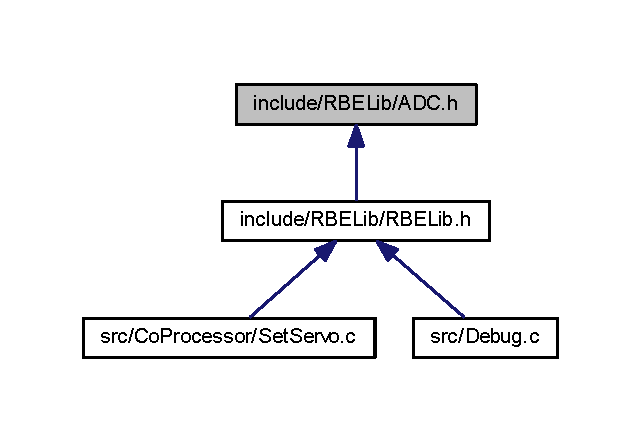
\includegraphics[width=308pt]{_a_d_c_8h__dep__incl}
\end{center}
\end{figure}
\subsection*{Functions}
\begin{DoxyCompactItemize}
\item 
void \hyperlink{_a_d_c_8h_a1f27a9e1c089f93efc89cdce78739cba}{init\-A\-D\-C} (int channel)
\begin{DoxyCompactList}\small\item\em Initializes the A\-D\-C and make one channel active. You can choose to use either interrupts or polling to read the desired channel. \end{DoxyCompactList}\item 
void \hyperlink{_a_d_c_8h_a3eef680fc13f11498db80fb145cab8f9}{clear\-A\-D\-C} (int channel)
\begin{DoxyCompactList}\small\item\em Disables A\-D\-C functionality and clears any saved values (globals). \end{DoxyCompactList}\item 
unsigned short \hyperlink{_a_d_c_8h_a9f560657fb624f98de3161651f3d4385}{get\-A\-D\-C} (int channel)
\begin{DoxyCompactList}\small\item\em Run a conversion on and get the analog value from one A\-D\-C channel if using polling. \end{DoxyCompactList}\item 
void \hyperlink{_a_d_c_8h_a8174ca24b578eaf4f82f44d6ce44edb0}{change\-A\-D\-C} (int channel)
\begin{DoxyCompactList}\small\item\em Change the channel the A\-D\-C is sampling if using interrupts. \end{DoxyCompactList}\end{DoxyCompactItemize}


\subsection{Detailed Description}
The header file and function prototypes for the A\-D\-C. For single ended conversion, the A\-D\-C value an be found from the voltage using\-: \[ \frac {V_{in} * 1024}{V_{ref}} \] \begin{DoxyAuthor}{Author}
Kevin Harrington 
\end{DoxyAuthor}
\begin{DoxyDate}{Date}
February 11, 2010
\end{DoxyDate}
\begin{DoxyAuthor}{Author}
Justin Barrett 
\end{DoxyAuthor}
\begin{DoxyDate}{Date}
August 23, 2011
\end{DoxyDate}
\begin{DoxyAuthor}{Author}
Eric Willcox 
\end{DoxyAuthor}
\begin{DoxyDate}{Date}
August 19, 2013 
\end{DoxyDate}


Definition in file \hyperlink{_a_d_c_8h_source}{A\-D\-C.\-h}.



\subsection{Function Documentation}
\hypertarget{_a_d_c_8h_a8174ca24b578eaf4f82f44d6ce44edb0}{\index{A\-D\-C.\-h@{A\-D\-C.\-h}!change\-A\-D\-C@{change\-A\-D\-C}}
\index{change\-A\-D\-C@{change\-A\-D\-C}!ADC.h@{A\-D\-C.\-h}}
\subsubsection[{change\-A\-D\-C}]{\setlength{\rightskip}{0pt plus 5cm}void change\-A\-D\-C (
\begin{DoxyParamCaption}
\item[{int}]{channel}
\end{DoxyParamCaption}
)}}\label{_a_d_c_8h_a8174ca24b578eaf4f82f44d6ce44edb0}


Change the channel the A\-D\-C is sampling if using interrupts. 


\begin{DoxyParams}{Parameters}
{\em channel} & The A\-D\-C channel to switch to.\\
\hline
\end{DoxyParams}
\begin{DoxyRefDesc}{Todo}
\item[\hyperlink{todo__todo000004}{Todo}]Create a way to switch A\-D\-C channels if you are using interrupts. \end{DoxyRefDesc}
\hypertarget{_a_d_c_8h_a3eef680fc13f11498db80fb145cab8f9}{\index{A\-D\-C.\-h@{A\-D\-C.\-h}!clear\-A\-D\-C@{clear\-A\-D\-C}}
\index{clear\-A\-D\-C@{clear\-A\-D\-C}!ADC.h@{A\-D\-C.\-h}}
\subsubsection[{clear\-A\-D\-C}]{\setlength{\rightskip}{0pt plus 5cm}void clear\-A\-D\-C (
\begin{DoxyParamCaption}
\item[{int}]{channel}
\end{DoxyParamCaption}
)}}\label{_a_d_c_8h_a3eef680fc13f11498db80fb145cab8f9}


Disables A\-D\-C functionality and clears any saved values (globals). 


\begin{DoxyParams}{Parameters}
{\em channel} & The A\-D\-C channel to disable.\\
\hline
\end{DoxyParams}
\begin{DoxyRefDesc}{Todo}
\item[\hyperlink{todo__todo000002}{Todo}]Create the corresponding function to clear the last A\-D\-C calculation register and disconnect the input to the A\-D\-C if desired. \end{DoxyRefDesc}
\hypertarget{_a_d_c_8h_a9f560657fb624f98de3161651f3d4385}{\index{A\-D\-C.\-h@{A\-D\-C.\-h}!get\-A\-D\-C@{get\-A\-D\-C}}
\index{get\-A\-D\-C@{get\-A\-D\-C}!ADC.h@{A\-D\-C.\-h}}
\subsubsection[{get\-A\-D\-C}]{\setlength{\rightskip}{0pt plus 5cm}unsigned short get\-A\-D\-C (
\begin{DoxyParamCaption}
\item[{int}]{channel}
\end{DoxyParamCaption}
)}}\label{_a_d_c_8h_a9f560657fb624f98de3161651f3d4385}


Run a conversion on and get the analog value from one A\-D\-C channel if using polling. 


\begin{DoxyParams}{Parameters}
{\em channel} & The A\-D\-C channel to run a conversion on. \\
\hline
\end{DoxyParams}
\begin{DoxyReturn}{Returns}
adc\-Val The 8-\/10 bit value returned by the A\-D\-C conversion. The precision depends on your settings and how much accuracy you desire.
\end{DoxyReturn}
\begin{DoxyRefDesc}{Todo}
\item[\hyperlink{todo__todo000003}{Todo}]Create the corresponding function to obtain the value of the last calculation if you are using polling. \end{DoxyRefDesc}
\hypertarget{_a_d_c_8h_a1f27a9e1c089f93efc89cdce78739cba}{\index{A\-D\-C.\-h@{A\-D\-C.\-h}!init\-A\-D\-C@{init\-A\-D\-C}}
\index{init\-A\-D\-C@{init\-A\-D\-C}!ADC.h@{A\-D\-C.\-h}}
\subsubsection[{init\-A\-D\-C}]{\setlength{\rightskip}{0pt plus 5cm}void init\-A\-D\-C (
\begin{DoxyParamCaption}
\item[{int}]{channel}
\end{DoxyParamCaption}
)}}\label{_a_d_c_8h_a1f27a9e1c089f93efc89cdce78739cba}


Initializes the A\-D\-C and make one channel active. You can choose to use either interrupts or polling to read the desired channel. 


\begin{DoxyParams}{Parameters}
{\em channel} & The A\-D\-C channel to initialize.\\
\hline
\end{DoxyParams}
\begin{DoxyRefDesc}{Todo}
\item[\hyperlink{todo__todo000001}{Todo}]Create the corresponding function to initialize the A\-D\-C using the channel parameter. \end{DoxyRefDesc}

\hypertarget{_d_a_c_8h}{\section{include/\-R\-B\-E\-Lib/\-D\-A\-C.h File Reference}
\label{_d_a_c_8h}\index{include/\-R\-B\-E\-Lib/\-D\-A\-C.\-h@{include/\-R\-B\-E\-Lib/\-D\-A\-C.\-h}}
}


The header file and function prototypes for the D\-A\-C.  


This graph shows which files directly or indirectly include this file\-:\nopagebreak
\begin{figure}[H]
\begin{center}
\leavevmode
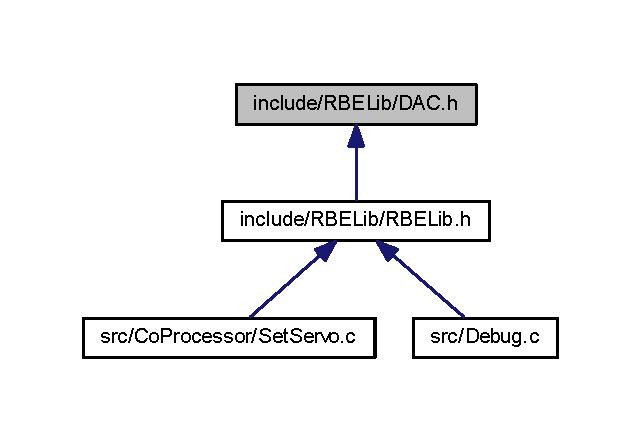
\includegraphics[width=308pt]{_d_a_c_8h__dep__incl}
\end{center}
\end{figure}
\subsection*{Functions}
\begin{DoxyCompactItemize}
\item 
void \hyperlink{_d_a_c_8h_af5aa1a81aa11a072a5ab582d040b3edf}{set\-D\-A\-C} (int D\-A\-Cn, int S\-P\-I\-Val)
\begin{DoxyCompactList}\small\item\em Set the D\-A\-C to the given value on the chosen channel. \end{DoxyCompactList}\end{DoxyCompactItemize}


\subsection{Detailed Description}
The header file and function prototypes for the D\-A\-C. Use these functions to control the behavior of the D\-A\-C. \begin{DoxyAuthor}{Author}
Eric Willcox 
\end{DoxyAuthor}
\begin{DoxyDate}{Date}
August 21, 2013 
\end{DoxyDate}


Definition in file \hyperlink{_d_a_c_8h_source}{D\-A\-C.\-h}.



\subsection{Function Documentation}
\hypertarget{_d_a_c_8h_af5aa1a81aa11a072a5ab582d040b3edf}{\index{D\-A\-C.\-h@{D\-A\-C.\-h}!set\-D\-A\-C@{set\-D\-A\-C}}
\index{set\-D\-A\-C@{set\-D\-A\-C}!DAC.h@{D\-A\-C.\-h}}
\subsubsection[{set\-D\-A\-C}]{\setlength{\rightskip}{0pt plus 5cm}void set\-D\-A\-C (
\begin{DoxyParamCaption}
\item[{int}]{D\-A\-Cn, }
\item[{int}]{S\-P\-I\-Val}
\end{DoxyParamCaption}
)}}\label{_d_a_c_8h_af5aa1a81aa11a072a5ab582d040b3edf}


Set the D\-A\-C to the given value on the chosen channel. 


\begin{DoxyParams}{Parameters}
{\em D\-A\-Cn} & The channel that you want to set. \\
\hline
{\em S\-P\-I\-Val} & The value you want to set it to.\\
\hline
\end{DoxyParams}
\begin{DoxyRefDesc}{Todo}
\item[\hyperlink{todo__todo000005}{Todo}]Make the function that is able to set the D\-A\-C to a given value from 0 -\/ 4095. \end{DoxyRefDesc}

\hypertarget{_debug_8h}{\section{include/\-R\-B\-E\-Lib/\-Debug.h File Reference}
\label{_debug_8h}\index{include/\-R\-B\-E\-Lib/\-Debug.\-h@{include/\-R\-B\-E\-Lib/\-Debug.\-h}}
}


Allows for the use of printf() on the 3001 board. Simply rebinds stdout to the U\-A\-R\-T.  


This graph shows which files directly or indirectly include this file\-:\nopagebreak
\begin{figure}[H]
\begin{center}
\leavevmode
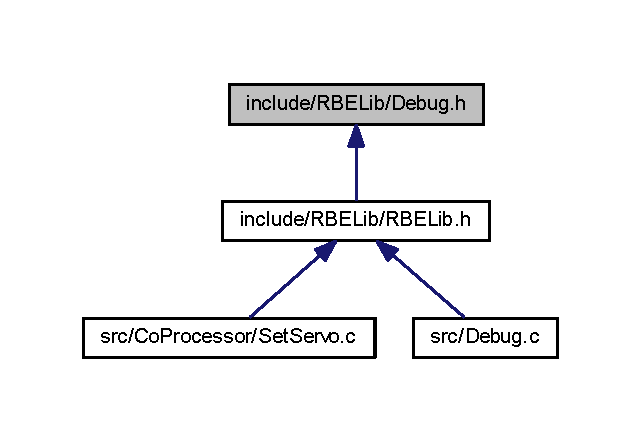
\includegraphics[width=308pt]{_debug_8h__dep__incl}
\end{center}
\end{figure}
\subsection*{Functions}
\begin{DoxyCompactItemize}
\item 
int \hyperlink{_debug_8h_a450add2014d3b1c410c4225da137269a}{printf\-R\-B\-E} (char var, F\-I\-L\-E $\ast$stream)
\begin{DoxyCompactList}\small\item\em Calls the students function '\hyperlink{_u_s_a_r_t_debug_8h_ab52220b9802762326175f5a6d09c50a1}{put\-Char\-Debug()}' to output the stream to. You should not call this function directly, instead use the standard function printf(). \end{DoxyCompactList}\item 
void \hyperlink{_debug_8h_af447ccfe0edd5c2eee6ff9aba36bd6f9}{init\-R\-B\-E\-Lib} ()
\begin{DoxyCompactList}\small\item\em Rebinds stdout to call \hyperlink{_debug_8h_a450add2014d3b1c410c4225da137269a}{printf\-R\-B\-E()} and initializes communication with the coprocessor. This function should be called once at the start of your code once you have \hyperlink{_u_s_a_r_t_debug_8h_ab52220b9802762326175f5a6d09c50a1}{put\-Char\-Debug()} written in Lab 1. If you do not call this, printf() and Set\-Servo() will not work. \end{DoxyCompactList}\end{DoxyCompactItemize}


\subsection{Detailed Description}
Allows for the use of printf() on the 3001 board. Simply rebinds stdout to the U\-A\-R\-T. \begin{DoxyAuthor}{Author}
Eric Willcox 
\end{DoxyAuthor}
\begin{DoxyDate}{Date}
July 9, 2014 
\end{DoxyDate}


Definition in file \hyperlink{_debug_8h_source}{Debug.\-h}.



\subsection{Function Documentation}
\hypertarget{_debug_8h_af447ccfe0edd5c2eee6ff9aba36bd6f9}{\index{Debug.\-h@{Debug.\-h}!init\-R\-B\-E\-Lib@{init\-R\-B\-E\-Lib}}
\index{init\-R\-B\-E\-Lib@{init\-R\-B\-E\-Lib}!Debug.h@{Debug.\-h}}
\subsubsection[{init\-R\-B\-E\-Lib}]{\setlength{\rightskip}{0pt plus 5cm}void init\-R\-B\-E\-Lib (
\begin{DoxyParamCaption}
{}
\end{DoxyParamCaption}
)}}\label{_debug_8h_af447ccfe0edd5c2eee6ff9aba36bd6f9}


Rebinds stdout to call \hyperlink{_debug_8h_a450add2014d3b1c410c4225da137269a}{printf\-R\-B\-E()} and initializes communication with the coprocessor. This function should be called once at the start of your code once you have \hyperlink{_u_s_a_r_t_debug_8h_ab52220b9802762326175f5a6d09c50a1}{put\-Char\-Debug()} written in Lab 1. If you do not call this, printf() and Set\-Servo() will not work. 



Definition at line 20 of file Debug.\-c.



References init\-Alt\-Com().



Here is the call graph for this function\-:\nopagebreak
\begin{figure}[H]
\begin{center}
\leavevmode
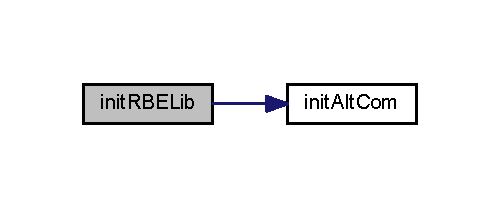
\includegraphics[width=240pt]{_debug_8h_af447ccfe0edd5c2eee6ff9aba36bd6f9_cgraph}
\end{center}
\end{figure}


\hypertarget{_debug_8h_a450add2014d3b1c410c4225da137269a}{\index{Debug.\-h@{Debug.\-h}!printf\-R\-B\-E@{printf\-R\-B\-E}}
\index{printf\-R\-B\-E@{printf\-R\-B\-E}!Debug.h@{Debug.\-h}}
\subsubsection[{printf\-R\-B\-E}]{\setlength{\rightskip}{0pt plus 5cm}int printf\-R\-B\-E (
\begin{DoxyParamCaption}
\item[{char}]{var, }
\item[{F\-I\-L\-E $\ast$}]{stream}
\end{DoxyParamCaption}
)}}\label{_debug_8h_a450add2014d3b1c410c4225da137269a}


Calls the students function '\hyperlink{_u_s_a_r_t_debug_8h_ab52220b9802762326175f5a6d09c50a1}{put\-Char\-Debug()}' to output the stream to. You should not call this function directly, instead use the standard function printf(). 


\begin{DoxyParams}{Parameters}
{\em var} & Character to output \\
\hline
{\em $\ast$stream} & Place to put the character (stdout) \\
\hline
\end{DoxyParams}


Definition at line 14 of file Debug.\-c.



References put\-Char\-Debug().



Here is the call graph for this function\-:\nopagebreak
\begin{figure}[H]
\begin{center}
\leavevmode
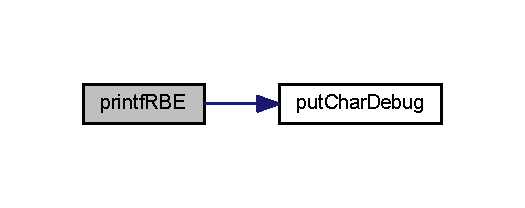
\includegraphics[width=252pt]{_debug_8h_a450add2014d3b1c410c4225da137269a_cgraph}
\end{center}
\end{figure}



\hypertarget{datatypes_8h}{\section{include/\-R\-B\-E\-Lib/doxy\-\_\-pages/datatypes.h File Reference}
\label{datatypes_8h}\index{include/\-R\-B\-E\-Lib/doxy\-\_\-pages/datatypes.\-h@{include/\-R\-B\-E\-Lib/doxy\-\_\-pages/datatypes.\-h}}
}


\subsection{Detailed Description}
Tells some of the common length of datatypes for your use. You can get this same data by doing
\begin{DoxyCode}
sizeOf(<datatype>); 
\end{DoxyCode}
 and printing out the value.

\begin{DoxyDate}{Date}
Aug 28, 2013 
\end{DoxyDate}
\begin{DoxyAuthor}{Author}
Eric Willcox 
\end{DoxyAuthor}


Definition in file \hyperlink{datatypes_8h_source}{datatypes.\-h}.


\hypertarget{index_8h}{\section{include/\-R\-B\-E\-Lib/doxy\-\_\-pages/index.h File Reference}
\label{index_8h}\index{include/\-R\-B\-E\-Lib/doxy\-\_\-pages/index.\-h@{include/\-R\-B\-E\-Lib/doxy\-\_\-pages/index.\-h}}
}


This is the index file for Doxygen that is used to link to everything.  




\subsection{Detailed Description}
This is the index file for Doxygen that is used to link to everything. \begin{DoxyAuthor}{Author}
Kevin Harrington 
\end{DoxyAuthor}
\begin{DoxyDate}{Date}
February 21, 2010 
\end{DoxyDate}
\begin{DoxyAuthor}{Author}
Eric Willcox 
\end{DoxyAuthor}
\begin{DoxyDate}{Date}
July 21, 2014 
\end{DoxyDate}


Definition in file \hyperlink{index_8h_source}{index.\-h}.


\hypertarget{motors_8h}{\section{include/\-R\-B\-E\-Lib/motors.h File Reference}
\label{motors_8h}\index{include/\-R\-B\-E\-Lib/motors.\-h@{include/\-R\-B\-E\-Lib/motors.\-h}}
}


Motor driving functions for the arm.  


This graph shows which files directly or indirectly include this file\-:\nopagebreak
\begin{figure}[H]
\begin{center}
\leavevmode
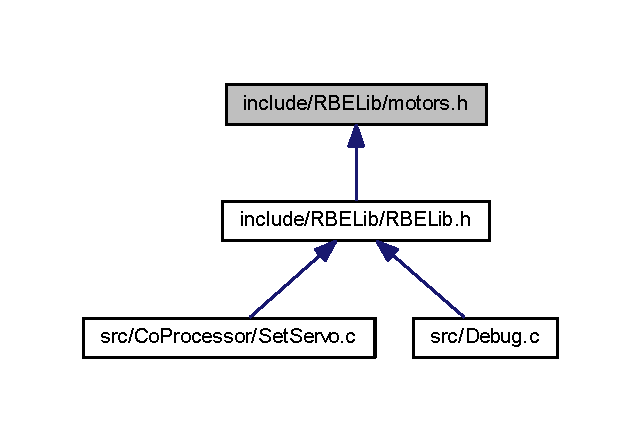
\includegraphics[width=308pt]{motors_8h__dep__incl}
\end{center}
\end{figure}
\subsection*{Functions}
\begin{DoxyCompactItemize}
\item 
void \hyperlink{motors_8h_a5260da8b51f5d97f6cf2a9ba11d1aee1}{stop\-Motors} ()
\begin{DoxyCompactList}\small\item\em Helper function to stop the motors on the arm. \end{DoxyCompactList}\item 
void \hyperlink{motors_8h_af29dc743a43c233ac843475727db132f}{goto\-Angles} (int lower\-Theta, int upper\-Theta)
\begin{DoxyCompactList}\small\item\em Drive the arm to a desired angle. \end{DoxyCompactList}\item 
void \hyperlink{motors_8h_aa294b49bfcc17cf4b490fb020e359851}{goto\-X\-Y} (int x, int y)
\begin{DoxyCompactList}\small\item\em Drive the end effector of the arm to a desired X and Y position in the workspace. \end{DoxyCompactList}\item 
void \hyperlink{motors_8h_af4a8cb121ce437984322ade3672082d2}{drive\-Link} (int link, int dir)
\begin{DoxyCompactList}\small\item\em Drive a link (upper or lower) in a desired direction. \end{DoxyCompactList}\item 
void \hyperlink{motors_8h_a946fb06843f118c8abacd3aef032584c}{home\-Pos} ()
\begin{DoxyCompactList}\small\item\em Drive the arm to a \char`\"{}home\char`\"{} position using the potentiometers. This should be called before using the encoders and just goes to a default position. Once this has been called once, you can initialize/clear the encoders. \end{DoxyCompactList}\end{DoxyCompactItemize}


\subsection{Detailed Description}
Motor driving functions for the arm. \begin{DoxyAuthor}{Author}
Eric Willcox 
\end{DoxyAuthor}
\begin{DoxyDate}{Date}
July 9, 2014 
\end{DoxyDate}


Definition in file \hyperlink{motors_8h_source}{motors.\-h}.



\subsection{Function Documentation}
\hypertarget{motors_8h_af4a8cb121ce437984322ade3672082d2}{\index{motors.\-h@{motors.\-h}!drive\-Link@{drive\-Link}}
\index{drive\-Link@{drive\-Link}!motors.h@{motors.\-h}}
\subsubsection[{drive\-Link}]{\setlength{\rightskip}{0pt plus 5cm}void drive\-Link (
\begin{DoxyParamCaption}
\item[{int}]{link, }
\item[{int}]{dir}
\end{DoxyParamCaption}
)}}\label{motors_8h_af4a8cb121ce437984322ade3672082d2}


Drive a link (upper or lower) in a desired direction. 


\begin{DoxyParams}{Parameters}
{\em link} & Which link to control. \\
\hline
{\em dir} & Which way to drive the link.\\
\hline
\end{DoxyParams}
\begin{DoxyRefDesc}{Todo}
\item[\hyperlink{todo__todo000009}{Todo}]Create a way to drive either link in any direction. \end{DoxyRefDesc}
\hypertarget{motors_8h_af29dc743a43c233ac843475727db132f}{\index{motors.\-h@{motors.\-h}!goto\-Angles@{goto\-Angles}}
\index{goto\-Angles@{goto\-Angles}!motors.h@{motors.\-h}}
\subsubsection[{goto\-Angles}]{\setlength{\rightskip}{0pt plus 5cm}void goto\-Angles (
\begin{DoxyParamCaption}
\item[{int}]{lower\-Theta, }
\item[{int}]{upper\-Theta}
\end{DoxyParamCaption}
)}}\label{motors_8h_af29dc743a43c233ac843475727db132f}


Drive the arm to a desired angle. 


\begin{DoxyParams}{Parameters}
{\em lower\-Theta} & The desired angle for the lower link. \\
\hline
{\em upper\-Theta} & The desired angle for the upper link.\\
\hline
\end{DoxyParams}
\begin{DoxyRefDesc}{Todo}
\item[\hyperlink{todo__todo000007}{Todo}]Make a way to drive the links to a desired angle. \end{DoxyRefDesc}
\hypertarget{motors_8h_aa294b49bfcc17cf4b490fb020e359851}{\index{motors.\-h@{motors.\-h}!goto\-X\-Y@{goto\-X\-Y}}
\index{goto\-X\-Y@{goto\-X\-Y}!motors.h@{motors.\-h}}
\subsubsection[{goto\-X\-Y}]{\setlength{\rightskip}{0pt plus 5cm}void goto\-X\-Y (
\begin{DoxyParamCaption}
\item[{int}]{x, }
\item[{int}]{y}
\end{DoxyParamCaption}
)}}\label{motors_8h_aa294b49bfcc17cf4b490fb020e359851}


Drive the end effector of the arm to a desired X and Y position in the workspace. 


\begin{DoxyParams}{Parameters}
{\em x} & The desired x position for the end effector. \\
\hline
{\em y} & The desired y position for the end effector.\\
\hline
\end{DoxyParams}
\begin{DoxyRefDesc}{Todo}
\item[\hyperlink{todo__todo000008}{Todo}]Use kinematic equations to move the end effector to the desired position. \end{DoxyRefDesc}
\hypertarget{motors_8h_a946fb06843f118c8abacd3aef032584c}{\index{motors.\-h@{motors.\-h}!home\-Pos@{home\-Pos}}
\index{home\-Pos@{home\-Pos}!motors.h@{motors.\-h}}
\subsubsection[{home\-Pos}]{\setlength{\rightskip}{0pt plus 5cm}void home\-Pos (
\begin{DoxyParamCaption}
{}
\end{DoxyParamCaption}
)}}\label{motors_8h_a946fb06843f118c8abacd3aef032584c}


Drive the arm to a \char`\"{}home\char`\"{} position using the potentiometers. This should be called before using the encoders and just goes to a default position. Once this has been called once, you can initialize/clear the encoders. 

\begin{DoxyRefDesc}{Todo}
\item[\hyperlink{todo__todo000010}{Todo}]Drive the arm to a known position using the potentiometers. \end{DoxyRefDesc}
\hypertarget{motors_8h_a5260da8b51f5d97f6cf2a9ba11d1aee1}{\index{motors.\-h@{motors.\-h}!stop\-Motors@{stop\-Motors}}
\index{stop\-Motors@{stop\-Motors}!motors.h@{motors.\-h}}
\subsubsection[{stop\-Motors}]{\setlength{\rightskip}{0pt plus 5cm}void stop\-Motors (
\begin{DoxyParamCaption}
{}
\end{DoxyParamCaption}
)}}\label{motors_8h_a5260da8b51f5d97f6cf2a9ba11d1aee1}


Helper function to stop the motors on the arm. 

\begin{DoxyRefDesc}{Todo}
\item[\hyperlink{todo__todo000006}{Todo}]Create way to stop the motors using the D\-A\-C. \end{DoxyRefDesc}

\hypertarget{_periph_8h}{\section{include/\-R\-B\-E\-Lib/\-Periph.h File Reference}
\label{_periph_8h}\index{include/\-R\-B\-E\-Lib/\-Periph.\-h@{include/\-R\-B\-E\-Lib/\-Periph.\-h}}
}


The header file and function prototypes for the peripherals (I\-R, encoder and accelerometer).  


This graph shows which files directly or indirectly include this file\-:\nopagebreak
\begin{figure}[H]
\begin{center}
\leavevmode
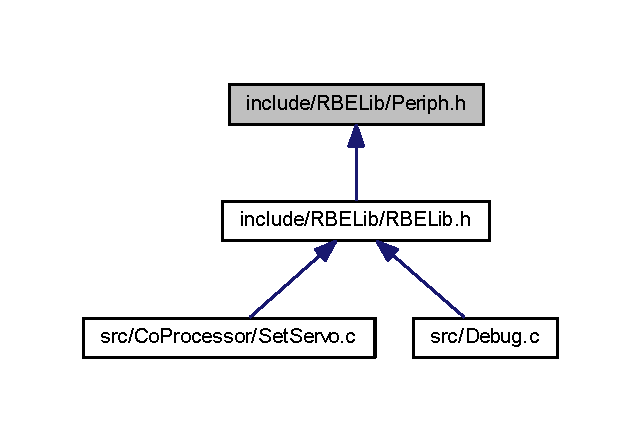
\includegraphics[width=308pt]{_periph_8h__dep__incl}
\end{center}
\end{figure}
\subsection*{Functions}
\begin{DoxyCompactItemize}
\item 
signed int \hyperlink{_periph_8h_a664961c139fdb66c6fd0fb0e997df433}{get\-Accel} (int axis)
\begin{DoxyCompactList}\small\item\em Find the acceleration in the given axis (X, Y, Z). \end{DoxyCompactList}\item 
int \hyperlink{_periph_8h_ae0fb6b592e76f0934db14682e63982df}{I\-R\-Dist} (int chan)
\begin{DoxyCompactList}\small\item\em Read an I\-R sensor and calculate the distance of the block. \end{DoxyCompactList}\item 
void \hyperlink{_periph_8h_a15de8c2dd97f966ce278ab793669adfd}{enc\-Init} (int chan)
\begin{DoxyCompactList}\small\item\em Initialize the encoders with the desired settings. \end{DoxyCompactList}\item 
void \hyperlink{_periph_8h_a9b159db17b7ebf680a2bdd169e269f85}{reset\-Enc\-Count} (int chan)
\begin{DoxyCompactList}\small\item\em Reset the current count of the encoder ticks. \end{DoxyCompactList}\item 
signed long \hyperlink{_periph_8h_a6c804bfcd9e9943d093395f535a3b672}{enc\-Count} (int chan)
\begin{DoxyCompactList}\small\item\em Finds the current count of one of the encoders. \end{DoxyCompactList}\end{DoxyCompactItemize}


\subsection{Detailed Description}
The header file and function prototypes for the peripherals (I\-R, encoder and accelerometer). Each of these functions is for controlling the peripheral devices of the arm. \begin{DoxyAuthor}{Author}
Eric Willcox 
\end{DoxyAuthor}
\begin{DoxyDate}{Date}
August 21, 2013 

July 18, 2014 
\end{DoxyDate}


Definition in file \hyperlink{_periph_8h_source}{Periph.\-h}.



\subsection{Function Documentation}
\hypertarget{_periph_8h_a6c804bfcd9e9943d093395f535a3b672}{\index{Periph.\-h@{Periph.\-h}!enc\-Count@{enc\-Count}}
\index{enc\-Count@{enc\-Count}!Periph.h@{Periph.\-h}}
\subsubsection[{enc\-Count}]{\setlength{\rightskip}{0pt plus 5cm}signed long enc\-Count (
\begin{DoxyParamCaption}
\item[{int}]{chan}
\end{DoxyParamCaption}
)}}\label{_periph_8h_a6c804bfcd9e9943d093395f535a3b672}


Finds the current count of one of the encoders. 


\begin{DoxyParams}{Parameters}
{\em chan} & Channel that the encoder is on that you would like to read. \\
\hline
\end{DoxyParams}
\begin{DoxyReturn}{Returns}
count The current count of the encoder.
\end{DoxyReturn}
\begin{DoxyRefDesc}{Todo}
\item[\hyperlink{todo__todo000015}{Todo}]Find the current encoder ticks on a given channel. \end{DoxyRefDesc}
\hypertarget{_periph_8h_a15de8c2dd97f966ce278ab793669adfd}{\index{Periph.\-h@{Periph.\-h}!enc\-Init@{enc\-Init}}
\index{enc\-Init@{enc\-Init}!Periph.h@{Periph.\-h}}
\subsubsection[{enc\-Init}]{\setlength{\rightskip}{0pt plus 5cm}void enc\-Init (
\begin{DoxyParamCaption}
\item[{int}]{chan}
\end{DoxyParamCaption}
)}}\label{_periph_8h_a15de8c2dd97f966ce278ab793669adfd}


Initialize the encoders with the desired settings. 


\begin{DoxyParams}{Parameters}
{\em chan} & Channel to initialize.\\
\hline
\end{DoxyParams}
\begin{DoxyRefDesc}{Todo}
\item[\hyperlink{todo__todo000013}{Todo}]Make a function that can setup both encoder chips on the board. \end{DoxyRefDesc}
\hypertarget{_periph_8h_a664961c139fdb66c6fd0fb0e997df433}{\index{Periph.\-h@{Periph.\-h}!get\-Accel@{get\-Accel}}
\index{get\-Accel@{get\-Accel}!Periph.h@{Periph.\-h}}
\subsubsection[{get\-Accel}]{\setlength{\rightskip}{0pt plus 5cm}signed int get\-Accel (
\begin{DoxyParamCaption}
\item[{int}]{axis}
\end{DoxyParamCaption}
)}}\label{_periph_8h_a664961c139fdb66c6fd0fb0e997df433}


Find the acceleration in the given axis (X, Y, Z). 


\begin{DoxyParams}{Parameters}
{\em axis} & The axis that you want to get the measurement of. \\
\hline
\end{DoxyParams}
\begin{DoxyReturn}{Returns}
g\-Val Value of acceleration.
\end{DoxyReturn}
\begin{DoxyRefDesc}{Todo}
\item[\hyperlink{todo__todo000011}{Todo}]Create a function that is able to find the acceleration of a given axis. \end{DoxyRefDesc}
\hypertarget{_periph_8h_ae0fb6b592e76f0934db14682e63982df}{\index{Periph.\-h@{Periph.\-h}!I\-R\-Dist@{I\-R\-Dist}}
\index{I\-R\-Dist@{I\-R\-Dist}!Periph.h@{Periph.\-h}}
\subsubsection[{I\-R\-Dist}]{\setlength{\rightskip}{0pt plus 5cm}int I\-R\-Dist (
\begin{DoxyParamCaption}
\item[{int}]{chan}
\end{DoxyParamCaption}
)}}\label{_periph_8h_ae0fb6b592e76f0934db14682e63982df}


Read an I\-R sensor and calculate the distance of the block. 


\begin{DoxyParams}{Parameters}
{\em chan} & The port that the I\-R sensor is on. \\
\hline
\end{DoxyParams}
\begin{DoxyReturn}{Returns}
value The distance the block is from the sensor.
\end{DoxyReturn}
\begin{DoxyRefDesc}{Todo}
\item[\hyperlink{todo__todo000012}{Todo}]Make a function that is able to get the A\-D\-C value of the I\-R sensor. \end{DoxyRefDesc}
\hypertarget{_periph_8h_a9b159db17b7ebf680a2bdd169e269f85}{\index{Periph.\-h@{Periph.\-h}!reset\-Enc\-Count@{reset\-Enc\-Count}}
\index{reset\-Enc\-Count@{reset\-Enc\-Count}!Periph.h@{Periph.\-h}}
\subsubsection[{reset\-Enc\-Count}]{\setlength{\rightskip}{0pt plus 5cm}void reset\-Enc\-Count (
\begin{DoxyParamCaption}
\item[{int}]{chan}
\end{DoxyParamCaption}
)}}\label{_periph_8h_a9b159db17b7ebf680a2bdd169e269f85}


Reset the current count of the encoder ticks. 


\begin{DoxyParams}{Parameters}
{\em chan} & The channel to clear.\\
\hline
\end{DoxyParams}
\begin{DoxyRefDesc}{Todo}
\item[\hyperlink{todo__todo000014}{Todo}]Clear the encoder count (set to 0). \end{DoxyRefDesc}

\hypertarget{_p_i_d_8h}{\section{include/\-R\-B\-E\-Lib/\-P\-I\-D.h File Reference}
\label{_p_i_d_8h}\index{include/\-R\-B\-E\-Lib/\-P\-I\-D.\-h@{include/\-R\-B\-E\-Lib/\-P\-I\-D.\-h}}
}


The header file for P\-I\-D constants and calculations.  


This graph shows which files directly or indirectly include this file\-:\nopagebreak
\begin{figure}[H]
\begin{center}
\leavevmode
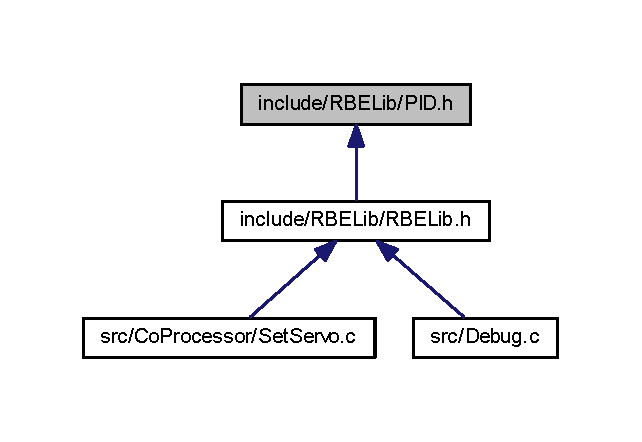
\includegraphics[width=308pt]{_p_i_d_8h__dep__incl}
\end{center}
\end{figure}
\subsection*{Data Structures}
\begin{DoxyCompactItemize}
\item 
struct \hyperlink{structpid_const}{pid\-Const}
\begin{DoxyCompactList}\small\item\em P\-I\-D constants. \end{DoxyCompactList}\end{DoxyCompactItemize}
\subsection*{Functions}
\begin{DoxyCompactItemize}
\item 
void \hyperlink{_p_i_d_8h_a2ffb511c1e18ce767f42422609dfa04d}{set\-Const} (char link, float Kp, float Ki, float Kd)
\begin{DoxyCompactList}\small\item\em Sets the Kp, Ki, and Kd values for 1 link. \end{DoxyCompactList}\item 
signed int \hyperlink{_p_i_d_8h_a0b728f39f71526d44fd7cff0ce67319e}{calc\-P\-I\-D} (char link, int set\-Point, int act\-Pos)
\begin{DoxyCompactList}\small\item\em Calculate the P\-I\-D value. \end{DoxyCompactList}\end{DoxyCompactItemize}
\subsection*{Variables}
\begin{DoxyCompactItemize}
\item 
\hyperlink{structpid_const}{pid\-Const} \hyperlink{_p_i_d_8h_a4d2fc78b5924045bcc0e20fc95e18d97}{pid\-Consts}
\begin{DoxyCompactList}\small\item\em Declaration for use in other files. \end{DoxyCompactList}\end{DoxyCompactItemize}


\subsection{Detailed Description}
The header file for P\-I\-D constants and calculations. Sets the P\-I\-D constants and calculate the P\-I\-D value. \begin{DoxyAuthor}{Author}
Eric Willcox 
\end{DoxyAuthor}
\begin{DoxyDate}{Date}
August 17 2013 
\end{DoxyDate}


Definition in file \hyperlink{_p_i_d_8h_source}{P\-I\-D.\-h}.



\subsection{Function Documentation}
\hypertarget{_p_i_d_8h_a0b728f39f71526d44fd7cff0ce67319e}{\index{P\-I\-D.\-h@{P\-I\-D.\-h}!calc\-P\-I\-D@{calc\-P\-I\-D}}
\index{calc\-P\-I\-D@{calc\-P\-I\-D}!PID.h@{P\-I\-D.\-h}}
\subsubsection[{calc\-P\-I\-D}]{\setlength{\rightskip}{0pt plus 5cm}signed int calc\-P\-I\-D (
\begin{DoxyParamCaption}
\item[{char}]{link, }
\item[{int}]{set\-Point, }
\item[{int}]{act\-Pos}
\end{DoxyParamCaption}
)}}\label{_p_i_d_8h_a0b728f39f71526d44fd7cff0ce67319e}


Calculate the P\-I\-D value. 


\begin{DoxyParams}{Parameters}
{\em link} & Which link to calculate the error for (Use 'U' and 'L'). \\
\hline
{\em set\-Point} & The desired position of the link. \\
\hline
{\em act\-Pos} & The current position of the link.\\
\hline
\end{DoxyParams}
\begin{DoxyRefDesc}{Todo}
\item[\hyperlink{todo__todo000018}{Todo}]Make a function to calculate the P\-I\-D value for a link. \end{DoxyRefDesc}
\hypertarget{_p_i_d_8h_a2ffb511c1e18ce767f42422609dfa04d}{\index{P\-I\-D.\-h@{P\-I\-D.\-h}!set\-Const@{set\-Const}}
\index{set\-Const@{set\-Const}!PID.h@{P\-I\-D.\-h}}
\subsubsection[{set\-Const}]{\setlength{\rightskip}{0pt plus 5cm}void set\-Const (
\begin{DoxyParamCaption}
\item[{char}]{link, }
\item[{float}]{Kp, }
\item[{float}]{Ki, }
\item[{float}]{Kd}
\end{DoxyParamCaption}
)}}\label{_p_i_d_8h_a2ffb511c1e18ce767f42422609dfa04d}


Sets the Kp, Ki, and Kd values for 1 link. 

to set the values, use the following style 
\begin{DoxyCode}
\hyperlink{structpid_const}{pidConst}.Kp = 1.3; 
\end{DoxyCode}
 
\begin{DoxyParams}{Parameters}
{\em link} & The link you want to set the values for (H or L). \\
\hline
{\em Kp} & Proportional value. \\
\hline
{\em Ki} & Integral value. \\
\hline
{\em Kd} & Derivative value.\\
\hline
\end{DoxyParams}
\begin{DoxyRefDesc}{Todo}
\item[\hyperlink{todo__todo000017}{Todo}]Create a function to the the P\-I\-D constants for a given link. \end{DoxyRefDesc}


\subsection{Variable Documentation}
\hypertarget{_p_i_d_8h_a4d2fc78b5924045bcc0e20fc95e18d97}{\index{P\-I\-D.\-h@{P\-I\-D.\-h}!pid\-Consts@{pid\-Consts}}
\index{pid\-Consts@{pid\-Consts}!PID.h@{P\-I\-D.\-h}}
\subsubsection[{pid\-Consts}]{\setlength{\rightskip}{0pt plus 5cm}{\bf pid\-Const} pid\-Consts}}\label{_p_i_d_8h_a4d2fc78b5924045bcc0e20fc95e18d97}


Declaration for use in other files. 

\begin{DoxyRefDesc}{Todo}
\item[\hyperlink{todo__todo000016}{Todo}]Again, do not forget to use\end{DoxyRefDesc}

\begin{DoxyCode}
\hyperlink{structpid_const}{pidConst} pidConsts; 
\end{DoxyCode}
 in any file you access them in! 
\hypertarget{ports_8h}{\section{include/\-R\-B\-E\-Lib/ports.h File Reference}
\label{ports_8h}\index{include/\-R\-B\-E\-Lib/ports.\-h@{include/\-R\-B\-E\-Lib/ports.\-h}}
}


Controls ports A -\/ D to be able to set direction, read a value and set a value for any pins desired.  


This graph shows which files directly or indirectly include this file\-:\nopagebreak
\begin{figure}[H]
\begin{center}
\leavevmode
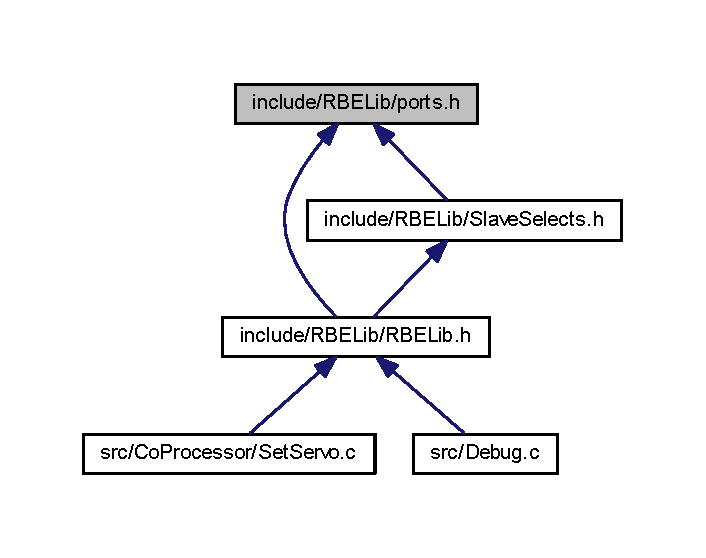
\includegraphics[width=339pt]{ports_8h__dep__incl}
\end{center}
\end{figure}
\subsection*{Functions}
\begin{DoxyCompactItemize}
\item 
void \hyperlink{ports_8h_a1b62a36451c75cf20221c12f039ad6f4}{set\-Pins\-Dir} (char port, int dir, char num\-Pins,...)
\begin{DoxyCompactList}\small\item\em Sets the direction (Input/\-Output) of the specified pins. \end{DoxyCompactList}\item 
unsigned char \hyperlink{ports_8h_a85e9d6d0f75513f3f961c41861299430}{get\-Pins\-Val} (char port, int num\-Pins,...)
\begin{DoxyCompactList}\small\item\em Gets the value on the specified pins of a port. \end{DoxyCompactList}\item 
void \hyperlink{ports_8h_afd809b04181b31d8567d95f070bb9034}{set\-Pins\-Val} (char port, int val, int num\-Pins,...)
\begin{DoxyCompactList}\small\item\em Sets the value on the specified pins of a port. \end{DoxyCompactList}\end{DoxyCompactItemize}


\subsection{Detailed Description}
Controls ports A -\/ D to be able to set direction, read a value and set a value for any pins desired. All functions here can take in a variable number of pins to set/read from. The way this is accomplished in C is by using the functions provided by stdarg.\-h and is the way that printf() works in the standard library.

While an array could be used just as well, a variable number of arguments is used to give exposure to variable arguments.

An example of how to call a function with variable arguments can look like this for calling \hyperlink{ports_8h_a1b62a36451c75cf20221c12f039ad6f4}{set\-Pins\-Dir()}.


\begin{DoxyCode}
\hyperlink{ports_8h_a1b62a36451c75cf20221c12f039ad6f4}{setPinsDir}(\textcolor{charliteral}{'A'}, \hyperlink{_r_b_e_lib_8h_a1bb283bd7893b9855e2f23013891fc82}{INPUT}, 2, 0, 5) 
\end{DoxyCode}


which sets 2 pins on Port A as inputs\-: 0 and 5.

An example has been created on the R\-B\-E wiki and can be found \href{http://wiki.wpi.edu/robotics/Programming_Background#Taking_in_a_Variable_Number_of_Arguments}{\tt here.}

\begin{DoxyAuthor}{Author}
Eric Willcox 
\end{DoxyAuthor}
\begin{DoxyDate}{Date}
July 18, 2014 
\end{DoxyDate}


Definition in file \hyperlink{ports_8h_source}{ports.\-h}.



\subsection{Function Documentation}
\hypertarget{ports_8h_a85e9d6d0f75513f3f961c41861299430}{\index{ports.\-h@{ports.\-h}!get\-Pins\-Val@{get\-Pins\-Val}}
\index{get\-Pins\-Val@{get\-Pins\-Val}!ports.h@{ports.\-h}}
\subsubsection[{get\-Pins\-Val}]{\setlength{\rightskip}{0pt plus 5cm}unsigned char get\-Pins\-Val (
\begin{DoxyParamCaption}
\item[{char}]{port, }
\item[{int}]{num\-Pins, }
\item[{}]{...}
\end{DoxyParamCaption}
)}}\label{ports_8h_a85e9d6d0f75513f3f961c41861299430}


Gets the value on the specified pins of a port. 


\begin{DoxyParams}{Parameters}
{\em port} & Port to read (A/\-B/\-C/\-D). \\
\hline
{\em num\-Pins} & The number of pins that you are reading. \\
\hline
{\em ...} & The pins one after another.\\
\hline
\end{DoxyParams}
\begin{DoxyReturn}{Returns}
value The value of the specified pins on the port.
\end{DoxyReturn}
\begin{DoxyRefDesc}{Todo}
\item[\hyperlink{todo__todo000020}{Todo}]Create a way to read all given pins on a port. \end{DoxyRefDesc}
\hypertarget{ports_8h_a1b62a36451c75cf20221c12f039ad6f4}{\index{ports.\-h@{ports.\-h}!set\-Pins\-Dir@{set\-Pins\-Dir}}
\index{set\-Pins\-Dir@{set\-Pins\-Dir}!ports.h@{ports.\-h}}
\subsubsection[{set\-Pins\-Dir}]{\setlength{\rightskip}{0pt plus 5cm}void set\-Pins\-Dir (
\begin{DoxyParamCaption}
\item[{char}]{port, }
\item[{int}]{dir, }
\item[{char}]{num\-Pins, }
\item[{}]{...}
\end{DoxyParamCaption}
)}}\label{ports_8h_a1b62a36451c75cf20221c12f039ad6f4}


Sets the direction (Input/\-Output) of the specified pins. 


\begin{DoxyParams}{Parameters}
{\em port} & Port to set (A/\-B/\-C/\-D). \\
\hline
{\em dir} & The pin on P\-O\-R\-T\-A to set the direction of. \\
\hline
{\em num\-Pins} & The number of pins that you are setting the direction of. \\
\hline
{\em ...} & Pins one after another\\
\hline
\end{DoxyParams}
\begin{DoxyRefDesc}{Todo}
\item[\hyperlink{todo__todo000019}{Todo}]Create a way to set a port's pins to inputs or outputs. \end{DoxyRefDesc}
\hypertarget{ports_8h_afd809b04181b31d8567d95f070bb9034}{\index{ports.\-h@{ports.\-h}!set\-Pins\-Val@{set\-Pins\-Val}}
\index{set\-Pins\-Val@{set\-Pins\-Val}!ports.h@{ports.\-h}}
\subsubsection[{set\-Pins\-Val}]{\setlength{\rightskip}{0pt plus 5cm}void set\-Pins\-Val (
\begin{DoxyParamCaption}
\item[{char}]{port, }
\item[{int}]{val, }
\item[{int}]{num\-Pins, }
\item[{}]{...}
\end{DoxyParamCaption}
)}}\label{ports_8h_afd809b04181b31d8567d95f070bb9034}


Sets the value on the specified pins of a port. 


\begin{DoxyParams}{Parameters}
{\em port} & Port to set (A/\-B/\-C/\-D). \\
\hline
{\em num\-Pins} & The number of pins that you are setting. \\
\hline
{\em val} & The value (high/low) to set the pin to. \\
\hline
{\em ...} & The pins one after another.\\
\hline
\end{DoxyParams}
\begin{DoxyRefDesc}{Todo}
\item[\hyperlink{todo__todo000021}{Todo}]Create a way to set all given pins on a port. \end{DoxyRefDesc}

\hypertarget{pot_8h}{\section{include/\-R\-B\-E\-Lib/pot.h File Reference}
\label{pot_8h}\index{include/\-R\-B\-E\-Lib/pot.\-h@{include/\-R\-B\-E\-Lib/pot.\-h}}
}


The header file and function prototypes for the potentiometers.  


This graph shows which files directly or indirectly include this file\-:\nopagebreak
\begin{figure}[H]
\begin{center}
\leavevmode
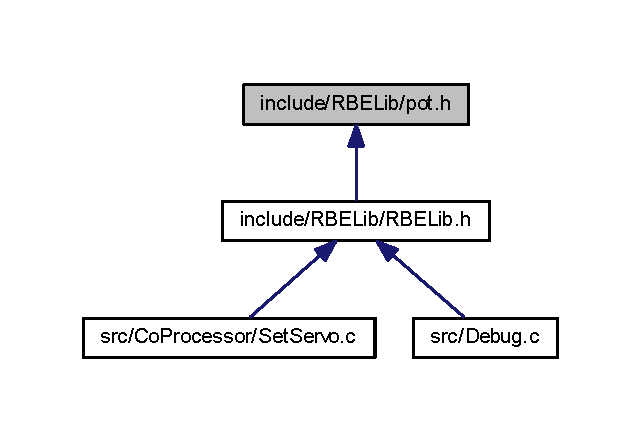
\includegraphics[width=308pt]{pot_8h__dep__incl}
\end{center}
\end{figure}
\subsection*{Functions}
\begin{DoxyCompactItemize}
\item 
int \hyperlink{pot_8h_a6572afa21880ee8fe8e834b7167e111b}{pot\-Angle} (int pot)
\begin{DoxyCompactList}\small\item\em Find the angle of the given potentiometer. \end{DoxyCompactList}\item 
int \hyperlink{pot_8h_ac8f71572a099805fc4cfcc793260e98b}{pot\-Volts} (int pot)
\begin{DoxyCompactList}\small\item\em Find the voltage value of the given potentiometer. \end{DoxyCompactList}\end{DoxyCompactItemize}


\subsection{Detailed Description}
The header file and function prototypes for the potentiometers. Use these functions to read the values from the pots. \begin{DoxyAuthor}{Author}
Eric Willcox 
\end{DoxyAuthor}
\begin{DoxyDate}{Date}
August 17 2013 
\end{DoxyDate}


Definition in file \hyperlink{pot_8h_source}{pot.\-h}.



\subsection{Function Documentation}
\hypertarget{pot_8h_a6572afa21880ee8fe8e834b7167e111b}{\index{pot.\-h@{pot.\-h}!pot\-Angle@{pot\-Angle}}
\index{pot\-Angle@{pot\-Angle}!pot.h@{pot.\-h}}
\subsubsection[{pot\-Angle}]{\setlength{\rightskip}{0pt plus 5cm}int pot\-Angle (
\begin{DoxyParamCaption}
\item[{int}]{pot}
\end{DoxyParamCaption}
)}}\label{pot_8h_a6572afa21880ee8fe8e834b7167e111b}


Find the angle of the given potentiometer. 


\begin{DoxyParams}{Parameters}
{\em pot} & The pot to check. \\
\hline
\end{DoxyParams}
\begin{DoxyReturn}{Returns}
angle Angle of the potentiometer.
\end{DoxyReturn}
\begin{DoxyRefDesc}{Todo}
\item[\hyperlink{todo__todo000022}{Todo}]Calculate the angle using the A\-D\-C reading. \end{DoxyRefDesc}
\hypertarget{pot_8h_ac8f71572a099805fc4cfcc793260e98b}{\index{pot.\-h@{pot.\-h}!pot\-Volts@{pot\-Volts}}
\index{pot\-Volts@{pot\-Volts}!pot.h@{pot.\-h}}
\subsubsection[{pot\-Volts}]{\setlength{\rightskip}{0pt plus 5cm}int pot\-Volts (
\begin{DoxyParamCaption}
\item[{int}]{pot}
\end{DoxyParamCaption}
)}}\label{pot_8h_ac8f71572a099805fc4cfcc793260e98b}


Find the voltage value of the given potentiometer. 


\begin{DoxyParams}{Parameters}
{\em pot} & The pot to get the value of. \\
\hline
\end{DoxyParams}
\begin{DoxyReturn}{Returns}
volts Voltage of potentiometer.
\end{DoxyReturn}
\begin{DoxyRefDesc}{Todo}
\item[\hyperlink{todo__todo000023}{Todo}]Convert the A\-D\-C value into a voltage in m\-V (so no floats needed). \end{DoxyRefDesc}

\hypertarget{_r_b_e_lib_8h}{\section{include/\-R\-B\-E\-Lib/\-R\-B\-E\-Lib.h File Reference}
\label{_r_b_e_lib_8h}\index{include/\-R\-B\-E\-Lib/\-R\-B\-E\-Lib.\-h@{include/\-R\-B\-E\-Lib/\-R\-B\-E\-Lib.\-h}}
}


This is a meta-\/header. It includes all the other header files that are needed for R\-B\-E\-Lib as well as some macros.  


{\ttfamily \#include $<$util/delay.\-h$>$}\\*
{\ttfamily \#include $<$avr/io.\-h$>$}\\*
{\ttfamily \#include $<$avr/interrupt.\-h$>$}\\*
{\ttfamily \#include $<$string.\-h$>$}\\*
{\ttfamily \#include $<$stdarg.\-h$>$}\\*
{\ttfamily \#include $<$stdio.\-h$>$}\\*
{\ttfamily \#include \char`\"{}A\-D\-C.\-h\char`\"{}}\\*
{\ttfamily \#include \char`\"{}D\-A\-C.\-h\char`\"{}}\\*
{\ttfamily \#include \char`\"{}Debug.\-h\char`\"{}}\\*
{\ttfamily \#include \char`\"{}motors.\-h\char`\"{}}\\*
{\ttfamily \#include \char`\"{}U\-S\-A\-R\-T\-Debug.\-h\char`\"{}}\\*
{\ttfamily \#include \char`\"{}timer.\-h\char`\"{}}\\*
{\ttfamily \#include \char`\"{}Periph.\-h\char`\"{}}\\*
{\ttfamily \#include \char`\"{}pot.\-h\char`\"{}}\\*
{\ttfamily \#include \char`\"{}P\-I\-D.\-h\char`\"{}}\\*
{\ttfamily \#include \char`\"{}reg\-\_\-structs.\-h\char`\"{}}\\*
{\ttfamily \#include \char`\"{}ports.\-h\char`\"{}}\\*
{\ttfamily \#include \char`\"{}S\-P\-I.\-h\char`\"{}}\\*
{\ttfamily \#include \char`\"{}Set\-Servo.\-h\char`\"{}}\\*
{\ttfamily \#include \char`\"{}Slave\-Selects.\-h\char`\"{}}\\*
Include dependency graph for R\-B\-E\-Lib.\-h\-:\nopagebreak
\begin{figure}[H]
\begin{center}
\leavevmode
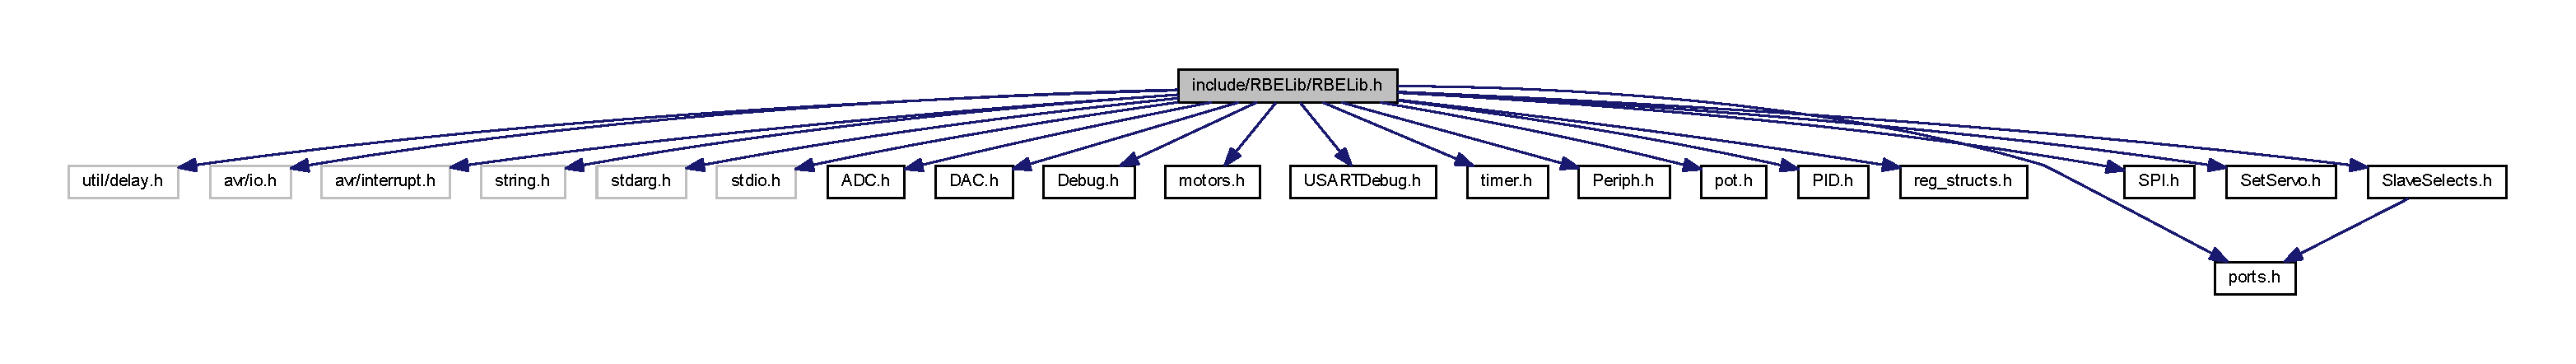
\includegraphics[width=350pt]{_r_b_e_lib_8h__incl}
\end{center}
\end{figure}
This graph shows which files directly or indirectly include this file\-:\nopagebreak
\begin{figure}[H]
\begin{center}
\leavevmode
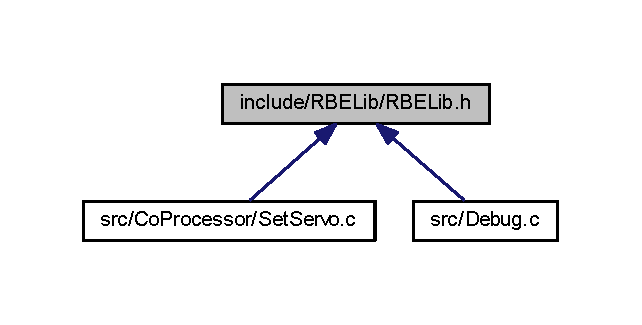
\includegraphics[width=308pt]{_r_b_e_lib_8h__dep__incl}
\end{center}
\end{figure}
\subsection*{Macros}
\begin{DoxyCompactItemize}
\item 
\#define \hyperlink{_r_b_e_lib_8h_a61a3c9a18380aafb6e430e79bf596557}{O\-U\-T\-P\-U\-T}~1
\item 
\#define \hyperlink{_r_b_e_lib_8h_a1bb283bd7893b9855e2f23013891fc82}{I\-N\-P\-U\-T}~0
\item 
\#define \hyperlink{_r_b_e_lib_8h_ad76d1750a6cdeebd506bfcd6752554d2}{O\-N}~1
\item 
\#define \hyperlink{_r_b_e_lib_8h_a29e413f6725b2ba32d165ffaa35b01e5}{O\-F\-F}~0
\item 
\#define \hyperlink{_r_b_e_lib_8h_a5bb885982ff66a2e0a0a45a8ee9c35e2}{H\-I\-G\-H}~1
\item 
\#define \hyperlink{_r_b_e_lib_8h_ab811d8c6ff3a505312d3276590444289}{L\-O\-W}~0
\item 
\#define \hyperlink{_r_b_e_lib_8h_aa8cecfc5c5c054d2875c03e77b7be15d}{T\-R\-U\-E}~1
\item 
\#define \hyperlink{_r_b_e_lib_8h_aa93f0eb578d23995850d61f7d61c55c1}{F\-A\-L\-S\-E}~0
\item 
\#define \hyperlink{_r_b_e_lib_8h_ae4cc35dcc70810fa972cc8a5185a28fa}{B\-O\-O\-L}~unsigned char
\item 
\#define \hyperlink{_r_b_e_lib_8h_aec93e83855ac17c3c25c55c37ca186dd}{B\-Y\-T\-E}~unsigned char
\item 
\#define \hyperlink{_r_b_e_lib_8h_a69afa2e50b905f4eab1f2df8a3fd9f23}{U\-I\-N\-T32}~unsigned long
\item 
\#define \hyperlink{_r_b_e_lib_8h_aac92c5ec332dafe0abb24688dad1b795}{I\-N\-T32}~long
\item 
\#define \hyperlink{_r_b_e_lib_8h_ab1922c2d8643eb7da964d427604e992e}{U\-I\-N\-T16}~unsigned short int
\item 
\#define \hyperlink{_r_b_e_lib_8h_a4cfc63e05db4883dc4b60a1245a9ffc5}{W\-O\-R\-D}~unsigned short int
\end{DoxyCompactItemize}


\subsection{Detailed Description}
This is a meta-\/header. It includes all the other header files that are needed for R\-B\-E\-Lib as well as some macros. \begin{DoxyAuthor}{Author}
Kevin Harrington 
\end{DoxyAuthor}
\begin{DoxyDate}{Date}
February 21, 2010
\end{DoxyDate}
\begin{DoxyAuthor}{Author}
Justin Barrett 
\end{DoxyAuthor}
\begin{DoxyDate}{Date}
August 23, 2011
\end{DoxyDate}
\begin{DoxyAuthor}{Author}
Eric Willcox 
\end{DoxyAuthor}
\begin{DoxyDate}{Date}
August 19, 2013 
\end{DoxyDate}


Definition in file \hyperlink{_r_b_e_lib_8h_source}{R\-B\-E\-Lib.\-h}.



\subsection{Macro Definition Documentation}
\hypertarget{_r_b_e_lib_8h_ae4cc35dcc70810fa972cc8a5185a28fa}{\index{R\-B\-E\-Lib.\-h@{R\-B\-E\-Lib.\-h}!B\-O\-O\-L@{B\-O\-O\-L}}
\index{B\-O\-O\-L@{B\-O\-O\-L}!RBELib.h@{R\-B\-E\-Lib.\-h}}
\subsubsection[{B\-O\-O\-L}]{\setlength{\rightskip}{0pt plus 5cm}\#define B\-O\-O\-L~unsigned char}}\label{_r_b_e_lib_8h_ae4cc35dcc70810fa972cc8a5185a28fa}


Definition at line 39 of file R\-B\-E\-Lib.\-h.

\hypertarget{_r_b_e_lib_8h_aec93e83855ac17c3c25c55c37ca186dd}{\index{R\-B\-E\-Lib.\-h@{R\-B\-E\-Lib.\-h}!B\-Y\-T\-E@{B\-Y\-T\-E}}
\index{B\-Y\-T\-E@{B\-Y\-T\-E}!RBELib.h@{R\-B\-E\-Lib.\-h}}
\subsubsection[{B\-Y\-T\-E}]{\setlength{\rightskip}{0pt plus 5cm}\#define B\-Y\-T\-E~unsigned char}}\label{_r_b_e_lib_8h_aec93e83855ac17c3c25c55c37ca186dd}


Definition at line 40 of file R\-B\-E\-Lib.\-h.

\hypertarget{_r_b_e_lib_8h_aa93f0eb578d23995850d61f7d61c55c1}{\index{R\-B\-E\-Lib.\-h@{R\-B\-E\-Lib.\-h}!F\-A\-L\-S\-E@{F\-A\-L\-S\-E}}
\index{F\-A\-L\-S\-E@{F\-A\-L\-S\-E}!RBELib.h@{R\-B\-E\-Lib.\-h}}
\subsubsection[{F\-A\-L\-S\-E}]{\setlength{\rightskip}{0pt plus 5cm}\#define F\-A\-L\-S\-E~0}}\label{_r_b_e_lib_8h_aa93f0eb578d23995850d61f7d61c55c1}


Definition at line 36 of file R\-B\-E\-Lib.\-h.

\hypertarget{_r_b_e_lib_8h_a5bb885982ff66a2e0a0a45a8ee9c35e2}{\index{R\-B\-E\-Lib.\-h@{R\-B\-E\-Lib.\-h}!H\-I\-G\-H@{H\-I\-G\-H}}
\index{H\-I\-G\-H@{H\-I\-G\-H}!RBELib.h@{R\-B\-E\-Lib.\-h}}
\subsubsection[{H\-I\-G\-H}]{\setlength{\rightskip}{0pt plus 5cm}\#define H\-I\-G\-H~1}}\label{_r_b_e_lib_8h_a5bb885982ff66a2e0a0a45a8ee9c35e2}


Definition at line 33 of file R\-B\-E\-Lib.\-h.

\hypertarget{_r_b_e_lib_8h_a1bb283bd7893b9855e2f23013891fc82}{\index{R\-B\-E\-Lib.\-h@{R\-B\-E\-Lib.\-h}!I\-N\-P\-U\-T@{I\-N\-P\-U\-T}}
\index{I\-N\-P\-U\-T@{I\-N\-P\-U\-T}!RBELib.h@{R\-B\-E\-Lib.\-h}}
\subsubsection[{I\-N\-P\-U\-T}]{\setlength{\rightskip}{0pt plus 5cm}\#define I\-N\-P\-U\-T~0}}\label{_r_b_e_lib_8h_a1bb283bd7893b9855e2f23013891fc82}


Definition at line 30 of file R\-B\-E\-Lib.\-h.

\hypertarget{_r_b_e_lib_8h_aac92c5ec332dafe0abb24688dad1b795}{\index{R\-B\-E\-Lib.\-h@{R\-B\-E\-Lib.\-h}!I\-N\-T32@{I\-N\-T32}}
\index{I\-N\-T32@{I\-N\-T32}!RBELib.h@{R\-B\-E\-Lib.\-h}}
\subsubsection[{I\-N\-T32}]{\setlength{\rightskip}{0pt plus 5cm}\#define I\-N\-T32~long}}\label{_r_b_e_lib_8h_aac92c5ec332dafe0abb24688dad1b795}


Definition at line 42 of file R\-B\-E\-Lib.\-h.

\hypertarget{_r_b_e_lib_8h_ab811d8c6ff3a505312d3276590444289}{\index{R\-B\-E\-Lib.\-h@{R\-B\-E\-Lib.\-h}!L\-O\-W@{L\-O\-W}}
\index{L\-O\-W@{L\-O\-W}!RBELib.h@{R\-B\-E\-Lib.\-h}}
\subsubsection[{L\-O\-W}]{\setlength{\rightskip}{0pt plus 5cm}\#define L\-O\-W~0}}\label{_r_b_e_lib_8h_ab811d8c6ff3a505312d3276590444289}


Definition at line 34 of file R\-B\-E\-Lib.\-h.

\hypertarget{_r_b_e_lib_8h_a29e413f6725b2ba32d165ffaa35b01e5}{\index{R\-B\-E\-Lib.\-h@{R\-B\-E\-Lib.\-h}!O\-F\-F@{O\-F\-F}}
\index{O\-F\-F@{O\-F\-F}!RBELib.h@{R\-B\-E\-Lib.\-h}}
\subsubsection[{O\-F\-F}]{\setlength{\rightskip}{0pt plus 5cm}\#define O\-F\-F~0}}\label{_r_b_e_lib_8h_a29e413f6725b2ba32d165ffaa35b01e5}


Definition at line 32 of file R\-B\-E\-Lib.\-h.

\hypertarget{_r_b_e_lib_8h_ad76d1750a6cdeebd506bfcd6752554d2}{\index{R\-B\-E\-Lib.\-h@{R\-B\-E\-Lib.\-h}!O\-N@{O\-N}}
\index{O\-N@{O\-N}!RBELib.h@{R\-B\-E\-Lib.\-h}}
\subsubsection[{O\-N}]{\setlength{\rightskip}{0pt plus 5cm}\#define O\-N~1}}\label{_r_b_e_lib_8h_ad76d1750a6cdeebd506bfcd6752554d2}


Definition at line 31 of file R\-B\-E\-Lib.\-h.

\hypertarget{_r_b_e_lib_8h_a61a3c9a18380aafb6e430e79bf596557}{\index{R\-B\-E\-Lib.\-h@{R\-B\-E\-Lib.\-h}!O\-U\-T\-P\-U\-T@{O\-U\-T\-P\-U\-T}}
\index{O\-U\-T\-P\-U\-T@{O\-U\-T\-P\-U\-T}!RBELib.h@{R\-B\-E\-Lib.\-h}}
\subsubsection[{O\-U\-T\-P\-U\-T}]{\setlength{\rightskip}{0pt plus 5cm}\#define O\-U\-T\-P\-U\-T~1}}\label{_r_b_e_lib_8h_a61a3c9a18380aafb6e430e79bf596557}


Definition at line 29 of file R\-B\-E\-Lib.\-h.

\hypertarget{_r_b_e_lib_8h_aa8cecfc5c5c054d2875c03e77b7be15d}{\index{R\-B\-E\-Lib.\-h@{R\-B\-E\-Lib.\-h}!T\-R\-U\-E@{T\-R\-U\-E}}
\index{T\-R\-U\-E@{T\-R\-U\-E}!RBELib.h@{R\-B\-E\-Lib.\-h}}
\subsubsection[{T\-R\-U\-E}]{\setlength{\rightskip}{0pt plus 5cm}\#define T\-R\-U\-E~1}}\label{_r_b_e_lib_8h_aa8cecfc5c5c054d2875c03e77b7be15d}


Definition at line 35 of file R\-B\-E\-Lib.\-h.

\hypertarget{_r_b_e_lib_8h_ab1922c2d8643eb7da964d427604e992e}{\index{R\-B\-E\-Lib.\-h@{R\-B\-E\-Lib.\-h}!U\-I\-N\-T16@{U\-I\-N\-T16}}
\index{U\-I\-N\-T16@{U\-I\-N\-T16}!RBELib.h@{R\-B\-E\-Lib.\-h}}
\subsubsection[{U\-I\-N\-T16}]{\setlength{\rightskip}{0pt plus 5cm}\#define U\-I\-N\-T16~unsigned short int}}\label{_r_b_e_lib_8h_ab1922c2d8643eb7da964d427604e992e}


Definition at line 43 of file R\-B\-E\-Lib.\-h.

\hypertarget{_r_b_e_lib_8h_a69afa2e50b905f4eab1f2df8a3fd9f23}{\index{R\-B\-E\-Lib.\-h@{R\-B\-E\-Lib.\-h}!U\-I\-N\-T32@{U\-I\-N\-T32}}
\index{U\-I\-N\-T32@{U\-I\-N\-T32}!RBELib.h@{R\-B\-E\-Lib.\-h}}
\subsubsection[{U\-I\-N\-T32}]{\setlength{\rightskip}{0pt plus 5cm}\#define U\-I\-N\-T32~unsigned long}}\label{_r_b_e_lib_8h_a69afa2e50b905f4eab1f2df8a3fd9f23}


Definition at line 41 of file R\-B\-E\-Lib.\-h.

\hypertarget{_r_b_e_lib_8h_a4cfc63e05db4883dc4b60a1245a9ffc5}{\index{R\-B\-E\-Lib.\-h@{R\-B\-E\-Lib.\-h}!W\-O\-R\-D@{W\-O\-R\-D}}
\index{W\-O\-R\-D@{W\-O\-R\-D}!RBELib.h@{R\-B\-E\-Lib.\-h}}
\subsubsection[{W\-O\-R\-D}]{\setlength{\rightskip}{0pt plus 5cm}\#define W\-O\-R\-D~unsigned short int}}\label{_r_b_e_lib_8h_a4cfc63e05db4883dc4b60a1245a9ffc5}


Definition at line 44 of file R\-B\-E\-Lib.\-h.


\hypertarget{reg__structs_8h}{\section{include/\-R\-B\-E\-Lib/reg\-\_\-structs.h File Reference}
\label{reg__structs_8h}\index{include/\-R\-B\-E\-Lib/reg\-\_\-structs.\-h@{include/\-R\-B\-E\-Lib/reg\-\_\-structs.\-h}}
}


This file redefines some of the registers of the A\-Tmega644p as structs to allow for easy access to individual bit fields in each register. The general syntax is $<$register name$>$bits.\-\_\-$<$bitfield name$>$.  


This graph shows which files directly or indirectly include this file\-:\nopagebreak
\begin{figure}[H]
\begin{center}
\leavevmode
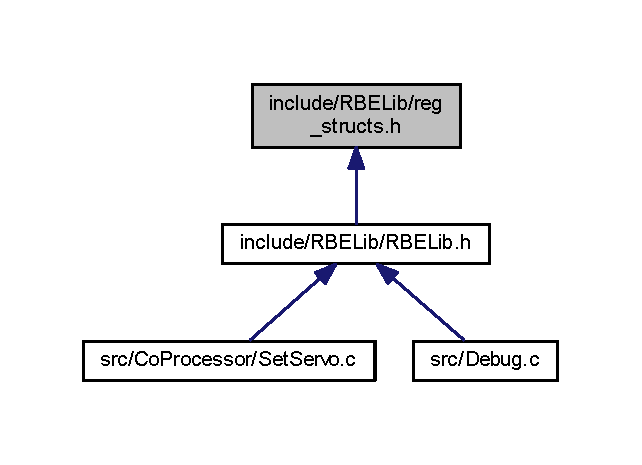
\includegraphics[width=308pt]{reg__structs_8h__dep__incl}
\end{center}
\end{figure}
\subsection*{Data Structures}
\begin{DoxyCompactItemize}
\item 
struct \hyperlink{struct____8bitreg__t}{\-\_\-\-\_\-8bitreg\-\_\-t}
\begin{DoxyCompactList}\small\item\em Generic byte register. \end{DoxyCompactList}\item 
struct \hyperlink{struct_____s_p_i_p_o_r_tbits__t}{\-\_\-\-\_\-\-S\-P\-I\-P\-O\-R\-Tbits\-\_\-t}
\begin{DoxyCompactList}\small\item\em S\-P\-I port. \end{DoxyCompactList}\end{DoxyCompactItemize}
\subsection*{Functions}
\begin{DoxyCompactItemize}
\item 
volatile \hyperlink{struct____8bitreg__t}{\-\_\-\-\_\-8bitreg\-\_\-t} P\-I\-N\-Abits \hyperlink{reg__structs_8h_ad6e205a0310f0e86e8681e9aaab5fbca}{\-\_\-\-\_\-asm\-\_\-\-\_\-} (\char`\"{}0x20\char`\"{}) \-\_\-\-\_\-attribute\-\_\-\-\_\-((section(\char`\"{}sfr\char`\"{})))
\item 
volatile \hyperlink{struct____8bitreg__t}{\-\_\-\-\_\-8bitreg\-\_\-t} D\-D\-R\-Abits \hyperlink{reg__structs_8h_ac254b9b3060f51b614af5b02211be437}{\-\_\-\-\_\-asm\-\_\-\-\_\-} (\char`\"{}0x21\char`\"{}) \-\_\-\-\_\-attribute\-\_\-\-\_\-((section(\char`\"{}sfr\char`\"{})))
\item 
volatile \hyperlink{struct____8bitreg__t}{\-\_\-\-\_\-8bitreg\-\_\-t} P\-O\-R\-T\-Abits \hyperlink{reg__structs_8h_add00742401aeaffbf415c2490de21b79}{\-\_\-\-\_\-asm\-\_\-\-\_\-} (\char`\"{}0x22\char`\"{}) \-\_\-\-\_\-attribute\-\_\-\-\_\-((section(\char`\"{}sfr\char`\"{})))
\item 
volatile \hyperlink{struct____8bitreg__t}{\-\_\-\-\_\-8bitreg\-\_\-t} P\-I\-N\-Bbits \hyperlink{reg__structs_8h_a2cab06cafd8e4cc3f8ac8a8f00b348eb}{\-\_\-\-\_\-asm\-\_\-\-\_\-} (\char`\"{}0x23\char`\"{}) \-\_\-\-\_\-attribute\-\_\-\-\_\-((section(\char`\"{}sfr\char`\"{})))
\item 
volatile \hyperlink{struct____8bitreg__t}{\-\_\-\-\_\-8bitreg\-\_\-t} D\-D\-R\-Bbits \hyperlink{reg__structs_8h_a8e2fa6a92bab4d219b942f3c9757da11}{\-\_\-\-\_\-asm\-\_\-\-\_\-} (\char`\"{}0x24\char`\"{}) \-\_\-\-\_\-attribute\-\_\-\-\_\-((section(\char`\"{}sfr\char`\"{})))
\item 
volatile \hyperlink{struct____8bitreg__t}{\-\_\-\-\_\-8bitreg\-\_\-t} P\-O\-R\-T\-Bbits \hyperlink{reg__structs_8h_aefd503781828d2a4d9f5d81c4d31adc5}{\-\_\-\-\_\-asm\-\_\-\-\_\-} (\char`\"{}0x25\char`\"{}) \-\_\-\-\_\-attribute\-\_\-\-\_\-((section(\char`\"{}sfr\char`\"{})))
\item 
volatile \hyperlink{struct____8bitreg__t}{\-\_\-\-\_\-8bitreg\-\_\-t} P\-I\-N\-Cbits \hyperlink{reg__structs_8h_a32e9140350d7b847044ddb3719645307}{\-\_\-\-\_\-asm\-\_\-\-\_\-} (\char`\"{}0x26\char`\"{}) \-\_\-\-\_\-attribute\-\_\-\-\_\-((section(\char`\"{}sfr\char`\"{})))
\item 
volatile \hyperlink{struct____8bitreg__t}{\-\_\-\-\_\-8bitreg\-\_\-t} D\-D\-R\-Cbits \hyperlink{reg__structs_8h_af59ce364ffa5af95c7c426e37849b83e}{\-\_\-\-\_\-asm\-\_\-\-\_\-} (\char`\"{}0x27\char`\"{}) \-\_\-\-\_\-attribute\-\_\-\-\_\-((section(\char`\"{}sfr\char`\"{})))
\item 
volatile \hyperlink{struct____8bitreg__t}{\-\_\-\-\_\-8bitreg\-\_\-t} P\-O\-R\-T\-Cbits \hyperlink{reg__structs_8h_a1642f34d4bbcd37125c90ed0097cd28b}{\-\_\-\-\_\-asm\-\_\-\-\_\-} (\char`\"{}0x28\char`\"{}) \-\_\-\-\_\-attribute\-\_\-\-\_\-((section(\char`\"{}sfr\char`\"{})))
\item 
volatile \hyperlink{struct____8bitreg__t}{\-\_\-\-\_\-8bitreg\-\_\-t} P\-I\-N\-Dbits \hyperlink{reg__structs_8h_ae5b2690ca1b162c95ab5d8252163ade6}{\-\_\-\-\_\-asm\-\_\-\-\_\-} (\char`\"{}0x29\char`\"{}) \-\_\-\-\_\-attribute\-\_\-\-\_\-((section(\char`\"{}sfr\char`\"{})))
\item 
volatile \hyperlink{struct____8bitreg__t}{\-\_\-\-\_\-8bitreg\-\_\-t} D\-D\-R\-Dbits \hyperlink{reg__structs_8h_a19737fb82107205a5427c68239335949}{\-\_\-\-\_\-asm\-\_\-\-\_\-} (\char`\"{}0x2\-A\char`\"{}) \-\_\-\-\_\-attribute\-\_\-\-\_\-((section(\char`\"{}sfr\char`\"{})))
\item 
volatile \hyperlink{struct____8bitreg__t}{\-\_\-\-\_\-8bitreg\-\_\-t} P\-O\-R\-T\-Dbits \hyperlink{reg__structs_8h_aac911c9b739c0cd88146e5bad68922d1}{\-\_\-\-\_\-asm\-\_\-\-\_\-} (\char`\"{}0x2\-B\char`\"{}) \-\_\-\-\_\-attribute\-\_\-\-\_\-((section(\char`\"{}sfr\char`\"{})))
\end{DoxyCompactItemize}


\subsection{Detailed Description}
This file redefines some of the registers of the A\-Tmega644p as structs to allow for easy access to individual bit fields in each register. The general syntax is $<$register name$>$bits.\-\_\-$<$bitfield name$>$. \begin{DoxyAuthor}{Author}
Peter Alley 
\end{DoxyAuthor}
\begin{DoxyDate}{Date}
January 26, 2010
\end{DoxyDate}
\begin{DoxyAuthor}{Author}
Justin Barrett 
\end{DoxyAuthor}
\begin{DoxyDate}{Date}
August 23, 2011
\end{DoxyDate}
\begin{DoxyAuthor}{Author}
Eric Willcox 
\end{DoxyAuthor}
\begin{DoxyDate}{Date}
July 21, 2014 
\end{DoxyDate}


Definition in file \hyperlink{reg__structs_8h_source}{reg\-\_\-structs.\-h}.



\subsection{Function Documentation}
\hypertarget{reg__structs_8h_ad6e205a0310f0e86e8681e9aaab5fbca}{\index{reg\-\_\-structs.\-h@{reg\-\_\-structs.\-h}!\-\_\-\-\_\-asm\-\_\-\-\_\-@{\-\_\-\-\_\-asm\-\_\-\-\_\-}}
\index{\-\_\-\-\_\-asm\-\_\-\-\_\-@{\-\_\-\-\_\-asm\-\_\-\-\_\-}!reg_structs.h@{reg\-\_\-structs.\-h}}
\subsubsection[{\-\_\-\-\_\-asm\-\_\-\-\_\-}]{\setlength{\rightskip}{0pt plus 5cm}volatile {\bf \-\_\-\-\_\-8bitreg\-\_\-t} P\-I\-N\-Abits \-\_\-\-\_\-asm\-\_\-\-\_\- (
\begin{DoxyParamCaption}
\item[{\char`\"{}0x20\char`\"{}}]{}
\end{DoxyParamCaption}
)}}\label{reg__structs_8h_ad6e205a0310f0e86e8681e9aaab5fbca}
\hypertarget{reg__structs_8h_ac254b9b3060f51b614af5b02211be437}{\index{reg\-\_\-structs.\-h@{reg\-\_\-structs.\-h}!\-\_\-\-\_\-asm\-\_\-\-\_\-@{\-\_\-\-\_\-asm\-\_\-\-\_\-}}
\index{\-\_\-\-\_\-asm\-\_\-\-\_\-@{\-\_\-\-\_\-asm\-\_\-\-\_\-}!reg_structs.h@{reg\-\_\-structs.\-h}}
\subsubsection[{\-\_\-\-\_\-asm\-\_\-\-\_\-}]{\setlength{\rightskip}{0pt plus 5cm}volatile {\bf \-\_\-\-\_\-8bitreg\-\_\-t} D\-D\-R\-Abits \-\_\-\-\_\-asm\-\_\-\-\_\- (
\begin{DoxyParamCaption}
\item[{\char`\"{}0x21\char`\"{}}]{}
\end{DoxyParamCaption}
)}}\label{reg__structs_8h_ac254b9b3060f51b614af5b02211be437}
\hypertarget{reg__structs_8h_add00742401aeaffbf415c2490de21b79}{\index{reg\-\_\-structs.\-h@{reg\-\_\-structs.\-h}!\-\_\-\-\_\-asm\-\_\-\-\_\-@{\-\_\-\-\_\-asm\-\_\-\-\_\-}}
\index{\-\_\-\-\_\-asm\-\_\-\-\_\-@{\-\_\-\-\_\-asm\-\_\-\-\_\-}!reg_structs.h@{reg\-\_\-structs.\-h}}
\subsubsection[{\-\_\-\-\_\-asm\-\_\-\-\_\-}]{\setlength{\rightskip}{0pt plus 5cm}volatile {\bf \-\_\-\-\_\-8bitreg\-\_\-t} P\-O\-R\-T\-Abits \-\_\-\-\_\-asm\-\_\-\-\_\- (
\begin{DoxyParamCaption}
\item[{\char`\"{}0x22\char`\"{}}]{}
\end{DoxyParamCaption}
)}}\label{reg__structs_8h_add00742401aeaffbf415c2490de21b79}
\hypertarget{reg__structs_8h_a2cab06cafd8e4cc3f8ac8a8f00b348eb}{\index{reg\-\_\-structs.\-h@{reg\-\_\-structs.\-h}!\-\_\-\-\_\-asm\-\_\-\-\_\-@{\-\_\-\-\_\-asm\-\_\-\-\_\-}}
\index{\-\_\-\-\_\-asm\-\_\-\-\_\-@{\-\_\-\-\_\-asm\-\_\-\-\_\-}!reg_structs.h@{reg\-\_\-structs.\-h}}
\subsubsection[{\-\_\-\-\_\-asm\-\_\-\-\_\-}]{\setlength{\rightskip}{0pt plus 5cm}volatile {\bf \-\_\-\-\_\-8bitreg\-\_\-t} P\-I\-N\-Bbits \-\_\-\-\_\-asm\-\_\-\-\_\- (
\begin{DoxyParamCaption}
\item[{\char`\"{}0x23\char`\"{}}]{}
\end{DoxyParamCaption}
)}}\label{reg__structs_8h_a2cab06cafd8e4cc3f8ac8a8f00b348eb}
\hypertarget{reg__structs_8h_a8e2fa6a92bab4d219b942f3c9757da11}{\index{reg\-\_\-structs.\-h@{reg\-\_\-structs.\-h}!\-\_\-\-\_\-asm\-\_\-\-\_\-@{\-\_\-\-\_\-asm\-\_\-\-\_\-}}
\index{\-\_\-\-\_\-asm\-\_\-\-\_\-@{\-\_\-\-\_\-asm\-\_\-\-\_\-}!reg_structs.h@{reg\-\_\-structs.\-h}}
\subsubsection[{\-\_\-\-\_\-asm\-\_\-\-\_\-}]{\setlength{\rightskip}{0pt plus 5cm}volatile {\bf \-\_\-\-\_\-\-S\-P\-I\-P\-O\-R\-Tbits\-\_\-t} S\-P\-I\-D\-D\-Rbits \-\_\-\-\_\-asm\-\_\-\-\_\- (
\begin{DoxyParamCaption}
\item[{\char`\"{}0x24\char`\"{}}]{}
\end{DoxyParamCaption}
)}}\label{reg__structs_8h_a8e2fa6a92bab4d219b942f3c9757da11}
\hypertarget{reg__structs_8h_aefd503781828d2a4d9f5d81c4d31adc5}{\index{reg\-\_\-structs.\-h@{reg\-\_\-structs.\-h}!\-\_\-\-\_\-asm\-\_\-\-\_\-@{\-\_\-\-\_\-asm\-\_\-\-\_\-}}
\index{\-\_\-\-\_\-asm\-\_\-\-\_\-@{\-\_\-\-\_\-asm\-\_\-\-\_\-}!reg_structs.h@{reg\-\_\-structs.\-h}}
\subsubsection[{\-\_\-\-\_\-asm\-\_\-\-\_\-}]{\setlength{\rightskip}{0pt plus 5cm}volatile {\bf \-\_\-\-\_\-\-S\-P\-I\-P\-O\-R\-Tbits\-\_\-t} S\-P\-I\-P\-O\-R\-Tbits \-\_\-\-\_\-asm\-\_\-\-\_\- (
\begin{DoxyParamCaption}
\item[{\char`\"{}0x25\char`\"{}}]{}
\end{DoxyParamCaption}
)}}\label{reg__structs_8h_aefd503781828d2a4d9f5d81c4d31adc5}
\hypertarget{reg__structs_8h_a32e9140350d7b847044ddb3719645307}{\index{reg\-\_\-structs.\-h@{reg\-\_\-structs.\-h}!\-\_\-\-\_\-asm\-\_\-\-\_\-@{\-\_\-\-\_\-asm\-\_\-\-\_\-}}
\index{\-\_\-\-\_\-asm\-\_\-\-\_\-@{\-\_\-\-\_\-asm\-\_\-\-\_\-}!reg_structs.h@{reg\-\_\-structs.\-h}}
\subsubsection[{\-\_\-\-\_\-asm\-\_\-\-\_\-}]{\setlength{\rightskip}{0pt plus 5cm}volatile {\bf \-\_\-\-\_\-8bitreg\-\_\-t} P\-I\-N\-Cbits \-\_\-\-\_\-asm\-\_\-\-\_\- (
\begin{DoxyParamCaption}
\item[{\char`\"{}0x26\char`\"{}}]{}
\end{DoxyParamCaption}
)}}\label{reg__structs_8h_a32e9140350d7b847044ddb3719645307}
\hypertarget{reg__structs_8h_af59ce364ffa5af95c7c426e37849b83e}{\index{reg\-\_\-structs.\-h@{reg\-\_\-structs.\-h}!\-\_\-\-\_\-asm\-\_\-\-\_\-@{\-\_\-\-\_\-asm\-\_\-\-\_\-}}
\index{\-\_\-\-\_\-asm\-\_\-\-\_\-@{\-\_\-\-\_\-asm\-\_\-\-\_\-}!reg_structs.h@{reg\-\_\-structs.\-h}}
\subsubsection[{\-\_\-\-\_\-asm\-\_\-\-\_\-}]{\setlength{\rightskip}{0pt plus 5cm}volatile {\bf \-\_\-\-\_\-8bitreg\-\_\-t} D\-D\-R\-Cbits \-\_\-\-\_\-asm\-\_\-\-\_\- (
\begin{DoxyParamCaption}
\item[{\char`\"{}0x27\char`\"{}}]{}
\end{DoxyParamCaption}
)}}\label{reg__structs_8h_af59ce364ffa5af95c7c426e37849b83e}
\hypertarget{reg__structs_8h_a1642f34d4bbcd37125c90ed0097cd28b}{\index{reg\-\_\-structs.\-h@{reg\-\_\-structs.\-h}!\-\_\-\-\_\-asm\-\_\-\-\_\-@{\-\_\-\-\_\-asm\-\_\-\-\_\-}}
\index{\-\_\-\-\_\-asm\-\_\-\-\_\-@{\-\_\-\-\_\-asm\-\_\-\-\_\-}!reg_structs.h@{reg\-\_\-structs.\-h}}
\subsubsection[{\-\_\-\-\_\-asm\-\_\-\-\_\-}]{\setlength{\rightskip}{0pt plus 5cm}volatile {\bf \-\_\-\-\_\-8bitreg\-\_\-t} P\-O\-R\-T\-Cbits \-\_\-\-\_\-asm\-\_\-\-\_\- (
\begin{DoxyParamCaption}
\item[{\char`\"{}0x28\char`\"{}}]{}
\end{DoxyParamCaption}
)}}\label{reg__structs_8h_a1642f34d4bbcd37125c90ed0097cd28b}
\hypertarget{reg__structs_8h_ae5b2690ca1b162c95ab5d8252163ade6}{\index{reg\-\_\-structs.\-h@{reg\-\_\-structs.\-h}!\-\_\-\-\_\-asm\-\_\-\-\_\-@{\-\_\-\-\_\-asm\-\_\-\-\_\-}}
\index{\-\_\-\-\_\-asm\-\_\-\-\_\-@{\-\_\-\-\_\-asm\-\_\-\-\_\-}!reg_structs.h@{reg\-\_\-structs.\-h}}
\subsubsection[{\-\_\-\-\_\-asm\-\_\-\-\_\-}]{\setlength{\rightskip}{0pt plus 5cm}volatile {\bf \-\_\-\-\_\-8bitreg\-\_\-t} P\-I\-N\-Dbits \-\_\-\-\_\-asm\-\_\-\-\_\- (
\begin{DoxyParamCaption}
\item[{\char`\"{}0x29\char`\"{}}]{}
\end{DoxyParamCaption}
)}}\label{reg__structs_8h_ae5b2690ca1b162c95ab5d8252163ade6}
\hypertarget{reg__structs_8h_a19737fb82107205a5427c68239335949}{\index{reg\-\_\-structs.\-h@{reg\-\_\-structs.\-h}!\-\_\-\-\_\-asm\-\_\-\-\_\-@{\-\_\-\-\_\-asm\-\_\-\-\_\-}}
\index{\-\_\-\-\_\-asm\-\_\-\-\_\-@{\-\_\-\-\_\-asm\-\_\-\-\_\-}!reg_structs.h@{reg\-\_\-structs.\-h}}
\subsubsection[{\-\_\-\-\_\-asm\-\_\-\-\_\-}]{\setlength{\rightskip}{0pt plus 5cm}volatile {\bf \-\_\-\-\_\-8bitreg\-\_\-t} D\-D\-R\-Dbits \-\_\-\-\_\-asm\-\_\-\-\_\- (
\begin{DoxyParamCaption}
\item[{\char`\"{}0x2\-A\char`\"{}}]{}
\end{DoxyParamCaption}
)}}\label{reg__structs_8h_a19737fb82107205a5427c68239335949}
\hypertarget{reg__structs_8h_aac911c9b739c0cd88146e5bad68922d1}{\index{reg\-\_\-structs.\-h@{reg\-\_\-structs.\-h}!\-\_\-\-\_\-asm\-\_\-\-\_\-@{\-\_\-\-\_\-asm\-\_\-\-\_\-}}
\index{\-\_\-\-\_\-asm\-\_\-\-\_\-@{\-\_\-\-\_\-asm\-\_\-\-\_\-}!reg_structs.h@{reg\-\_\-structs.\-h}}
\subsubsection[{\-\_\-\-\_\-asm\-\_\-\-\_\-}]{\setlength{\rightskip}{0pt plus 5cm}volatile {\bf \-\_\-\-\_\-8bitreg\-\_\-t} P\-O\-R\-T\-Dbits \-\_\-\-\_\-asm\-\_\-\-\_\- (
\begin{DoxyParamCaption}
\item[{\char`\"{}0x2\-B\char`\"{}}]{}
\end{DoxyParamCaption}
)}}\label{reg__structs_8h_aac911c9b739c0cd88146e5bad68922d1}

\hypertarget{_set_servo_8h}{\section{include/\-R\-B\-E\-Lib/\-Set\-Servo.h File Reference}
\label{_set_servo_8h}\index{include/\-R\-B\-E\-Lib/\-Set\-Servo.\-h@{include/\-R\-B\-E\-Lib/\-Set\-Servo.\-h}}
}


This file allows for using the Ser\-Sevo function to move the conveyor and gripper.  


This graph shows which files directly or indirectly include this file\-:\nopagebreak
\begin{figure}[H]
\begin{center}
\leavevmode
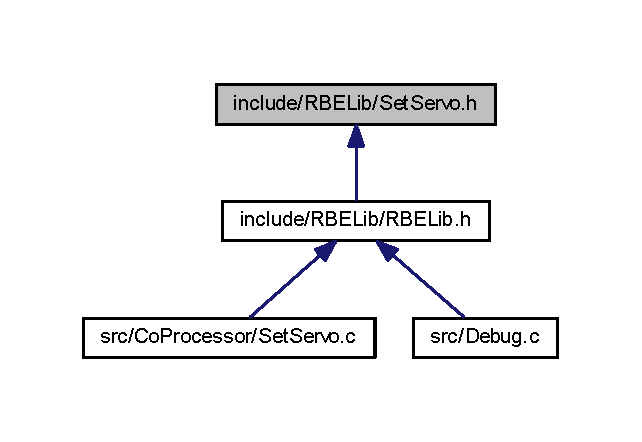
\includegraphics[width=308pt]{_set_servo_8h__dep__incl}
\end{center}
\end{figure}
\subsection*{Macros}
\begin{DoxyCompactItemize}
\item 
\#define \hyperlink{_set_servo_8h_a4b355291fe6b8ba8e167ab0faa862e45}{C\-L\-K}~18432000
\end{DoxyCompactItemize}
\subsection*{Functions}
\begin{DoxyCompactItemize}
\item 
void \hyperlink{_set_servo_8h_aacba653c33e27af6b2ea227100a4217b}{set\-Servo} (int Pin, int Value)
\begin{DoxyCompactList}\small\item\em Set a servo to a desired value. \end{DoxyCompactList}\item 
void \hyperlink{_set_servo_8h_acf43396e8eedf7c983cb59202c5af432}{init\-Alt\-Com} (unsigned long baudrate)
\begin{DoxyCompactList}\small\item\em Used to initialize U\-A\-R\-T0 for communication with the coprocessor. It should never be called manually. \end{DoxyCompactList}\item 
void \hyperlink{_set_servo_8h_a7bf02a3a3e6ee16ae38c3a03bf028023}{set\-Char\-Debug} (char byte\-To\-Send)
\begin{DoxyCompactList}\small\item\em Used to put a char on U\-A\-R\-T0. It should never be called manually and is used by printf(). \end{DoxyCompactList}\item 
void \hyperlink{_set_servo_8h_a3d09a92ac746ecc79b3b6b107357853b}{co\-Printf} (char $\ast$str)
\begin{DoxyCompactList}\small\item\em String to send to the coprocessor via U\-A\-R\-T0. \end{DoxyCompactList}\end{DoxyCompactItemize}


\subsection{Detailed Description}
This file allows for using the Ser\-Sevo function to move the conveyor and gripper. \begin{DoxyAuthor}{Author}
cwrus 
\end{DoxyAuthor}
\begin{DoxyDate}{Date}
Jun 28, 2012
\end{DoxyDate}
\begin{DoxyAuthor}{Author}
Eric Willcox 
\end{DoxyAuthor}
\begin{DoxyDate}{Date}
July 9, 2014 
\end{DoxyDate}


Definition in file \hyperlink{_set_servo_8h_source}{Set\-Servo.\-h}.



\subsection{Macro Definition Documentation}
\hypertarget{_set_servo_8h_a4b355291fe6b8ba8e167ab0faa862e45}{\index{Set\-Servo.\-h@{Set\-Servo.\-h}!C\-L\-K@{C\-L\-K}}
\index{C\-L\-K@{C\-L\-K}!SetServo.h@{Set\-Servo.\-h}}
\subsubsection[{C\-L\-K}]{\setlength{\rightskip}{0pt plus 5cm}\#define C\-L\-K~18432000}}\label{_set_servo_8h_a4b355291fe6b8ba8e167ab0faa862e45}


Definition at line 16 of file Set\-Servo.\-h.



Referenced by init\-Alt\-Com().



\subsection{Function Documentation}
\hypertarget{_set_servo_8h_a3d09a92ac746ecc79b3b6b107357853b}{\index{Set\-Servo.\-h@{Set\-Servo.\-h}!co\-Printf@{co\-Printf}}
\index{co\-Printf@{co\-Printf}!SetServo.h@{Set\-Servo.\-h}}
\subsubsection[{co\-Printf}]{\setlength{\rightskip}{0pt plus 5cm}void co\-Printf (
\begin{DoxyParamCaption}
\item[{char $\ast$}]{str}
\end{DoxyParamCaption}
)}}\label{_set_servo_8h_a3d09a92ac746ecc79b3b6b107357853b}


String to send to the coprocessor via U\-A\-R\-T0. 


\begin{DoxyParams}{Parameters}
{\em $\ast$str} & String to send. \\
\hline
\end{DoxyParams}


Definition at line 71 of file Set\-Servo.\-c.



References set\-Char\-Debug().



Referenced by set\-Servo().



Here is the call graph for this function\-:\nopagebreak
\begin{figure}[H]
\begin{center}
\leavevmode
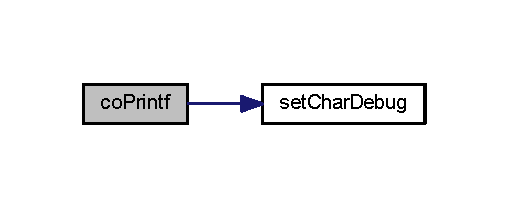
\includegraphics[width=244pt]{_set_servo_8h_a3d09a92ac746ecc79b3b6b107357853b_cgraph}
\end{center}
\end{figure}


\hypertarget{_set_servo_8h_acf43396e8eedf7c983cb59202c5af432}{\index{Set\-Servo.\-h@{Set\-Servo.\-h}!init\-Alt\-Com@{init\-Alt\-Com}}
\index{init\-Alt\-Com@{init\-Alt\-Com}!SetServo.h@{Set\-Servo.\-h}}
\subsubsection[{init\-Alt\-Com}]{\setlength{\rightskip}{0pt plus 5cm}void init\-Alt\-Com (
\begin{DoxyParamCaption}
\item[{unsigned long}]{baudrate}
\end{DoxyParamCaption}
)}}\label{_set_servo_8h_acf43396e8eedf7c983cb59202c5af432}


Used to initialize U\-A\-R\-T0 for communication with the coprocessor. It should never be called manually. 


\begin{DoxyParams}{Parameters}
{\em baudrate} & Baud rate of the communication line in bps. \\
\hline
\end{DoxyParams}


Definition at line 28 of file Set\-Servo.\-c.



References C\-L\-K.



Referenced by init\-R\-B\-E\-Lib().

\hypertarget{_set_servo_8h_a7bf02a3a3e6ee16ae38c3a03bf028023}{\index{Set\-Servo.\-h@{Set\-Servo.\-h}!set\-Char\-Debug@{set\-Char\-Debug}}
\index{set\-Char\-Debug@{set\-Char\-Debug}!SetServo.h@{Set\-Servo.\-h}}
\subsubsection[{set\-Char\-Debug}]{\setlength{\rightskip}{0pt plus 5cm}void set\-Char\-Debug (
\begin{DoxyParamCaption}
\item[{char}]{byte\-To\-Send}
\end{DoxyParamCaption}
)}}\label{_set_servo_8h_a7bf02a3a3e6ee16ae38c3a03bf028023}


Used to put a char on U\-A\-R\-T0. It should never be called manually and is used by printf(). 


\begin{DoxyParams}{Parameters}
{\em byte\-To\-Send} & Character to send \\
\hline
\end{DoxyParams}


Definition at line 57 of file Set\-Servo.\-c.



Referenced by co\-Printf().

\hypertarget{_set_servo_8h_aacba653c33e27af6b2ea227100a4217b}{\index{Set\-Servo.\-h@{Set\-Servo.\-h}!set\-Servo@{set\-Servo}}
\index{set\-Servo@{set\-Servo}!SetServo.h@{Set\-Servo.\-h}}
\subsubsection[{set\-Servo}]{\setlength{\rightskip}{0pt plus 5cm}void set\-Servo (
\begin{DoxyParamCaption}
\item[{int}]{Pin, }
\item[{int}]{Value}
\end{DoxyParamCaption}
)}}\label{_set_servo_8h_aacba653c33e27af6b2ea227100a4217b}


Set a servo to a desired value. 


\begin{DoxyParams}{Parameters}
{\em Pin} & Pin number. \\
\hline
{\em Value} & Value to set the pin to. \\
\hline
\end{DoxyParams}


Definition at line 17 of file Set\-Servo.\-c.



References co\-Printf().



Here is the call graph for this function\-:\nopagebreak
\begin{figure}[H]
\begin{center}
\leavevmode
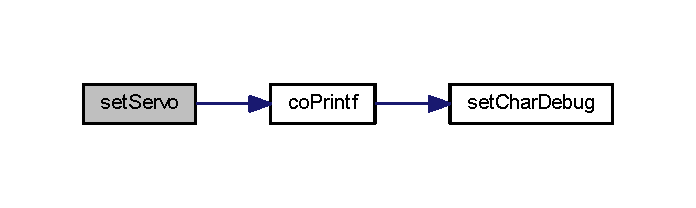
\includegraphics[width=334pt]{_set_servo_8h_aacba653c33e27af6b2ea227100a4217b_cgraph}
\end{center}
\end{figure}



\hypertarget{_slave_selects_8h}{\section{include/\-R\-B\-E\-Lib/\-Slave\-Selects.h File Reference}
\label{_slave_selects_8h}\index{include/\-R\-B\-E\-Lib/\-Slave\-Selects.\-h@{include/\-R\-B\-E\-Lib/\-Slave\-Selects.\-h}}
}


Here are all of the S\-P\-I line constants such as select lines and direction registers that can be called easily by the user instead of looking up the pins manually.  


{\ttfamily \#include \char`\"{}ports.\-h\char`\"{}}\\*
Include dependency graph for Slave\-Selects.\-h\-:\nopagebreak
\begin{figure}[H]
\begin{center}
\leavevmode
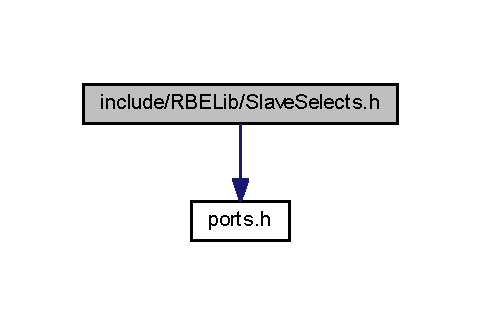
\includegraphics[width=231pt]{_slave_selects_8h__incl}
\end{center}
\end{figure}
This graph shows which files directly or indirectly include this file\-:\nopagebreak
\begin{figure}[H]
\begin{center}
\leavevmode
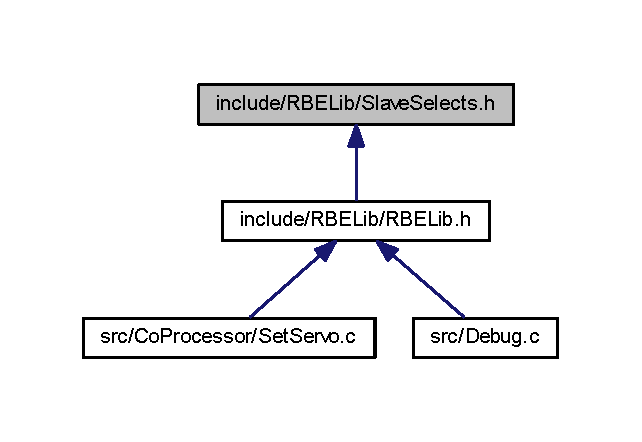
\includegraphics[width=308pt]{_slave_selects_8h__dep__incl}
\end{center}
\end{figure}
\subsection*{Macros}
\begin{DoxyCompactItemize}
\item 
\#define \hyperlink{_slave_selects_8h_ab142cc77dfa97010c9d2b616d0992b64}{S\-P\-I\-\_\-\-M\-I\-S\-O}~P\-O\-R\-T\-Bbits.\-\_\-\-P6
\begin{DoxyCompactList}\small\item\em S\-P\-I M\-I\-S\-O. \end{DoxyCompactList}\item 
\#define \hyperlink{_slave_selects_8h_a366f58da009f5d03b8753a41a5c57d84}{S\-P\-I\-\_\-\-M\-I\-S\-O\-\_\-\-D\-D\-R}~D\-D\-R\-Bbits.\-\_\-\-P6
\begin{DoxyCompactList}\small\item\em S\-P\-I M\-I\-S\-O. \end{DoxyCompactList}\item 
\#define \hyperlink{_slave_selects_8h_a7dbebab5f7dd57885adccf6711b13592}{S\-P\-I\-\_\-\-M\-O\-S\-I}~P\-O\-R\-T\-Bbits.\-\_\-\-P5
\begin{DoxyCompactList}\small\item\em S\-P\-I M\-O\-S\-I. \end{DoxyCompactList}\item 
\#define \hyperlink{_slave_selects_8h_af853ff26d66b9887d2212ef020cb22a4}{S\-P\-I\-\_\-\-M\-O\-S\-I\-\_\-\-D\-D\-R}~D\-D\-R\-Bbits.\-\_\-\-P5
\begin{DoxyCompactList}\small\item\em S\-P\-I M\-O\-S\-I. \end{DoxyCompactList}\item 
\#define \hyperlink{_slave_selects_8h_a750ca7c9b92cfc9e57272ff3a49db48b}{S\-P\-I\-\_\-\-S\-C\-K}~P\-O\-R\-T\-Bbits.\-\_\-\-P7
\begin{DoxyCompactList}\small\item\em S\-P\-I Clock. \end{DoxyCompactList}\item 
\#define \hyperlink{_slave_selects_8h_a5349415ea22a5febfe208e41e283e09e}{S\-P\-I\-\_\-\-S\-C\-K\-\_\-\-D\-D\-R}~D\-D\-R\-Bbits.\-\_\-\-P7
\begin{DoxyCompactList}\small\item\em S\-P\-I Clock. \end{DoxyCompactList}\item 
\#define \hyperlink{_slave_selects_8h_aec89105ab45250a756eb3d3638a4e92e}{S\-P\-I\-\_\-\-M\-A\-S\-T\-E\-R\-\_\-\-S\-S}~D\-D\-R\-Bbits.\-\_\-\-P4
\begin{DoxyCompactList}\small\item\em S\-P\-I master S\-S. \end{DoxyCompactList}\item 
\#define \hyperlink{_slave_selects_8h_ae1f19ab1d529611ee82a30686b31028e}{E\-N\-C\-O\-D\-E\-R\-\_\-\-S\-S\-\_\-0}~P\-O\-R\-T\-Cbits.\-\_\-\-P5
\begin{DoxyCompactList}\small\item\em S\-P\-I Slave Select Encoder 0. \end{DoxyCompactList}\item 
\#define \hyperlink{_slave_selects_8h_a9ab6d00d2ab688db5600737c60ddb314}{E\-N\-C\-O\-D\-E\-R\-\_\-\-S\-S\-\_\-1}~P\-O\-R\-T\-Cbits.\-\_\-\-P4
\begin{DoxyCompactList}\small\item\em S\-P\-I Slave Select Encoder 1. \end{DoxyCompactList}\item 
\#define \hyperlink{_slave_selects_8h_a203433243d028bc175021c37dc0802f6}{E\-N\-C\-O\-D\-E\-R\-\_\-\-S\-S\-\_\-2}~P\-O\-R\-T\-Cbits.\-\_\-\-P3
\begin{DoxyCompactList}\small\item\em S\-P\-I Slave Select Encoder 2. \end{DoxyCompactList}\item 
\#define \hyperlink{_slave_selects_8h_a086c9cf35f25608a5ff10bebea24a48c}{E\-N\-C\-O\-D\-E\-R\-\_\-\-S\-S\-\_\-3}~P\-O\-R\-T\-Cbits.\-\_\-\-P2
\begin{DoxyCompactList}\small\item\em S\-P\-I Slave Select Encoder 3. \end{DoxyCompactList}\item 
\#define \hyperlink{_slave_selects_8h_a7dbdb819db0851ee13ca6cbe1dc5f4c5}{D\-A\-C\-\_\-\-S\-S}~P\-O\-R\-T\-Dbits.\-\_\-\-P4
\begin{DoxyCompactList}\small\item\em S\-P\-I Slave Select D\-A\-C 1. \end{DoxyCompactList}\item 
\#define \hyperlink{_slave_selects_8h_ad742e387c55998038173396b907993a6}{A\-U\-X\-\_\-\-D\-A\-C\-\_\-\-S\-S}~P\-O\-R\-T\-Cbits.\-\_\-\-P6
\begin{DoxyCompactList}\small\item\em S\-P\-I Slave Select D\-A\-C 2. \end{DoxyCompactList}\item 
\#define \hyperlink{_slave_selects_8h_a34df7b0956f5a3b800db76cb529f13be}{E\-N\-C\-O\-D\-E\-R\-\_\-\-S\-S\-\_\-0\-\_\-ddr}~D\-D\-R\-Cbits.\-\_\-\-P5
\begin{DoxyCompactList}\small\item\em S\-P\-I Slave Select Encoder 0. \end{DoxyCompactList}\item 
\#define \hyperlink{_slave_selects_8h_aee3aa0c524fe3c2d1649afe3efd8cc72}{E\-N\-C\-O\-D\-E\-R\-\_\-\-S\-S\-\_\-1\-\_\-ddr}~D\-D\-R\-Cbits.\-\_\-\-P4
\begin{DoxyCompactList}\small\item\em S\-P\-I Slave Select Encoder 1. \end{DoxyCompactList}\item 
\#define \hyperlink{_slave_selects_8h_a742de3b51bc439fd401f864b1f3b91d1}{E\-N\-C\-O\-D\-E\-R\-\_\-\-S\-S\-\_\-2\-\_\-ddr}~D\-D\-R\-Cbits.\-\_\-\-P3
\begin{DoxyCompactList}\small\item\em S\-P\-I Slave Select Encoder 2. \end{DoxyCompactList}\item 
\#define \hyperlink{_slave_selects_8h_ab567f89cdb8e93ef39dac964fabcb085}{E\-N\-C\-O\-D\-E\-R\-\_\-\-S\-S\-\_\-3\-\_\-ddr}~D\-D\-R\-Cbits.\-\_\-\-P2
\begin{DoxyCompactList}\small\item\em S\-P\-I Slave Select Encoder 3. \end{DoxyCompactList}\item 
\#define \hyperlink{_slave_selects_8h_ae1575f1d0b95f42bc9011fadf88b80b6}{D\-A\-C\-\_\-\-S\-S\-\_\-ddr}~D\-D\-R\-Dbits.\-\_\-\-P4
\begin{DoxyCompactList}\small\item\em S\-P\-I Slave Select D\-A\-C 1. \end{DoxyCompactList}\item 
\#define \hyperlink{_slave_selects_8h_aa6a037d93a6cb48adee845861a4c866c}{A\-U\-X\-\_\-\-D\-A\-C\-\_\-\-S\-S\-\_\-ddr}~D\-D\-R\-Cbits.\-\_\-\-P6
\begin{DoxyCompactList}\small\item\em S\-P\-I Slave Select D\-A\-C 2. \end{DoxyCompactList}\item 
\#define \hyperlink{_slave_selects_8h_a427e16ab2edb4a8994821503d6991fb7}{S\-P\-A\-R\-E\-\_\-\-S\-S\-\_\-ddr}~D\-D\-R\-Cbits.\-\_\-\-P0
\begin{DoxyCompactList}\small\item\em S\-P\-I Slave Select Unused. \end{DoxyCompactList}\item 
\#define \hyperlink{_slave_selects_8h_a4148affed266edbb6bf487893da864d3}{E\-N\-C\-O\-D\-E\-R\-\_\-\-I\-R\-Q}~P\-O\-R\-T\-Bbitd.\-\_\-\-P2
\begin{DoxyCompactList}\small\item\em Interrupt line for all encoders. \end{DoxyCompactList}\item 
\#define \hyperlink{_slave_selects_8h_aedd2ac127b6656ad063c0970455e5497}{E\-N\-C\-O\-D\-E\-R\-\_\-\-I\-R\-Q\-\_\-ddr}~D\-D\-R\-Bbitd.\-\_\-\-P2
\begin{DoxyCompactList}\small\item\em Interrupt line for all encoders. \end{DoxyCompactList}\end{DoxyCompactItemize}


\subsection{Detailed Description}
Here are all of the S\-P\-I line constants such as select lines and direction registers that can be called easily by the user instead of looking up the pins manually. \begin{DoxyAuthor}{Author}
cwrus 
\end{DoxyAuthor}
\begin{DoxyDate}{Date}
Jun 28, 2012
\end{DoxyDate}
\begin{DoxyAuthor}{Author}
Eric Willcox 
\end{DoxyAuthor}
\begin{DoxyDate}{Date}
July 9, 2014 
\end{DoxyDate}


Definition in file \hyperlink{_slave_selects_8h_source}{Slave\-Selects.\-h}.



\subsection{Macro Definition Documentation}
\hypertarget{_slave_selects_8h_ad742e387c55998038173396b907993a6}{\index{Slave\-Selects.\-h@{Slave\-Selects.\-h}!A\-U\-X\-\_\-\-D\-A\-C\-\_\-\-S\-S@{A\-U\-X\-\_\-\-D\-A\-C\-\_\-\-S\-S}}
\index{A\-U\-X\-\_\-\-D\-A\-C\-\_\-\-S\-S@{A\-U\-X\-\_\-\-D\-A\-C\-\_\-\-S\-S}!SlaveSelects.h@{Slave\-Selects.\-h}}
\subsubsection[{A\-U\-X\-\_\-\-D\-A\-C\-\_\-\-S\-S}]{\setlength{\rightskip}{0pt plus 5cm}\#define A\-U\-X\-\_\-\-D\-A\-C\-\_\-\-S\-S~P\-O\-R\-T\-Cbits.\-\_\-\-P6}}\label{_slave_selects_8h_ad742e387c55998038173396b907993a6}


S\-P\-I Slave Select D\-A\-C 2. 



Definition at line 75 of file Slave\-Selects.\-h.

\hypertarget{_slave_selects_8h_aa6a037d93a6cb48adee845861a4c866c}{\index{Slave\-Selects.\-h@{Slave\-Selects.\-h}!A\-U\-X\-\_\-\-D\-A\-C\-\_\-\-S\-S\-\_\-ddr@{A\-U\-X\-\_\-\-D\-A\-C\-\_\-\-S\-S\-\_\-ddr}}
\index{A\-U\-X\-\_\-\-D\-A\-C\-\_\-\-S\-S\-\_\-ddr@{A\-U\-X\-\_\-\-D\-A\-C\-\_\-\-S\-S\-\_\-ddr}!SlaveSelects.h@{Slave\-Selects.\-h}}
\subsubsection[{A\-U\-X\-\_\-\-D\-A\-C\-\_\-\-S\-S\-\_\-ddr}]{\setlength{\rightskip}{0pt plus 5cm}\#define A\-U\-X\-\_\-\-D\-A\-C\-\_\-\-S\-S\-\_\-ddr~D\-D\-R\-Cbits.\-\_\-\-P6}}\label{_slave_selects_8h_aa6a037d93a6cb48adee845861a4c866c}


S\-P\-I Slave Select D\-A\-C 2. 



Definition at line 101 of file Slave\-Selects.\-h.

\hypertarget{_slave_selects_8h_a7dbdb819db0851ee13ca6cbe1dc5f4c5}{\index{Slave\-Selects.\-h@{Slave\-Selects.\-h}!D\-A\-C\-\_\-\-S\-S@{D\-A\-C\-\_\-\-S\-S}}
\index{D\-A\-C\-\_\-\-S\-S@{D\-A\-C\-\_\-\-S\-S}!SlaveSelects.h@{Slave\-Selects.\-h}}
\subsubsection[{D\-A\-C\-\_\-\-S\-S}]{\setlength{\rightskip}{0pt plus 5cm}\#define D\-A\-C\-\_\-\-S\-S~P\-O\-R\-T\-Dbits.\-\_\-\-P4}}\label{_slave_selects_8h_a7dbdb819db0851ee13ca6cbe1dc5f4c5}


S\-P\-I Slave Select D\-A\-C 1. 



Definition at line 71 of file Slave\-Selects.\-h.

\hypertarget{_slave_selects_8h_ae1575f1d0b95f42bc9011fadf88b80b6}{\index{Slave\-Selects.\-h@{Slave\-Selects.\-h}!D\-A\-C\-\_\-\-S\-S\-\_\-ddr@{D\-A\-C\-\_\-\-S\-S\-\_\-ddr}}
\index{D\-A\-C\-\_\-\-S\-S\-\_\-ddr@{D\-A\-C\-\_\-\-S\-S\-\_\-ddr}!SlaveSelects.h@{Slave\-Selects.\-h}}
\subsubsection[{D\-A\-C\-\_\-\-S\-S\-\_\-ddr}]{\setlength{\rightskip}{0pt plus 5cm}\#define D\-A\-C\-\_\-\-S\-S\-\_\-ddr~D\-D\-R\-Dbits.\-\_\-\-P4}}\label{_slave_selects_8h_ae1575f1d0b95f42bc9011fadf88b80b6}


S\-P\-I Slave Select D\-A\-C 1. 



Definition at line 97 of file Slave\-Selects.\-h.

\hypertarget{_slave_selects_8h_a4148affed266edbb6bf487893da864d3}{\index{Slave\-Selects.\-h@{Slave\-Selects.\-h}!E\-N\-C\-O\-D\-E\-R\-\_\-\-I\-R\-Q@{E\-N\-C\-O\-D\-E\-R\-\_\-\-I\-R\-Q}}
\index{E\-N\-C\-O\-D\-E\-R\-\_\-\-I\-R\-Q@{E\-N\-C\-O\-D\-E\-R\-\_\-\-I\-R\-Q}!SlaveSelects.h@{Slave\-Selects.\-h}}
\subsubsection[{E\-N\-C\-O\-D\-E\-R\-\_\-\-I\-R\-Q}]{\setlength{\rightskip}{0pt plus 5cm}\#define E\-N\-C\-O\-D\-E\-R\-\_\-\-I\-R\-Q~P\-O\-R\-T\-Bbitd.\-\_\-\-P2}}\label{_slave_selects_8h_a4148affed266edbb6bf487893da864d3}


Interrupt line for all encoders. 



Definition at line 110 of file Slave\-Selects.\-h.

\hypertarget{_slave_selects_8h_aedd2ac127b6656ad063c0970455e5497}{\index{Slave\-Selects.\-h@{Slave\-Selects.\-h}!E\-N\-C\-O\-D\-E\-R\-\_\-\-I\-R\-Q\-\_\-ddr@{E\-N\-C\-O\-D\-E\-R\-\_\-\-I\-R\-Q\-\_\-ddr}}
\index{E\-N\-C\-O\-D\-E\-R\-\_\-\-I\-R\-Q\-\_\-ddr@{E\-N\-C\-O\-D\-E\-R\-\_\-\-I\-R\-Q\-\_\-ddr}!SlaveSelects.h@{Slave\-Selects.\-h}}
\subsubsection[{E\-N\-C\-O\-D\-E\-R\-\_\-\-I\-R\-Q\-\_\-ddr}]{\setlength{\rightskip}{0pt plus 5cm}\#define E\-N\-C\-O\-D\-E\-R\-\_\-\-I\-R\-Q\-\_\-ddr~D\-D\-R\-Bbitd.\-\_\-\-P2}}\label{_slave_selects_8h_aedd2ac127b6656ad063c0970455e5497}


Interrupt line for all encoders. 



Definition at line 114 of file Slave\-Selects.\-h.

\hypertarget{_slave_selects_8h_ae1f19ab1d529611ee82a30686b31028e}{\index{Slave\-Selects.\-h@{Slave\-Selects.\-h}!E\-N\-C\-O\-D\-E\-R\-\_\-\-S\-S\-\_\-0@{E\-N\-C\-O\-D\-E\-R\-\_\-\-S\-S\-\_\-0}}
\index{E\-N\-C\-O\-D\-E\-R\-\_\-\-S\-S\-\_\-0@{E\-N\-C\-O\-D\-E\-R\-\_\-\-S\-S\-\_\-0}!SlaveSelects.h@{Slave\-Selects.\-h}}
\subsubsection[{E\-N\-C\-O\-D\-E\-R\-\_\-\-S\-S\-\_\-0}]{\setlength{\rightskip}{0pt plus 5cm}\#define E\-N\-C\-O\-D\-E\-R\-\_\-\-S\-S\-\_\-0~P\-O\-R\-T\-Cbits.\-\_\-\-P5}}\label{_slave_selects_8h_ae1f19ab1d529611ee82a30686b31028e}


S\-P\-I Slave Select Encoder 0. 



Definition at line 54 of file Slave\-Selects.\-h.

\hypertarget{_slave_selects_8h_a34df7b0956f5a3b800db76cb529f13be}{\index{Slave\-Selects.\-h@{Slave\-Selects.\-h}!E\-N\-C\-O\-D\-E\-R\-\_\-\-S\-S\-\_\-0\-\_\-ddr@{E\-N\-C\-O\-D\-E\-R\-\_\-\-S\-S\-\_\-0\-\_\-ddr}}
\index{E\-N\-C\-O\-D\-E\-R\-\_\-\-S\-S\-\_\-0\-\_\-ddr@{E\-N\-C\-O\-D\-E\-R\-\_\-\-S\-S\-\_\-0\-\_\-ddr}!SlaveSelects.h@{Slave\-Selects.\-h}}
\subsubsection[{E\-N\-C\-O\-D\-E\-R\-\_\-\-S\-S\-\_\-0\-\_\-ddr}]{\setlength{\rightskip}{0pt plus 5cm}\#define E\-N\-C\-O\-D\-E\-R\-\_\-\-S\-S\-\_\-0\-\_\-ddr~D\-D\-R\-Cbits.\-\_\-\-P5}}\label{_slave_selects_8h_a34df7b0956f5a3b800db76cb529f13be}


S\-P\-I Slave Select Encoder 0. 



Definition at line 80 of file Slave\-Selects.\-h.

\hypertarget{_slave_selects_8h_a9ab6d00d2ab688db5600737c60ddb314}{\index{Slave\-Selects.\-h@{Slave\-Selects.\-h}!E\-N\-C\-O\-D\-E\-R\-\_\-\-S\-S\-\_\-1@{E\-N\-C\-O\-D\-E\-R\-\_\-\-S\-S\-\_\-1}}
\index{E\-N\-C\-O\-D\-E\-R\-\_\-\-S\-S\-\_\-1@{E\-N\-C\-O\-D\-E\-R\-\_\-\-S\-S\-\_\-1}!SlaveSelects.h@{Slave\-Selects.\-h}}
\subsubsection[{E\-N\-C\-O\-D\-E\-R\-\_\-\-S\-S\-\_\-1}]{\setlength{\rightskip}{0pt plus 5cm}\#define E\-N\-C\-O\-D\-E\-R\-\_\-\-S\-S\-\_\-1~P\-O\-R\-T\-Cbits.\-\_\-\-P4}}\label{_slave_selects_8h_a9ab6d00d2ab688db5600737c60ddb314}


S\-P\-I Slave Select Encoder 1. 



Definition at line 58 of file Slave\-Selects.\-h.

\hypertarget{_slave_selects_8h_aee3aa0c524fe3c2d1649afe3efd8cc72}{\index{Slave\-Selects.\-h@{Slave\-Selects.\-h}!E\-N\-C\-O\-D\-E\-R\-\_\-\-S\-S\-\_\-1\-\_\-ddr@{E\-N\-C\-O\-D\-E\-R\-\_\-\-S\-S\-\_\-1\-\_\-ddr}}
\index{E\-N\-C\-O\-D\-E\-R\-\_\-\-S\-S\-\_\-1\-\_\-ddr@{E\-N\-C\-O\-D\-E\-R\-\_\-\-S\-S\-\_\-1\-\_\-ddr}!SlaveSelects.h@{Slave\-Selects.\-h}}
\subsubsection[{E\-N\-C\-O\-D\-E\-R\-\_\-\-S\-S\-\_\-1\-\_\-ddr}]{\setlength{\rightskip}{0pt plus 5cm}\#define E\-N\-C\-O\-D\-E\-R\-\_\-\-S\-S\-\_\-1\-\_\-ddr~D\-D\-R\-Cbits.\-\_\-\-P4}}\label{_slave_selects_8h_aee3aa0c524fe3c2d1649afe3efd8cc72}


S\-P\-I Slave Select Encoder 1. 



Definition at line 84 of file Slave\-Selects.\-h.

\hypertarget{_slave_selects_8h_a203433243d028bc175021c37dc0802f6}{\index{Slave\-Selects.\-h@{Slave\-Selects.\-h}!E\-N\-C\-O\-D\-E\-R\-\_\-\-S\-S\-\_\-2@{E\-N\-C\-O\-D\-E\-R\-\_\-\-S\-S\-\_\-2}}
\index{E\-N\-C\-O\-D\-E\-R\-\_\-\-S\-S\-\_\-2@{E\-N\-C\-O\-D\-E\-R\-\_\-\-S\-S\-\_\-2}!SlaveSelects.h@{Slave\-Selects.\-h}}
\subsubsection[{E\-N\-C\-O\-D\-E\-R\-\_\-\-S\-S\-\_\-2}]{\setlength{\rightskip}{0pt plus 5cm}\#define E\-N\-C\-O\-D\-E\-R\-\_\-\-S\-S\-\_\-2~P\-O\-R\-T\-Cbits.\-\_\-\-P3}}\label{_slave_selects_8h_a203433243d028bc175021c37dc0802f6}


S\-P\-I Slave Select Encoder 2. 



Definition at line 62 of file Slave\-Selects.\-h.

\hypertarget{_slave_selects_8h_a742de3b51bc439fd401f864b1f3b91d1}{\index{Slave\-Selects.\-h@{Slave\-Selects.\-h}!E\-N\-C\-O\-D\-E\-R\-\_\-\-S\-S\-\_\-2\-\_\-ddr@{E\-N\-C\-O\-D\-E\-R\-\_\-\-S\-S\-\_\-2\-\_\-ddr}}
\index{E\-N\-C\-O\-D\-E\-R\-\_\-\-S\-S\-\_\-2\-\_\-ddr@{E\-N\-C\-O\-D\-E\-R\-\_\-\-S\-S\-\_\-2\-\_\-ddr}!SlaveSelects.h@{Slave\-Selects.\-h}}
\subsubsection[{E\-N\-C\-O\-D\-E\-R\-\_\-\-S\-S\-\_\-2\-\_\-ddr}]{\setlength{\rightskip}{0pt plus 5cm}\#define E\-N\-C\-O\-D\-E\-R\-\_\-\-S\-S\-\_\-2\-\_\-ddr~D\-D\-R\-Cbits.\-\_\-\-P3}}\label{_slave_selects_8h_a742de3b51bc439fd401f864b1f3b91d1}


S\-P\-I Slave Select Encoder 2. 



Definition at line 88 of file Slave\-Selects.\-h.

\hypertarget{_slave_selects_8h_a086c9cf35f25608a5ff10bebea24a48c}{\index{Slave\-Selects.\-h@{Slave\-Selects.\-h}!E\-N\-C\-O\-D\-E\-R\-\_\-\-S\-S\-\_\-3@{E\-N\-C\-O\-D\-E\-R\-\_\-\-S\-S\-\_\-3}}
\index{E\-N\-C\-O\-D\-E\-R\-\_\-\-S\-S\-\_\-3@{E\-N\-C\-O\-D\-E\-R\-\_\-\-S\-S\-\_\-3}!SlaveSelects.h@{Slave\-Selects.\-h}}
\subsubsection[{E\-N\-C\-O\-D\-E\-R\-\_\-\-S\-S\-\_\-3}]{\setlength{\rightskip}{0pt plus 5cm}\#define E\-N\-C\-O\-D\-E\-R\-\_\-\-S\-S\-\_\-3~P\-O\-R\-T\-Cbits.\-\_\-\-P2}}\label{_slave_selects_8h_a086c9cf35f25608a5ff10bebea24a48c}


S\-P\-I Slave Select Encoder 3. 



Definition at line 66 of file Slave\-Selects.\-h.

\hypertarget{_slave_selects_8h_ab567f89cdb8e93ef39dac964fabcb085}{\index{Slave\-Selects.\-h@{Slave\-Selects.\-h}!E\-N\-C\-O\-D\-E\-R\-\_\-\-S\-S\-\_\-3\-\_\-ddr@{E\-N\-C\-O\-D\-E\-R\-\_\-\-S\-S\-\_\-3\-\_\-ddr}}
\index{E\-N\-C\-O\-D\-E\-R\-\_\-\-S\-S\-\_\-3\-\_\-ddr@{E\-N\-C\-O\-D\-E\-R\-\_\-\-S\-S\-\_\-3\-\_\-ddr}!SlaveSelects.h@{Slave\-Selects.\-h}}
\subsubsection[{E\-N\-C\-O\-D\-E\-R\-\_\-\-S\-S\-\_\-3\-\_\-ddr}]{\setlength{\rightskip}{0pt plus 5cm}\#define E\-N\-C\-O\-D\-E\-R\-\_\-\-S\-S\-\_\-3\-\_\-ddr~D\-D\-R\-Cbits.\-\_\-\-P2}}\label{_slave_selects_8h_ab567f89cdb8e93ef39dac964fabcb085}


S\-P\-I Slave Select Encoder 3. 



Definition at line 92 of file Slave\-Selects.\-h.

\hypertarget{_slave_selects_8h_a427e16ab2edb4a8994821503d6991fb7}{\index{Slave\-Selects.\-h@{Slave\-Selects.\-h}!S\-P\-A\-R\-E\-\_\-\-S\-S\-\_\-ddr@{S\-P\-A\-R\-E\-\_\-\-S\-S\-\_\-ddr}}
\index{S\-P\-A\-R\-E\-\_\-\-S\-S\-\_\-ddr@{S\-P\-A\-R\-E\-\_\-\-S\-S\-\_\-ddr}!SlaveSelects.h@{Slave\-Selects.\-h}}
\subsubsection[{S\-P\-A\-R\-E\-\_\-\-S\-S\-\_\-ddr}]{\setlength{\rightskip}{0pt plus 5cm}\#define S\-P\-A\-R\-E\-\_\-\-S\-S\-\_\-ddr~D\-D\-R\-Cbits.\-\_\-\-P0}}\label{_slave_selects_8h_a427e16ab2edb4a8994821503d6991fb7}


S\-P\-I Slave Select Unused. 



Definition at line 105 of file Slave\-Selects.\-h.

\hypertarget{_slave_selects_8h_aec89105ab45250a756eb3d3638a4e92e}{\index{Slave\-Selects.\-h@{Slave\-Selects.\-h}!S\-P\-I\-\_\-\-M\-A\-S\-T\-E\-R\-\_\-\-S\-S@{S\-P\-I\-\_\-\-M\-A\-S\-T\-E\-R\-\_\-\-S\-S}}
\index{S\-P\-I\-\_\-\-M\-A\-S\-T\-E\-R\-\_\-\-S\-S@{S\-P\-I\-\_\-\-M\-A\-S\-T\-E\-R\-\_\-\-S\-S}!SlaveSelects.h@{Slave\-Selects.\-h}}
\subsubsection[{S\-P\-I\-\_\-\-M\-A\-S\-T\-E\-R\-\_\-\-S\-S}]{\setlength{\rightskip}{0pt plus 5cm}\#define S\-P\-I\-\_\-\-M\-A\-S\-T\-E\-R\-\_\-\-S\-S~D\-D\-R\-Bbits.\-\_\-\-P4}}\label{_slave_selects_8h_aec89105ab45250a756eb3d3638a4e92e}


S\-P\-I master S\-S. 



Definition at line 50 of file Slave\-Selects.\-h.

\hypertarget{_slave_selects_8h_ab142cc77dfa97010c9d2b616d0992b64}{\index{Slave\-Selects.\-h@{Slave\-Selects.\-h}!S\-P\-I\-\_\-\-M\-I\-S\-O@{S\-P\-I\-\_\-\-M\-I\-S\-O}}
\index{S\-P\-I\-\_\-\-M\-I\-S\-O@{S\-P\-I\-\_\-\-M\-I\-S\-O}!SlaveSelects.h@{Slave\-Selects.\-h}}
\subsubsection[{S\-P\-I\-\_\-\-M\-I\-S\-O}]{\setlength{\rightskip}{0pt plus 5cm}\#define S\-P\-I\-\_\-\-M\-I\-S\-O~P\-O\-R\-T\-Bbits.\-\_\-\-P6}}\label{_slave_selects_8h_ab142cc77dfa97010c9d2b616d0992b64}


S\-P\-I M\-I\-S\-O. 



Definition at line 24 of file Slave\-Selects.\-h.

\hypertarget{_slave_selects_8h_a366f58da009f5d03b8753a41a5c57d84}{\index{Slave\-Selects.\-h@{Slave\-Selects.\-h}!S\-P\-I\-\_\-\-M\-I\-S\-O\-\_\-\-D\-D\-R@{S\-P\-I\-\_\-\-M\-I\-S\-O\-\_\-\-D\-D\-R}}
\index{S\-P\-I\-\_\-\-M\-I\-S\-O\-\_\-\-D\-D\-R@{S\-P\-I\-\_\-\-M\-I\-S\-O\-\_\-\-D\-D\-R}!SlaveSelects.h@{Slave\-Selects.\-h}}
\subsubsection[{S\-P\-I\-\_\-\-M\-I\-S\-O\-\_\-\-D\-D\-R}]{\setlength{\rightskip}{0pt plus 5cm}\#define S\-P\-I\-\_\-\-M\-I\-S\-O\-\_\-\-D\-D\-R~D\-D\-R\-Bbits.\-\_\-\-P6}}\label{_slave_selects_8h_a366f58da009f5d03b8753a41a5c57d84}


S\-P\-I M\-I\-S\-O. 



Definition at line 28 of file Slave\-Selects.\-h.

\hypertarget{_slave_selects_8h_a7dbebab5f7dd57885adccf6711b13592}{\index{Slave\-Selects.\-h@{Slave\-Selects.\-h}!S\-P\-I\-\_\-\-M\-O\-S\-I@{S\-P\-I\-\_\-\-M\-O\-S\-I}}
\index{S\-P\-I\-\_\-\-M\-O\-S\-I@{S\-P\-I\-\_\-\-M\-O\-S\-I}!SlaveSelects.h@{Slave\-Selects.\-h}}
\subsubsection[{S\-P\-I\-\_\-\-M\-O\-S\-I}]{\setlength{\rightskip}{0pt plus 5cm}\#define S\-P\-I\-\_\-\-M\-O\-S\-I~P\-O\-R\-T\-Bbits.\-\_\-\-P5}}\label{_slave_selects_8h_a7dbebab5f7dd57885adccf6711b13592}


S\-P\-I M\-O\-S\-I. 



Definition at line 33 of file Slave\-Selects.\-h.

\hypertarget{_slave_selects_8h_af853ff26d66b9887d2212ef020cb22a4}{\index{Slave\-Selects.\-h@{Slave\-Selects.\-h}!S\-P\-I\-\_\-\-M\-O\-S\-I\-\_\-\-D\-D\-R@{S\-P\-I\-\_\-\-M\-O\-S\-I\-\_\-\-D\-D\-R}}
\index{S\-P\-I\-\_\-\-M\-O\-S\-I\-\_\-\-D\-D\-R@{S\-P\-I\-\_\-\-M\-O\-S\-I\-\_\-\-D\-D\-R}!SlaveSelects.h@{Slave\-Selects.\-h}}
\subsubsection[{S\-P\-I\-\_\-\-M\-O\-S\-I\-\_\-\-D\-D\-R}]{\setlength{\rightskip}{0pt plus 5cm}\#define S\-P\-I\-\_\-\-M\-O\-S\-I\-\_\-\-D\-D\-R~D\-D\-R\-Bbits.\-\_\-\-P5}}\label{_slave_selects_8h_af853ff26d66b9887d2212ef020cb22a4}


S\-P\-I M\-O\-S\-I. 



Definition at line 37 of file Slave\-Selects.\-h.

\hypertarget{_slave_selects_8h_a750ca7c9b92cfc9e57272ff3a49db48b}{\index{Slave\-Selects.\-h@{Slave\-Selects.\-h}!S\-P\-I\-\_\-\-S\-C\-K@{S\-P\-I\-\_\-\-S\-C\-K}}
\index{S\-P\-I\-\_\-\-S\-C\-K@{S\-P\-I\-\_\-\-S\-C\-K}!SlaveSelects.h@{Slave\-Selects.\-h}}
\subsubsection[{S\-P\-I\-\_\-\-S\-C\-K}]{\setlength{\rightskip}{0pt plus 5cm}\#define S\-P\-I\-\_\-\-S\-C\-K~P\-O\-R\-T\-Bbits.\-\_\-\-P7}}\label{_slave_selects_8h_a750ca7c9b92cfc9e57272ff3a49db48b}


S\-P\-I Clock. 



Definition at line 42 of file Slave\-Selects.\-h.

\hypertarget{_slave_selects_8h_a5349415ea22a5febfe208e41e283e09e}{\index{Slave\-Selects.\-h@{Slave\-Selects.\-h}!S\-P\-I\-\_\-\-S\-C\-K\-\_\-\-D\-D\-R@{S\-P\-I\-\_\-\-S\-C\-K\-\_\-\-D\-D\-R}}
\index{S\-P\-I\-\_\-\-S\-C\-K\-\_\-\-D\-D\-R@{S\-P\-I\-\_\-\-S\-C\-K\-\_\-\-D\-D\-R}!SlaveSelects.h@{Slave\-Selects.\-h}}
\subsubsection[{S\-P\-I\-\_\-\-S\-C\-K\-\_\-\-D\-D\-R}]{\setlength{\rightskip}{0pt plus 5cm}\#define S\-P\-I\-\_\-\-S\-C\-K\-\_\-\-D\-D\-R~D\-D\-R\-Bbits.\-\_\-\-P7}}\label{_slave_selects_8h_a5349415ea22a5febfe208e41e283e09e}


S\-P\-I Clock. 



Definition at line 46 of file Slave\-Selects.\-h.


\hypertarget{_s_p_i_8h}{\section{include/\-R\-B\-E\-Lib/\-S\-P\-I.h File Reference}
\label{_s_p_i_8h}\index{include/\-R\-B\-E\-Lib/\-S\-P\-I.\-h@{include/\-R\-B\-E\-Lib/\-S\-P\-I.\-h}}
}


The header file and function prototypes for the S\-P\-I.  


This graph shows which files directly or indirectly include this file\-:\nopagebreak
\begin{figure}[H]
\begin{center}
\leavevmode
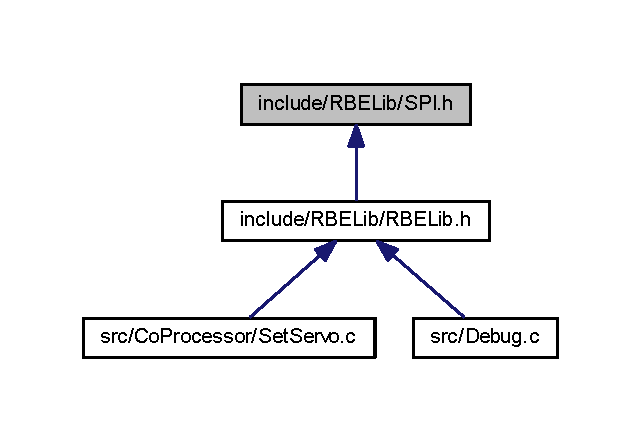
\includegraphics[width=308pt]{_s_p_i_8h__dep__incl}
\end{center}
\end{figure}
\subsection*{Functions}
\begin{DoxyCompactItemize}
\item 
void \hyperlink{_s_p_i_8h_a070402cc6c1cae693d10f59f9c483f76}{init\-S\-P\-I} ()
\begin{DoxyCompactList}\small\item\em Initializes the S\-P\-I bus for communication with all of your S\-P\-I devices. \end{DoxyCompactList}\item 
unsigned char \hyperlink{_s_p_i_8h_a4d2cd713b65091a59a9a2ee50b28bdf1}{spi\-Transceive} (\hyperlink{_r_b_e_lib_8h_aec93e83855ac17c3c25c55c37ca186dd}{B\-Y\-T\-E} data)
\begin{DoxyCompactList}\small\item\em Send and receive a byte out of the M\-O\-S\-I line. \end{DoxyCompactList}\end{DoxyCompactItemize}


\subsection{Detailed Description}
The header file and function prototypes for the S\-P\-I. \begin{DoxyRefDesc}{Bug}
\item[\hyperlink{bug__bug000001}{Bug}]While not a bug, some students have problems with some of the S\-P\-I devices where their code will not work after they send a command. To fix this, you may have to toggle the S\-S line once after sending your command and then disable it once more. This is because some of the devices need the toggle to load the registers and then execute the command.\end{DoxyRefDesc}


\begin{DoxyRefDesc}{Bug}
\item[\hyperlink{bug__bug000002}{Bug}]While not a bug, the D\-A\-C S\-S may need to be toggled at startup. This is only something that matters during a soft reset but should be done anyway during your initialization for S\-P\-I.\end{DoxyRefDesc}


\begin{DoxyAuthor}{Author}
kamiro87 
\end{DoxyAuthor}
\begin{DoxyDate}{Date}
August 31, 2010
\end{DoxyDate}
\begin{DoxyAuthor}{Author}
Justin Barrett 
\end{DoxyAuthor}
\begin{DoxyDate}{Date}
August 23, 2011
\end{DoxyDate}
\begin{DoxyAuthor}{Author}
Eric Willcox 
\end{DoxyAuthor}
\begin{DoxyDate}{Date}
August 20, 2013 
\end{DoxyDate}


Definition in file \hyperlink{_s_p_i_8h_source}{S\-P\-I.\-h}.



\subsection{Function Documentation}
\hypertarget{_s_p_i_8h_a070402cc6c1cae693d10f59f9c483f76}{\index{S\-P\-I.\-h@{S\-P\-I.\-h}!init\-S\-P\-I@{init\-S\-P\-I}}
\index{init\-S\-P\-I@{init\-S\-P\-I}!SPI.h@{S\-P\-I.\-h}}
\subsubsection[{init\-S\-P\-I}]{\setlength{\rightskip}{0pt plus 5cm}void init\-S\-P\-I (
\begin{DoxyParamCaption}
{}
\end{DoxyParamCaption}
)}}\label{_s_p_i_8h_a070402cc6c1cae693d10f59f9c483f76}


Initializes the S\-P\-I bus for communication with all of your S\-P\-I devices. 

\begin{DoxyRefDesc}{Todo}
\item[\hyperlink{todo__todo000024}{Todo}]Create the function that will allow you to initialize the S\-P\-I in a mode compatible with all devices. Do not forget to deassert all of your S\-S lines! \end{DoxyRefDesc}
\hypertarget{_s_p_i_8h_a4d2cd713b65091a59a9a2ee50b28bdf1}{\index{S\-P\-I.\-h@{S\-P\-I.\-h}!spi\-Transceive@{spi\-Transceive}}
\index{spi\-Transceive@{spi\-Transceive}!SPI.h@{S\-P\-I.\-h}}
\subsubsection[{spi\-Transceive}]{\setlength{\rightskip}{0pt plus 5cm}unsigned char spi\-Transceive (
\begin{DoxyParamCaption}
\item[{{\bf B\-Y\-T\-E}}]{data}
\end{DoxyParamCaption}
)}}\label{_s_p_i_8h_a4d2cd713b65091a59a9a2ee50b28bdf1}


Send and receive a byte out of the M\-O\-S\-I line. 

Please note that even if you do not want to receive any data back from a S\-P\-I device, the S\-P\-I standard requires you still receive something back even if it is junk data.


\begin{DoxyParams}{Parameters}
{\em data} & The byte to send down the S\-P\-I bus. \\
\hline
\end{DoxyParams}
\begin{DoxyReturn}{Returns}
value The byte shifted in during transmit
\end{DoxyReturn}
\begin{DoxyRefDesc}{Todo}
\item[\hyperlink{todo__todo000025}{Todo}]Make a function that will send a byte of data through the S\-P\-I and return whatever was sent back. \end{DoxyRefDesc}

\hypertarget{timer_8h}{\section{include/\-R\-B\-E\-Lib/timer.h File Reference}
\label{timer_8h}\index{include/\-R\-B\-E\-Lib/timer.\-h@{include/\-R\-B\-E\-Lib/timer.\-h}}
}


The header file and function prototypes for Timers 0-\/2.  


This graph shows which files directly or indirectly include this file\-:\nopagebreak
\begin{figure}[H]
\begin{center}
\leavevmode
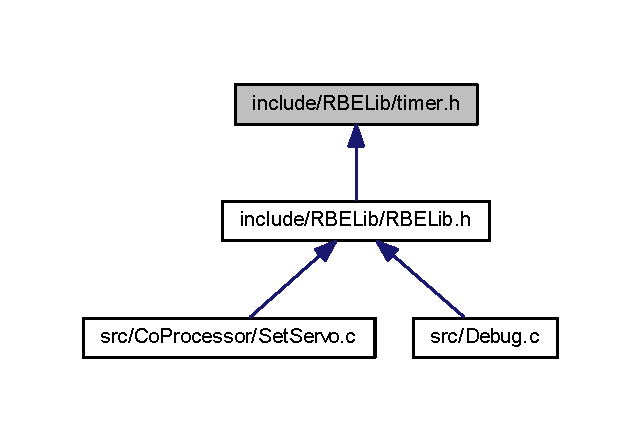
\includegraphics[width=308pt]{timer_8h__dep__incl}
\end{center}
\end{figure}
\subsection*{Macros}
\begin{DoxyCompactItemize}
\item 
\#define \hyperlink{timer_8h_a1291f416b069313021b519eea62d5bf1}{N\-O\-R\-M\-A\-L}~0
\begin{DoxyCompactList}\small\item\em Timer normal mode. \end{DoxyCompactList}\item 
\#define \hyperlink{timer_8h_ab51dc0e200a87209307849efeb202198}{C\-T\-C}~1
\begin{DoxyCompactList}\small\item\em Timer Clear Timer on Compare (C\-T\-C) mode. \end{DoxyCompactList}\end{DoxyCompactItemize}
\subsection*{Functions}
\begin{DoxyCompactItemize}
\item 
void \hyperlink{timer_8h_a467daa2177a6f16447a9ada6303c849a}{init\-Timer} (int timer, int mode, unsigned int comp)
\begin{DoxyCompactList}\small\item\em Initializes the specified timer in the specified mode. This header file provides constants for N\-O\-R\-M\-A\-L operation mode and C\-T\-C operation mode, however there are many more modes of operation for the Timers that can be experimented with. \end{DoxyCompactList}\item 
void \hyperlink{timer_8h_a7641a7bb79d647d59112ed4d20e01aeb}{set\-Comp\-Value} (unsigned char timer, unsigned short int comp)
\begin{DoxyCompactList}\small\item\em Only used when the specified timer is in C\-T\-C mode. Changes the value of the comparison register to the new specified value. \end{DoxyCompactList}\end{DoxyCompactItemize}


\subsection{Detailed Description}
The header file and function prototypes for Timers 0-\/2. \begin{DoxyAuthor}{Author}
Justin Barrett 
\end{DoxyAuthor}
\begin{DoxyDate}{Date}
August 25, 2011
\end{DoxyDate}
\begin{DoxyAuthor}{Author}
Eric Willcox 
\end{DoxyAuthor}
\begin{DoxyDate}{Date}
August 20, 2013 
\end{DoxyDate}


Definition in file \hyperlink{timer_8h_source}{timer.\-h}.



\subsection{Macro Definition Documentation}
\hypertarget{timer_8h_ab51dc0e200a87209307849efeb202198}{\index{timer.\-h@{timer.\-h}!C\-T\-C@{C\-T\-C}}
\index{C\-T\-C@{C\-T\-C}!timer.h@{timer.\-h}}
\subsubsection[{C\-T\-C}]{\setlength{\rightskip}{0pt plus 5cm}\#define C\-T\-C~1}}\label{timer_8h_ab51dc0e200a87209307849efeb202198}


Timer Clear Timer on Compare (C\-T\-C) mode. 



Definition at line 22 of file timer.\-h.

\hypertarget{timer_8h_a1291f416b069313021b519eea62d5bf1}{\index{timer.\-h@{timer.\-h}!N\-O\-R\-M\-A\-L@{N\-O\-R\-M\-A\-L}}
\index{N\-O\-R\-M\-A\-L@{N\-O\-R\-M\-A\-L}!timer.h@{timer.\-h}}
\subsubsection[{N\-O\-R\-M\-A\-L}]{\setlength{\rightskip}{0pt plus 5cm}\#define N\-O\-R\-M\-A\-L~0}}\label{timer_8h_a1291f416b069313021b519eea62d5bf1}


Timer normal mode. 



Definition at line 18 of file timer.\-h.



\subsection{Function Documentation}
\hypertarget{timer_8h_a467daa2177a6f16447a9ada6303c849a}{\index{timer.\-h@{timer.\-h}!init\-Timer@{init\-Timer}}
\index{init\-Timer@{init\-Timer}!timer.h@{timer.\-h}}
\subsubsection[{init\-Timer}]{\setlength{\rightskip}{0pt plus 5cm}void init\-Timer (
\begin{DoxyParamCaption}
\item[{int}]{timer, }
\item[{int}]{mode, }
\item[{unsigned int}]{comp}
\end{DoxyParamCaption}
)}}\label{timer_8h_a467daa2177a6f16447a9ada6303c849a}


Initializes the specified timer in the specified mode. This header file provides constants for N\-O\-R\-M\-A\-L operation mode and C\-T\-C operation mode, however there are many more modes of operation for the Timers that can be experimented with. 


\begin{DoxyParams}{Parameters}
{\em timer} & The number of the timer to be initialized (0-\/2). \\
\hline
{\em mode} & The mode to initialize the specified timer in. \\
\hline
{\em comp} & Only used in C\-T\-C mode. The value that the timer counts to before it triggers an interrupt and resets.\\
\hline
\end{DoxyParams}
\begin{DoxyRefDesc}{Todo}
\item[\hyperlink{todo__todo000026}{Todo}]Create a function that initializes the desired timer in a given mode and set the compare value (as appropriate). \end{DoxyRefDesc}
\hypertarget{timer_8h_a7641a7bb79d647d59112ed4d20e01aeb}{\index{timer.\-h@{timer.\-h}!set\-Comp\-Value@{set\-Comp\-Value}}
\index{set\-Comp\-Value@{set\-Comp\-Value}!timer.h@{timer.\-h}}
\subsubsection[{set\-Comp\-Value}]{\setlength{\rightskip}{0pt plus 5cm}void set\-Comp\-Value (
\begin{DoxyParamCaption}
\item[{unsigned char}]{timer, }
\item[{unsigned short int}]{comp}
\end{DoxyParamCaption}
)}}\label{timer_8h_a7641a7bb79d647d59112ed4d20e01aeb}


Only used when the specified timer is in C\-T\-C mode. Changes the value of the comparison register to the new specified value. 


\begin{DoxyParams}{Parameters}
{\em timer} & The timer comparison value to change (0-\/2). \\
\hline
{\em comp} & The value to set the comparison register to.\\
\hline
\end{DoxyParams}
\begin{DoxyRefDesc}{Todo}
\item[\hyperlink{todo__todo000027}{Todo}]Create a function that will set a new compare value for the given timer. \end{DoxyRefDesc}

\hypertarget{_u_s_a_r_t_debug_8h}{\section{include/\-R\-B\-E\-Lib/\-U\-S\-A\-R\-T\-Debug.h File Reference}
\label{_u_s_a_r_t_debug_8h}\index{include/\-R\-B\-E\-Lib/\-U\-S\-A\-R\-T\-Debug.\-h@{include/\-R\-B\-E\-Lib/\-U\-S\-A\-R\-T\-Debug.\-h}}
}


The header file and function prototypes for U\-S\-A\-R\-T1.  


This graph shows which files directly or indirectly include this file\-:\nopagebreak
\begin{figure}[H]
\begin{center}
\leavevmode
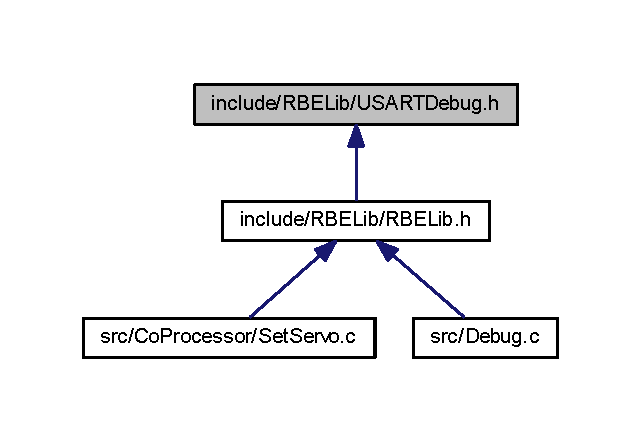
\includegraphics[width=308pt]{_u_s_a_r_t_debug_8h__dep__incl}
\end{center}
\end{figure}
\subsection*{Macros}
\begin{DoxyCompactItemize}
\item 
\#define \hyperlink{_u_s_a_r_t_debug_8h_ae9dc3b6e28948a9d8788412ce6a603cb}{D\-E\-F\-A\-U\-L\-T\-\_\-\-B\-A\-U\-D}~115200
\end{DoxyCompactItemize}
\subsection*{Functions}
\begin{DoxyCompactItemize}
\item 
void \hyperlink{_u_s_a_r_t_debug_8h_a9a96eb5e6b5a13fff8ed69716e76a314}{debug\-U\-S\-A\-R\-T\-Init} (unsigned long baudrate)
\begin{DoxyCompactList}\small\item\em Initializes U\-S\-A\-R\-T1 as a print terminal to the P\-C. This function must check the incoming baudrate against the valid baudrates from the data-\/sheet. If the baudrate is invalid, then the D\-E\-F\-A\-U\-L\-T\-\_\-\-B\-A\-U\-D constant must be used instead. \end{DoxyCompactList}\item 
void \hyperlink{_u_s_a_r_t_debug_8h_ab52220b9802762326175f5a6d09c50a1}{put\-Char\-Debug} (char byte\-To\-Send)
\begin{DoxyCompactList}\small\item\em Sends one byte to the U\-S\-A\-R\-T1 Tx pin (Transmits one byte). \end{DoxyCompactList}\item 
unsigned char \hyperlink{_u_s_a_r_t_debug_8h_aeaa27830bd87dcec2dd03213b02f22aa}{get\-Char\-Debug} (void)
\begin{DoxyCompactList}\small\item\em Recieves one byte of data from the serial port (i.\-e. from the P\-C). \end{DoxyCompactList}\end{DoxyCompactItemize}


\subsection{Detailed Description}
The header file and function prototypes for U\-S\-A\-R\-T1. \begin{DoxyAuthor}{Author}
Kevin Harrington 
\end{DoxyAuthor}
\begin{DoxyDate}{Date}
August 20, 2010
\end{DoxyDate}
\begin{DoxyAuthor}{Author}
Justin Barrett 
\end{DoxyAuthor}
\begin{DoxyDate}{Date}
August 25, 2011
\end{DoxyDate}
\begin{DoxyAuthor}{Author}
Eric Willcox 
\end{DoxyAuthor}
\begin{DoxyDate}{Date}
August 20, 2013 
\end{DoxyDate}


Definition in file \hyperlink{_u_s_a_r_t_debug_8h_source}{U\-S\-A\-R\-T\-Debug.\-h}.



\subsection{Macro Definition Documentation}
\hypertarget{_u_s_a_r_t_debug_8h_ae9dc3b6e28948a9d8788412ce6a603cb}{\index{U\-S\-A\-R\-T\-Debug.\-h@{U\-S\-A\-R\-T\-Debug.\-h}!D\-E\-F\-A\-U\-L\-T\-\_\-\-B\-A\-U\-D@{D\-E\-F\-A\-U\-L\-T\-\_\-\-B\-A\-U\-D}}
\index{D\-E\-F\-A\-U\-L\-T\-\_\-\-B\-A\-U\-D@{D\-E\-F\-A\-U\-L\-T\-\_\-\-B\-A\-U\-D}!USARTDebug.h@{U\-S\-A\-R\-T\-Debug.\-h}}
\subsubsection[{D\-E\-F\-A\-U\-L\-T\-\_\-\-B\-A\-U\-D}]{\setlength{\rightskip}{0pt plus 5cm}\#define D\-E\-F\-A\-U\-L\-T\-\_\-\-B\-A\-U\-D~115200}}\label{_u_s_a_r_t_debug_8h_ae9dc3b6e28948a9d8788412ce6a603cb}


Definition at line 19 of file U\-S\-A\-R\-T\-Debug.\-h.



\subsection{Function Documentation}
\hypertarget{_u_s_a_r_t_debug_8h_a9a96eb5e6b5a13fff8ed69716e76a314}{\index{U\-S\-A\-R\-T\-Debug.\-h@{U\-S\-A\-R\-T\-Debug.\-h}!debug\-U\-S\-A\-R\-T\-Init@{debug\-U\-S\-A\-R\-T\-Init}}
\index{debug\-U\-S\-A\-R\-T\-Init@{debug\-U\-S\-A\-R\-T\-Init}!USARTDebug.h@{U\-S\-A\-R\-T\-Debug.\-h}}
\subsubsection[{debug\-U\-S\-A\-R\-T\-Init}]{\setlength{\rightskip}{0pt plus 5cm}void debug\-U\-S\-A\-R\-T\-Init (
\begin{DoxyParamCaption}
\item[{unsigned long}]{baudrate}
\end{DoxyParamCaption}
)}}\label{_u_s_a_r_t_debug_8h_a9a96eb5e6b5a13fff8ed69716e76a314}


Initializes U\-S\-A\-R\-T1 as a print terminal to the P\-C. This function must check the incoming baudrate against the valid baudrates from the data-\/sheet. If the baudrate is invalid, then the D\-E\-F\-A\-U\-L\-T\-\_\-\-B\-A\-U\-D constant must be used instead. 


\begin{DoxyParams}{Parameters}
{\em baudrate} & The desired baudrate to set for U\-S\-A\-R\-T1.\\
\hline
\end{DoxyParams}
\begin{DoxyRefDesc}{Todo}
\item[\hyperlink{todo__todo000028}{Todo}]Create the function that will initialize U\-S\-A\-R\-T1 for debugging use. \end{DoxyRefDesc}
\hypertarget{_u_s_a_r_t_debug_8h_aeaa27830bd87dcec2dd03213b02f22aa}{\index{U\-S\-A\-R\-T\-Debug.\-h@{U\-S\-A\-R\-T\-Debug.\-h}!get\-Char\-Debug@{get\-Char\-Debug}}
\index{get\-Char\-Debug@{get\-Char\-Debug}!USARTDebug.h@{U\-S\-A\-R\-T\-Debug.\-h}}
\subsubsection[{get\-Char\-Debug}]{\setlength{\rightskip}{0pt plus 5cm}unsigned char get\-Char\-Debug (
\begin{DoxyParamCaption}
\item[{void}]{}
\end{DoxyParamCaption}
)}}\label{_u_s_a_r_t_debug_8h_aeaa27830bd87dcec2dd03213b02f22aa}


Recieves one byte of data from the serial port (i.\-e. from the P\-C). 

\begin{DoxyReturn}{Returns}
byte\-Received Character that was received on the U\-S\-A\-R\-T.
\end{DoxyReturn}
\begin{DoxyRefDesc}{Todo}
\item[\hyperlink{todo__todo000030}{Todo}]Make the function that will listen for input on the U\-S\-A\-R\-T1 R\-X line. \end{DoxyRefDesc}
\hypertarget{_u_s_a_r_t_debug_8h_ab52220b9802762326175f5a6d09c50a1}{\index{U\-S\-A\-R\-T\-Debug.\-h@{U\-S\-A\-R\-T\-Debug.\-h}!put\-Char\-Debug@{put\-Char\-Debug}}
\index{put\-Char\-Debug@{put\-Char\-Debug}!USARTDebug.h@{U\-S\-A\-R\-T\-Debug.\-h}}
\subsubsection[{put\-Char\-Debug}]{\setlength{\rightskip}{0pt plus 5cm}void put\-Char\-Debug (
\begin{DoxyParamCaption}
\item[{char}]{byte\-To\-Send}
\end{DoxyParamCaption}
)}}\label{_u_s_a_r_t_debug_8h_ab52220b9802762326175f5a6d09c50a1}


Sends one byte to the U\-S\-A\-R\-T1 Tx pin (Transmits one byte). 


\begin{DoxyParams}{Parameters}
{\em byte\-To\-Send} & The byte that is to be transmitted through U\-S\-A\-R\-T1.\\
\hline
\end{DoxyParams}
\begin{DoxyRefDesc}{Todo}
\item[\hyperlink{todo__todo000029}{Todo}]Make the function that will put a character on the U\-S\-A\-R\-T1 T\-X line. \end{DoxyRefDesc}


Referenced by printf\-R\-B\-E().


\hypertarget{_set_servo_8c}{\section{src/\-Co\-Processor/\-Set\-Servo.c File Reference}
\label{_set_servo_8c}\index{src/\-Co\-Processor/\-Set\-Servo.\-c@{src/\-Co\-Processor/\-Set\-Servo.\-c}}
}


Sending \hyperlink{_set_servo_8h_aacba653c33e27af6b2ea227100a4217b}{set\-Servo()} command to the coprocessor.  


{\ttfamily \#include \char`\"{}R\-B\-E\-Lib/\-R\-B\-E\-Lib.\-h\char`\"{}}\\*
Include dependency graph for Set\-Servo.\-c\-:\nopagebreak
\begin{figure}[H]
\begin{center}
\leavevmode
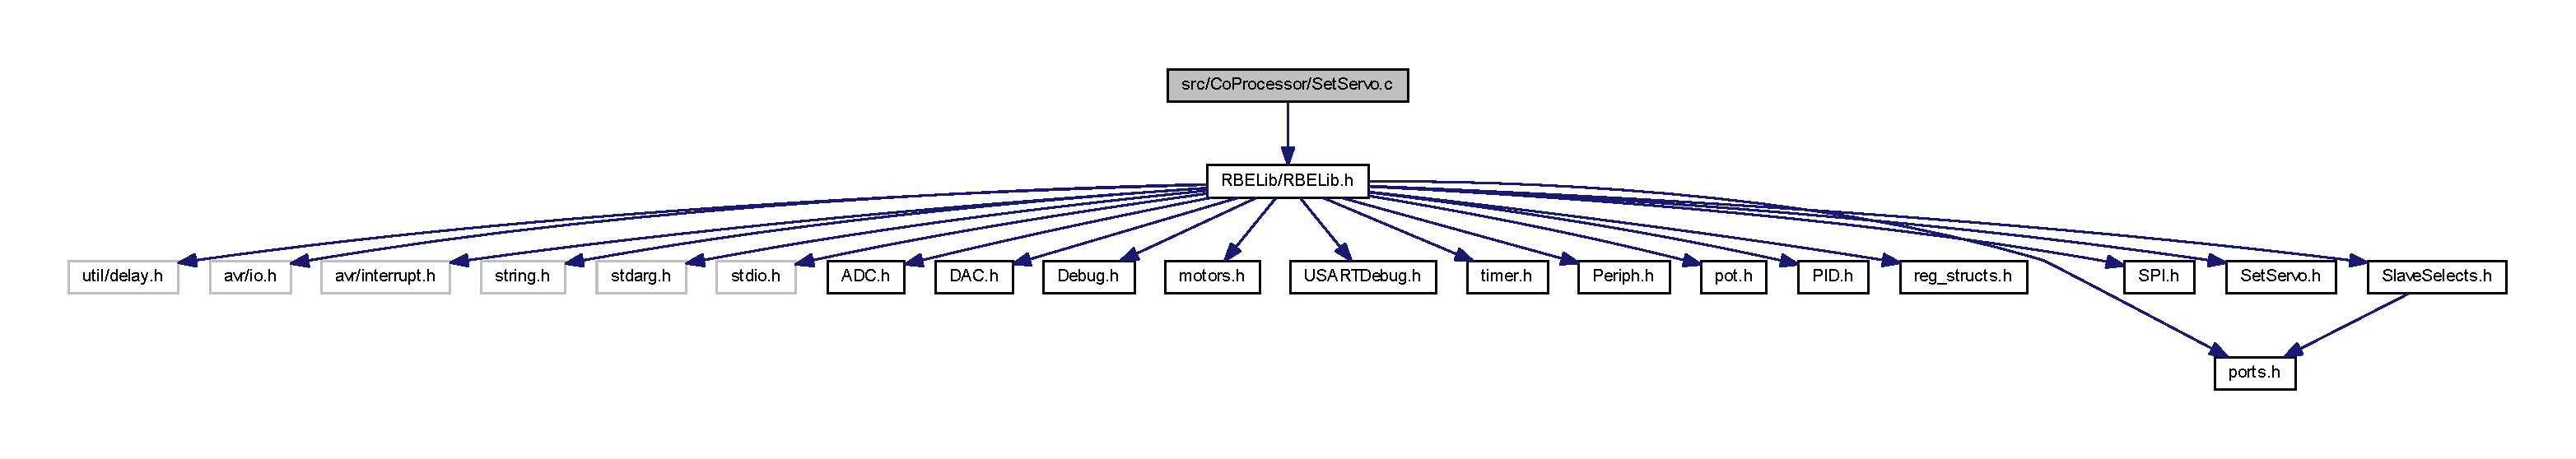
\includegraphics[width=350pt]{_set_servo_8c__incl}
\end{center}
\end{figure}
\subsection*{Functions}
\begin{DoxyCompactItemize}
\item 
void \hyperlink{_set_servo_8c_a3d1924bbf61ad71a669a1865f3a5ecd4}{set\-Servo} (int pin, int value)
\begin{DoxyCompactList}\small\item\em Set a servo to a desired value. \end{DoxyCompactList}\item 
void \hyperlink{_set_servo_8c_acf43396e8eedf7c983cb59202c5af432}{init\-Alt\-Com} (unsigned long baudrate)
\begin{DoxyCompactList}\small\item\em Used to initialize U\-A\-R\-T0 for communication with the coprocessor. It should never be called manually. \end{DoxyCompactList}\item 
void \hyperlink{_set_servo_8c_a7bf02a3a3e6ee16ae38c3a03bf028023}{set\-Char\-Debug} (char byte\-To\-Send)
\begin{DoxyCompactList}\small\item\em Used to put a char on U\-A\-R\-T0. It should never be called manually and is used by printf(). \end{DoxyCompactList}\item 
void \hyperlink{_set_servo_8c_a3d09a92ac746ecc79b3b6b107357853b}{co\-Printf} (char $\ast$str)
\begin{DoxyCompactList}\small\item\em String to send to the coprocessor via U\-A\-R\-T0. \end{DoxyCompactList}\end{DoxyCompactItemize}


\subsection{Detailed Description}
Sending \hyperlink{_set_servo_8h_aacba653c33e27af6b2ea227100a4217b}{set\-Servo()} command to the coprocessor. \begin{DoxyAuthor}{Author}
Eric Willcox 
\end{DoxyAuthor}
\begin{DoxyDate}{Date}
July 9, 2014 
\end{DoxyDate}


Definition in file \hyperlink{_set_servo_8c_source}{Set\-Servo.\-c}.



\subsection{Function Documentation}
\hypertarget{_set_servo_8c_a3d09a92ac746ecc79b3b6b107357853b}{\index{Set\-Servo.\-c@{Set\-Servo.\-c}!co\-Printf@{co\-Printf}}
\index{co\-Printf@{co\-Printf}!SetServo.c@{Set\-Servo.\-c}}
\subsubsection[{co\-Printf}]{\setlength{\rightskip}{0pt plus 5cm}void co\-Printf (
\begin{DoxyParamCaption}
\item[{char $\ast$}]{str}
\end{DoxyParamCaption}
)}}\label{_set_servo_8c_a3d09a92ac746ecc79b3b6b107357853b}


String to send to the coprocessor via U\-A\-R\-T0. 


\begin{DoxyParams}{Parameters}
{\em $\ast$str} & String to send. \\
\hline
\end{DoxyParams}


Definition at line 71 of file Set\-Servo.\-c.



References set\-Char\-Debug().



Referenced by set\-Servo().



Here is the call graph for this function\-:\nopagebreak
\begin{figure}[H]
\begin{center}
\leavevmode
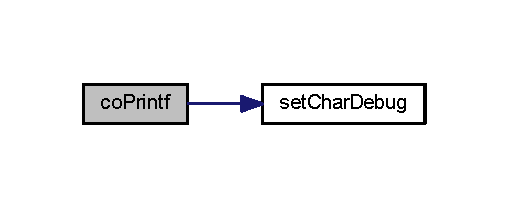
\includegraphics[width=244pt]{_set_servo_8c_a3d09a92ac746ecc79b3b6b107357853b_cgraph}
\end{center}
\end{figure}


\hypertarget{_set_servo_8c_acf43396e8eedf7c983cb59202c5af432}{\index{Set\-Servo.\-c@{Set\-Servo.\-c}!init\-Alt\-Com@{init\-Alt\-Com}}
\index{init\-Alt\-Com@{init\-Alt\-Com}!SetServo.c@{Set\-Servo.\-c}}
\subsubsection[{init\-Alt\-Com}]{\setlength{\rightskip}{0pt plus 5cm}void init\-Alt\-Com (
\begin{DoxyParamCaption}
\item[{unsigned long}]{baudrate}
\end{DoxyParamCaption}
)}}\label{_set_servo_8c_acf43396e8eedf7c983cb59202c5af432}


Used to initialize U\-A\-R\-T0 for communication with the coprocessor. It should never be called manually. 


\begin{DoxyParams}{Parameters}
{\em baudrate} & Baud rate of the communication line in bps. \\
\hline
\end{DoxyParams}


Definition at line 28 of file Set\-Servo.\-c.



References C\-L\-K.



Referenced by init\-R\-B\-E\-Lib().

\hypertarget{_set_servo_8c_a7bf02a3a3e6ee16ae38c3a03bf028023}{\index{Set\-Servo.\-c@{Set\-Servo.\-c}!set\-Char\-Debug@{set\-Char\-Debug}}
\index{set\-Char\-Debug@{set\-Char\-Debug}!SetServo.c@{Set\-Servo.\-c}}
\subsubsection[{set\-Char\-Debug}]{\setlength{\rightskip}{0pt plus 5cm}void set\-Char\-Debug (
\begin{DoxyParamCaption}
\item[{char}]{byte\-To\-Send}
\end{DoxyParamCaption}
)}}\label{_set_servo_8c_a7bf02a3a3e6ee16ae38c3a03bf028023}


Used to put a char on U\-A\-R\-T0. It should never be called manually and is used by printf(). 


\begin{DoxyParams}{Parameters}
{\em byte\-To\-Send} & Character to send \\
\hline
\end{DoxyParams}


Definition at line 57 of file Set\-Servo.\-c.



Referenced by co\-Printf().

\hypertarget{_set_servo_8c_a3d1924bbf61ad71a669a1865f3a5ecd4}{\index{Set\-Servo.\-c@{Set\-Servo.\-c}!set\-Servo@{set\-Servo}}
\index{set\-Servo@{set\-Servo}!SetServo.c@{Set\-Servo.\-c}}
\subsubsection[{set\-Servo}]{\setlength{\rightskip}{0pt plus 5cm}void set\-Servo (
\begin{DoxyParamCaption}
\item[{int}]{Pin, }
\item[{int}]{Value}
\end{DoxyParamCaption}
)}}\label{_set_servo_8c_a3d1924bbf61ad71a669a1865f3a5ecd4}


Set a servo to a desired value. 


\begin{DoxyParams}{Parameters}
{\em Pin} & Pin number. \\
\hline
{\em Value} & Value to set the pin to. \\
\hline
\end{DoxyParams}


Definition at line 17 of file Set\-Servo.\-c.



References co\-Printf().



Here is the call graph for this function\-:\nopagebreak
\begin{figure}[H]
\begin{center}
\leavevmode
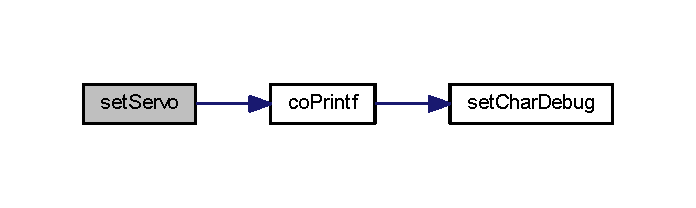
\includegraphics[width=334pt]{_set_servo_8c_a3d1924bbf61ad71a669a1865f3a5ecd4_cgraph}
\end{center}
\end{figure}



\hypertarget{_debug_8c}{\section{src/\-Debug.c File Reference}
\label{_debug_8c}\index{src/\-Debug.\-c@{src/\-Debug.\-c}}
}


Allows for printf() and \hyperlink{_set_servo_8h_aacba653c33e27af6b2ea227100a4217b}{set\-Servo()} capability.  


{\ttfamily \#include \char`\"{}R\-B\-E\-Lib/\-R\-B\-E\-Lib.\-h\char`\"{}}\\*
Include dependency graph for Debug.\-c\-:\nopagebreak
\begin{figure}[H]
\begin{center}
\leavevmode
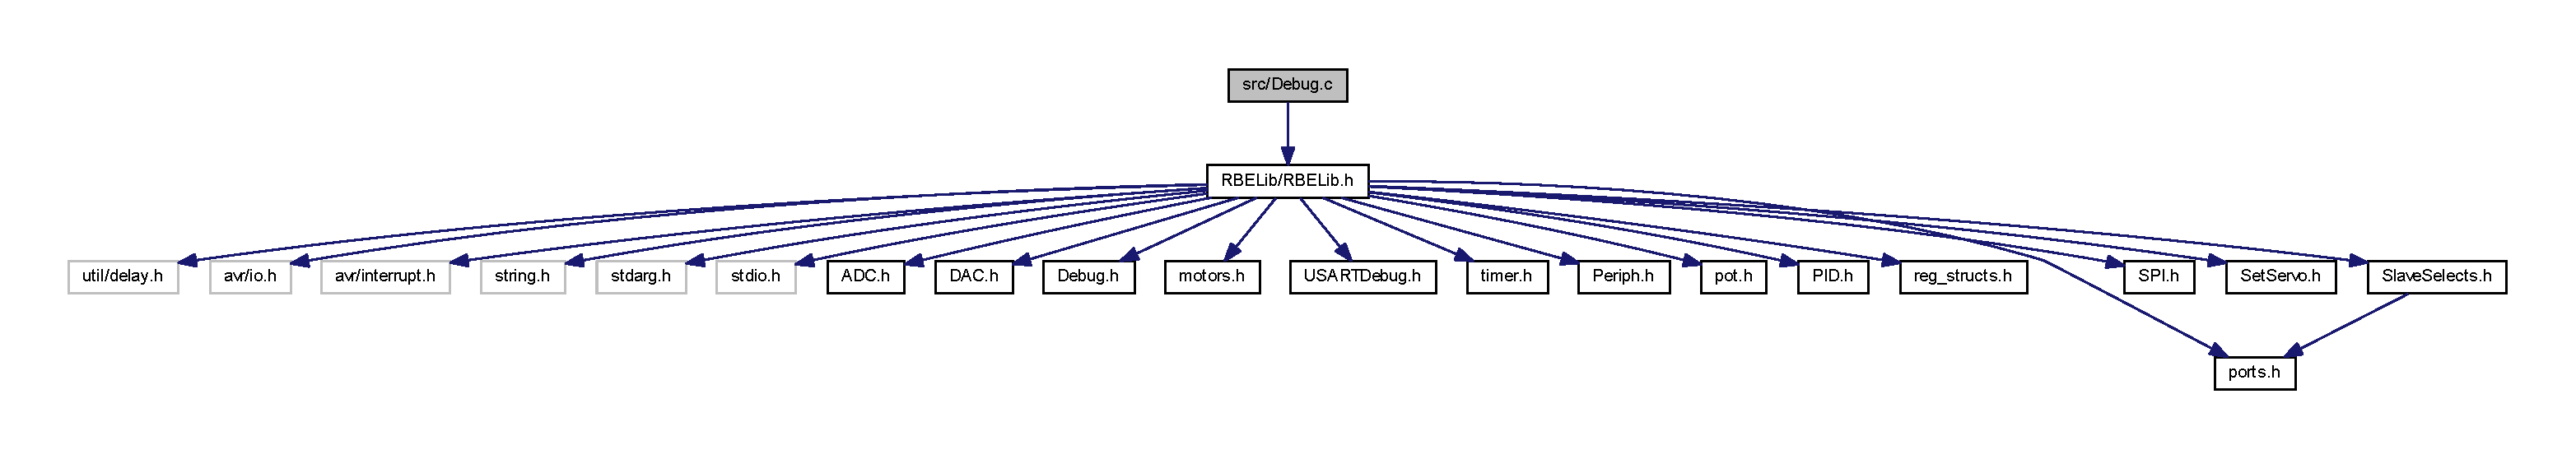
\includegraphics[width=350pt]{_debug_8c__incl}
\end{center}
\end{figure}
\subsection*{Functions}
\begin{DoxyCompactItemize}
\item 
int \hyperlink{_debug_8c_a450add2014d3b1c410c4225da137269a}{printf\-R\-B\-E} (char var, F\-I\-L\-E $\ast$stream)
\begin{DoxyCompactList}\small\item\em Calls the students function '\hyperlink{_u_s_a_r_t_debug_8h_ab52220b9802762326175f5a6d09c50a1}{put\-Char\-Debug()}' to output the stream to. You should not call this function directly, instead use the standard function printf(). \end{DoxyCompactList}\item 
void \hyperlink{_debug_8c_af447ccfe0edd5c2eee6ff9aba36bd6f9}{init\-R\-B\-E\-Lib} ()
\begin{DoxyCompactList}\small\item\em Rebinds stdout to call \hyperlink{_debug_8h_a450add2014d3b1c410c4225da137269a}{printf\-R\-B\-E()} and initializes communication with the coprocessor. This function should be called once at the start of your code once you have \hyperlink{_u_s_a_r_t_debug_8h_ab52220b9802762326175f5a6d09c50a1}{put\-Char\-Debug()} written in Lab 1. If you do not call this, printf() and Set\-Servo() will not work. \end{DoxyCompactList}\end{DoxyCompactItemize}


\subsection{Detailed Description}
Allows for printf() and \hyperlink{_set_servo_8h_aacba653c33e27af6b2ea227100a4217b}{set\-Servo()} capability. \begin{DoxyAuthor}{Author}
Eric Willcox 
\end{DoxyAuthor}
\begin{DoxyDate}{Date}
July 9, 2014 
\end{DoxyDate}


Definition in file \hyperlink{_debug_8c_source}{Debug.\-c}.



\subsection{Function Documentation}
\hypertarget{_debug_8c_af447ccfe0edd5c2eee6ff9aba36bd6f9}{\index{Debug.\-c@{Debug.\-c}!init\-R\-B\-E\-Lib@{init\-R\-B\-E\-Lib}}
\index{init\-R\-B\-E\-Lib@{init\-R\-B\-E\-Lib}!Debug.c@{Debug.\-c}}
\subsubsection[{init\-R\-B\-E\-Lib}]{\setlength{\rightskip}{0pt plus 5cm}void init\-R\-B\-E\-Lib (
\begin{DoxyParamCaption}
{}
\end{DoxyParamCaption}
)}}\label{_debug_8c_af447ccfe0edd5c2eee6ff9aba36bd6f9}


Rebinds stdout to call \hyperlink{_debug_8h_a450add2014d3b1c410c4225da137269a}{printf\-R\-B\-E()} and initializes communication with the coprocessor. This function should be called once at the start of your code once you have \hyperlink{_u_s_a_r_t_debug_8h_ab52220b9802762326175f5a6d09c50a1}{put\-Char\-Debug()} written in Lab 1. If you do not call this, printf() and Set\-Servo() will not work. 



Definition at line 20 of file Debug.\-c.



References init\-Alt\-Com().



Here is the call graph for this function\-:\nopagebreak
\begin{figure}[H]
\begin{center}
\leavevmode
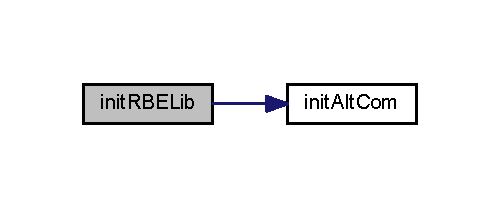
\includegraphics[width=240pt]{_debug_8c_af447ccfe0edd5c2eee6ff9aba36bd6f9_cgraph}
\end{center}
\end{figure}


\hypertarget{_debug_8c_a450add2014d3b1c410c4225da137269a}{\index{Debug.\-c@{Debug.\-c}!printf\-R\-B\-E@{printf\-R\-B\-E}}
\index{printf\-R\-B\-E@{printf\-R\-B\-E}!Debug.c@{Debug.\-c}}
\subsubsection[{printf\-R\-B\-E}]{\setlength{\rightskip}{0pt plus 5cm}int printf\-R\-B\-E (
\begin{DoxyParamCaption}
\item[{char}]{var, }
\item[{F\-I\-L\-E $\ast$}]{stream}
\end{DoxyParamCaption}
)}}\label{_debug_8c_a450add2014d3b1c410c4225da137269a}


Calls the students function '\hyperlink{_u_s_a_r_t_debug_8h_ab52220b9802762326175f5a6d09c50a1}{put\-Char\-Debug()}' to output the stream to. You should not call this function directly, instead use the standard function printf(). 


\begin{DoxyParams}{Parameters}
{\em var} & Character to output \\
\hline
{\em $\ast$stream} & Place to put the character (stdout) \\
\hline
\end{DoxyParams}


Definition at line 14 of file Debug.\-c.



References put\-Char\-Debug().



Here is the call graph for this function\-:\nopagebreak
\begin{figure}[H]
\begin{center}
\leavevmode
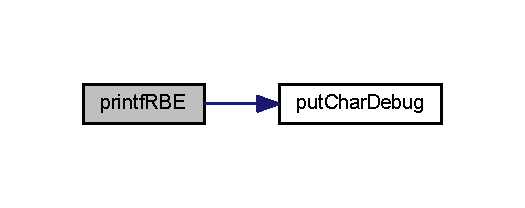
\includegraphics[width=252pt]{_debug_8c_a450add2014d3b1c410c4225da137269a_cgraph}
\end{center}
\end{figure}



%--- End generated contents ---

% Index
\newpage
\phantomsection
\addcontentsline{toc}{part}{Index}
\printindex

\end{document}
